\documentclass[11pt]{article}

% -------------------------------------------------
% Packages
% -------------------------------------------------
\usepackage[T1]{fontenc}
\usepackage[utf8]{inputenc}
\usepackage[english]{babel}
\usepackage[margin=.92in]{geometry}
\usepackage{microtype}
\usepackage[numbers]{natbib}
\usepackage[colorlinks=true,linkcolor=blue,citecolor=blue,urlcolor=blue]{hyperref}
\usepackage{url}

\usepackage{amsmath,amssymb,amsthm,mathtools,mathrsfs}
\usepackage{array,booktabs,tabularx,makecell}
\usepackage{graphicx,subcaption,float}
\usepackage{xcolor}
\usepackage{enumitem}
\usepackage{algorithm}
\usepackage{algpseudocode}
\usepackage[toc,page]{appendix}
\usepackage{cancel}

% -------------------------------------------------
% Theorem environments
% -------------------------------------------------
\theoremstyle{plain}
\newtheorem{thm}{Theorem}[section]
\newtheorem{cor}[thm]{Corollary}
\newtheorem{lem}[thm]{Lemma}
\newtheorem{prop}[thm]{Proposition}

\theoremstyle{definition}
\newtheorem{defn}[thm]{Definition}
\newtheorem{assumption}[thm]{Assumption}
\newtheorem{ex}[thm]{Example}

\theoremstyle{remark}
\newtheorem{rem}[thm]{Remark}

% -------------------------------------------------
% Commands
% -------------------------------------------------
\DeclarePairedDelimiter{\nint}{\lfloor}{\rceil}
\DeclarePairedDelimiter{\abs}{\lvert}{\rvert}

\newcommand{\R}{\mathbb{R}}
\newcommand{\EE}{\mathbb{E}}
\newcommand{\PP}{\mathbb{P}}
\newcommand{\op}{\mathrm{op}}
\newcommand{\tr}{\operatorname{tr}}
\newcommand{\rank}{\operatorname{rank}}
\newcommand{\card}{\operatorname{Card}}
\newcommand{\acc}{\operatorname{acc}}
\newcommand{\1}{\mathbf{1}}
\newcommand{\de}{\partial}
\newcommand{\eps}{\varepsilon}
\newcommand{\di}{\mathrm{d}}
\newcommand{\proofloc}[1]{\par\noindent\emph{Proof location.} #1\par}

\newcommand{\maybeincludegraphics}[2][]{%
  \IfFileExists{#2}{\includegraphics[#1]{#2}}{%
  \fbox{\parbox[c][2.2in][c]{0.92\linewidth}{\centering Missing figure: \detokenize{#2}}}}}

% -------------------------------------------------
% Title
% -------------------------------------------------
\title{\textbf{Pruning Deep Neural Networks via the Marchenko--Pastur Distribution}}

\author{
    Leonid Berlyand \\
    {\small Department of Mathematics} \\
    {\small Pennsylvania State University} \\
    {\small University Park, PA 16802, USA}
    \and
    Theo Bourdais\\
    {\small Department of Computing and Mathematical Sciences} \\
    {\small California Institute of Technology} \\
    {\small Pasadena, CA 91125, USA}
    \and
    Houman Owhadi\\
    {\small Department of Computing and Mathematical Sciences} \\
    {\small California Institute of Technology} \\
    {\small Pasadena, CA 91125, USA}
    \and
    Yitzchak Shmalo\thanks{Corresponding author: Yitzchak Shmalo. Email: \texttt{yitzchak.shmalo@gmail.com}.} \\
    {\small Department of Mathematics} \\
    {\small Pennsylvania State University} \\
    {\small University Park, PA 16802, USA}
}
\date{}

\begin{document}
\maketitle

\begin{abstract}
We propose a Random Matrix Theory (RMT)-based pruning method for pre-trained deep neural networks, with a focus on Vision Transformers (ViTs). The method uses Marchenko--Pastur diagnostics to estimate layerwise random-like bulk structure, and in the final ViT pipeline these diagnostics guide pruning and restoration budgets rather than hard singular-value truncation. Empirically, on ImageNet-trained ViT-B/16, the Hybrid Magnitude--SER protocol remains accurate through high unstructured sparsity: at \(70\%\) sparsity it retains \(78.01\%\) top-1 accuracy after a short frozen-mask fine-tuning pass, compared with \(67.44\%\) for the matched fine-tuned magnitude baseline and \(71.53\%\) for the classical RMT baseline.\footnote{The code used in this work can be found at \url{https://github.com/yspennstate/RMT_based_pruning_in_deep_learning}. The 17-model checkpoint archive for Table~\ref{tab:multi_arch_hybrid} is available at \url{https://drive.google.com/drive/folders/1mm990SHAHlYdISHxirvMRdVQEAjpIxDd}.}

On the theory side, we first prove a deterministic pruning certificate: any removed mask whose propagated data-path effect on the logits is small decreases an elastic-net regularized objective and preserves labels away from small margins. Gaussian and sub-Gaussian random-matrix assumptions then provide high-probability sufficient conditions for this certificate. We also analyze a stylized additive-noise model: persistent admissible randomness leaves an MP-type bulk, while under a one-sided stationarity hypothesis the bulk collapses, the surviving spike subspaces stabilize, and persistent positive spikes eventually become detectable outlier clusters. These results do not prove correctness of the full ViT pruning pipeline, but they clarify the role of random-like components and regularization in pruning.
\end{abstract}

\noindent\textbf{Keywords:} DNNs, ViTs, Random Matrix Theory, Marchenko--Pastur distribution, pruning, regularization

\noindent\textbf{Norm convention.}
Throughout, \(\|x\|_\infty\) denotes the vector maximum norm, while \(\|A\|_\infty\) denotes the induced matrix norm
\[
\|A\|_\infty:=\max_i\sum_j |A_{ij}|.
\]

\tableofcontents

% =================================================
\section{Introduction}
% =================================================

Deep neural networks (DNNs) have emerged as powerful tools in classification tasks, where elements of a set \(S \subset \R^n\) are categorized into one of finitely many classes.  They are a class of parametric functions, defined formally in Section~\ref{introduction_deep_neural_networks}.  Training a DNN on a labeled training set \(T \subset S\) consists of optimizing its parameters to minimize a loss--typically the cross-entropy loss of \eqref{CE}--so that the classification learned on \(T\) generalizes to the rest of \(S\).  DNNs have achieved remarkable empirical results across many domains, including handwriting recognition \cite{LBD}, image classification \cite{krizhevsky2017imagenet}, speech recognition \cite{hinton2012deep}, and natural language processing \cite{sutskever2014sequence}.  A central obstacle in DNN training is \emph{overfitting}: the model fits the training set so closely that it loses generalization to unseen data.  Standard countermeasures are dropout \cite{srivastava2014dropout}, early stopping \cite{prechelt2012early}, and weight-decay regularization \cite{Park2023}.

Random Matrix Theory (RMT) has recently emerged as a useful lens for understanding deep-learning spectra, overfitting, and implicit self-regularization \cite{martin2021implicit,mahoney2019traditional}.  This includes RMT-based stopping criteria \cite{meng2023impact}, regularization methods \cite{xiao2023heavy}, spectral analysis of weight matrices \cite{thamm2022random}, and studies of input--output Jacobians \cite{pastur2020random,pastur2023random}.  Investigations into RMT-based weight initializations have also been carried out \cite{saada2023initialisation}.  Several works further demonstrate that the spectral properties of trained weight matrices can predict generalization without access to a test set \cite{martin2021predicting,martin2020heavy}.  In this work, we extend that line of research by using spectral diagnostics not only to monitor a DNN, but to actively guide its pruning.  By identifying which weights have minimal impact on accuracy from a spectral perspective alone, we can compress a DNN while preserving its accuracy.

Pruning is one of the most classical tools for reducing DNN complexity, and a comprehensive review by Vadera et al.~\cite{vadera2022methods} groups pruning methods into three main strategies: magnitude-based pruning, redundancy identification through clustering, and sensitivity-analysis-based pruning.  Further surveys and channel-pruning methods are found in~\cite{cheng2023survey,khetan2020prunenet}.  Several previous studies have leveraged Singular Value Decomposition (SVD) to prune small singular values from DNN weight matrices, often using empirical heuristics like energy thresholds and validation-set error monitoring \cite{xue2013restructuring,cai2014fast,anhao2016svd,yang2020learning,xu2019trained}.  Our approach shares the broad goal of spectral compression but differs in two ways.  First, for ViTs we do \emph{not} use hard singular-value truncation in the final pipeline, because naively zeroing all bulk-scale singular values is empirically destructive: in modern trained transformers the bulk-scale subspace still encodes operationally important content.  Second, we use the Marchenko--Pastur (MP) law primarily as a \emph{diagnostic of randomness}, not as a claim that every trained layer is exactly ``MP plus a few spikes.''  The MP edge \(\sigma_+(\ell)\) becomes a layerwise allocation signal that decides \emph{where} to prune, while the prune--restore step decides \emph{how} to compensate for over-aggressive pruning.  For the classical case of fully-connected DNNs, our group has previously shown both numerically and theoretically that MP-based pruning can reduce a network's parameters by over \(99\%\) while increasing its accuracy~\cite{berlyand2023enhancing,shmalo2023deep}.

The goal of this paper is to develop pruning protocols for Vision Transformer (ViT) models that work directly from spectral diagnostics, with no access to a validation or test set during the pruning step.  Our head-to-head DeiT comparison in Section~\ref{subsec:deit_prior_comparison} is benchmarked against four representative DeiT pruning baselines: VTP \cite{zhu2021visual}, PoWER-BERT \cite{goyal2020powerbert}, HVT \cite{pan2021scalable}, and CP-ViT \cite{song2022cp}, the four head-to-head DeiT pruning methods reported by CP-ViT.  
Modern trained networks often show strong spectral heterogeneity.  Some layers are close to MP; others are non-MP or even heavy tailed \cite{martin2021implicit,mahoney2019traditional}.  This heavy-tailed regime is commonly interpreted as evidence of strong, scale-free correlations in the weights induced by optimization and implicit self-regularization, and it provides a more mechanistic explanation of generalization than viewing spectra through the narrow lens of ``MP plus a few spikes.''  Our approach uses spectral diagnostics to guide pruning, but relies on a complementary signal: rather than assume pervasive heavy tails, we measure how well each layer is described by MP.  Empirically, for ViTs we often observe layers whose spectra are not heavy-tailed and instead fit the MP distribution closely (Figure~\ref{fig:vit_mp_diagnostics}); for such layers our MP-fit and bulk metrics indicate that many parameters behave as random-like noise, and we prune them aggressively.  Layers that deviate from MP are treated more conservatively.  A natural extension is a hybrid scheme that applies a heavy-tail criterion to non-MP layers and the MP-fit criterion to those that match the MP distribution.

The empirical focus of this paper is on ViTs.  ViTs are central to modern image classification, most of their parameters sit in dense affine maps, and their layer spectra are particularly amenable to RMT diagnostics \cite{dosovitskiy2021image,vaswani2017attention}.  In principle the same MP diagnostics extend to other architectures--Convolutional Neural Networks, ResNets, and Swin/ConvNeXt-style hierarchical models--and the multi-architecture sweep of Section~\ref{subsec:architecture_validation} provides initial evidence that the Hybrid Magnitude--SER protocol transfers across these families with no per-architecture tuning.  We focus the main theoretical and pre-FT analysis on the plain ViT family in this paper because their layer spectra are particularly clean MP fits and their pruning literature is the densest.

On the theoretical side, the main general result is a deterministic certificate for actual pruning masks.  It says that if the removed mask has small propagated effect on the logits, then pruning decreases an elastic-net regularized objective and preserves labels with sufficient margin.  Gaussian and sub-Gaussian perturbation bounds supply high-probability sufficient conditions for this certificate.  We then analyze a stylized additive-noise model for one or several pruned layers: under a negligible structured--random cross term and one-sided directional stationarity, the admissible random part must be small whenever the regularized objective is nearly stationary in the pruning direction.  The Gaussian three-layer model in Appendix~\ref{Main_theory} is treated as a concrete spectral interpretation of this abstract framework.  The accompanying spectral consequence is that any admissible random component that remains at MP scale leaves a persistent MP-type bulk in the singular spectrum, while in the square Gaussian finite-rank deformation model there can be at most finitely many outliers.  These mathematical results do \emph{not} prove correctness of the full ViT pruning pipeline, but they clarify the role of random-like components and regularization in pruning.

The paper is organized as follows.  Section~\ref{sec:randomness} reviews DNN and MP preliminaries.  Section~\ref{sec:pruning_VITs} presents the ViT pruning procedure and the empirical results, including the head-to-head DeiT comparison with VTP/PoWER/HVT/CP-ViT and the multi-architecture validation across DeiT, Swin, ConvNeXt, ResNet, ViT, and Hiera checkpoints.  Section~\ref{sec:abstract_additive_extensions} gives the abstract additive perturbation framework, and Section~\ref{Main_theory_gen} contains the deterministic mask certificates, prune--restore certificate, stationarity consequences, and Gaussian/sub-Gaussian sufficient conditions for the data-path budget.  Appendix~\ref{Main_theory} records the stylized Gaussian specialization and spectral interpretation.  Supporting numerical material, proofs, and algorithms are deferred to the appendices.

% =================================================
\section{Randomness in Deep Neural Networks}
\label{sec:randomness}
% =================================================

\subsection{Introduction to Deep Neural Networks}
\label{introduction_deep_neural_networks}

In classification tasks, the goal is to assign each element of a set \(S\) to one of \(K\) classes. Let \(C(s)\in\{1,\dots,K\}\) denote the correct class of \(s\in S\). Given a labeled training set \(T\subset S\), we seek a classifier that generalizes from \(T\) to unseen data. We consider DNNs of the form
\[
\phi(\cdot,\alpha)=\rho\circ X(\cdot,\alpha),
\]
where \(\rho\) is the softmax map and \(X(\cdot,\alpha)\) is a composition of affine maps and nonlinearities:
\[
X(\cdot,\alpha)=\lambda\circ M_L(\cdot,\alpha)\circ\cdots\circ\lambda\circ M_1(\cdot,\alpha).
\]
Here:
\begin{itemize}[leftmargin=2em]
\item \(M_k(\cdot,\alpha)\) is an affine map \(\R^{N_{k-1}}\to\R^{N_k}\) with weight matrix \(W_k\in\R^{N_k\times N_{k-1}}\) and bias vector \(\beta_k\in\R^{N_k}\), so \(M_k(x)=W_kx+\beta_k\).
\item \(\lambda:\R^m\to\R^m\) is a nonlinear activation. In the simplified theory below we take \(\lambda\) to be either the coordinatewise absolute value or ReLU.
\item The softmax map \(\rho:\R^K\to\R^K\) is given by
\begin{equation}
\label{soft_max_new}
\rho(v)_i=\frac{e^{v_i}}{\sum_{j=1}^{K} e^{v_j}},\qquad v\in\R^K.
\end{equation}
\end{itemize}
The standard cross-entropy loss is
\begin{equation}
\label{CE}
L_{\mathrm{CE}}(\alpha)=-\frac{1}{|T|}\sum_{s\in T}\log\big(\phi_{C(s)}(s,\alpha)\big).
\end{equation}

Training a DNN means searching a high-dimensional, nonconvex loss landscape. Such landscapes typically contain local minima, saddle points, and flat regions \cite{dauphin2014identifying,choromanska2015loss}. In this context, RMT offers a useful language for distinguishing structured spectral behavior from random-like spectral bulk.

\subsection{The MP distribution in machine learning contexts}
\label{sec:MP_distribution}

The Marchenko--Pastur distribution is a basic object in RMT with applications in signal processing, statistics, wireless communication, and machine learning \cite{vershynin2018high,ge2021large,serdobolskii2000multivariate,couillet2011random}. We first define the relevant empirical spectral distributions.

\begin{defn}[Eigenvalue and singular-value empirical spectral distributions]
\label{ESD_Definition}
Let \(G\in\R^{N\times M}\), and let \(s_1(G),\dots,s_{\min\{N,M\}}(G)\) denote its singular values, counted with multiplicity and including possible zeros. The singular-value empirical spectral distribution (ESD) of \(G\) is
\[
\nu_G:=\frac{1}{\min\{N,M\}}\sum_{i=1}^{\min\{N,M\}}\delta_{s_i(G)}.
\]
If \(A\in\R^{M\times M}\) is symmetric positive semidefinite with eigenvalues \(\lambda_1(A),\dots,\lambda_M(A)\), its eigenvalue ESD is
\[
\mu_A:=\frac{1}{M}\sum_{i=1}^M \delta_{\lambda_i(A)}.
\]
\end{defn}

\begin{thm}[Marchenko--Pastur law]
\label{RMT_MP_theorem}
Let \(W_N\) be an \(N\times M_N\) random matrix with i.i.d.\ entries of mean \(0\), variance \(\sigma^2\), and finite fourth moment. Define
\[
X_N:=\frac{1}{N}W_N^\top W_N,
\qquad c_N:=\frac{M_N}{N}\to c\in(0,\infty).
\]
Then the eigenvalue ESD \(\mu_{X_N}\) converges almost surely to the Marchenko--Pastur law
\begin{equation}
\label{MP_distribution}
\mu_{\mathrm{MP}}^{c,\sigma^2}
=
\left(1-\frac{1}{c}\right)_+\delta_0
+
\frac{\sqrt{(\lambda_+-x)(x-\lambda_-)}}{2\pi c\sigma^2 x}\,
\1_{[\lambda_-,\lambda_+]}(x)\,\di x,
\end{equation}
where
\begin{equation}
\label{lambda_parameters}
\lambda_\pm=\sigma^2(1\pm \sqrt c)^2.
\end{equation}
\end{thm}
\proofloc{This is a classical cited random-matrix input rather than a new theorem of the paper; see Appendix~\ref{app:external_rmt_inputs} for source notes.}

\begin{rem}
If \(M_N\le N\) for all \(N\), then \(c\in(0,1]\) and the atom at zero in \eqref{MP_distribution} vanishes. When discussing the singular-value scale of \(W_N\), we write
\[
\sigma_+ := \sqrt{N\lambda_+}
\]
for the corresponding MP upper edge.
\end{rem}

\subsection{Reduction of randomness in DNN weights via MP diagnostics}
\label{overallpicture}

At initialization, many DNN weight matrices are approximately i.i.d.\ with variance of order \(1/N\). In that regime, the singular values are \(O(1)\). More precisely, if \(W_{ij}\) has variance \(g/N\), then the nonzero eigenvalues of \(W^\top W\) are on the \(O(1)\) scale, whereas the eigenvalues of
\[
X_\ell=\frac{1}{N}W_\ell^\top W_\ell
\]
are on the \(O(1/N)\) scale and follow the MP law with variance parameter \(g/N\). Equivalently, if \(\lambda_+\) is the fitted right edge for \(X_\ell\), then the corresponding singular-value edge of \(W_\ell\) is
\[
\sigma_+=\sqrt{N\lambda_+}=\sqrt g\,(1+\sqrt c)
\]
in the rectangular aspect-ratio limit \(M/N\to c\). During training, learned structure appears and the spectra deviate from the initial random law \cite{martin2021implicit,staats2022boundary}. This motivates the heuristic decomposition
\[
W_\ell(t)=R_\ell(t)+S_\ell(t),
\]
where \(R_\ell(t)\) is a random-like part and \(S_\ell(t)\) is a structured part learned from the data.

\paragraph{Supposition 1.}
After \(t\) training steps, the layer-\(\ell\) weight matrix can be decomposed as
\[
W_\ell(t)=R_\ell(t)+S_\ell(t),
\]
where \(R_\ell(t)\) is an independent random perturbation and \(S_\ell(t)\) is a structured signal component.

\paragraph{Supposition 2.}
For the spectral spike interpretation, \(S_\ell(t)\) is low rank or approximately low rank relative to the width.

These suppositions are not meant as exact descriptions of trained ViTs. Rather, they motivate a spectral diagnostic: layers that look more MP-like are treated as more random-like, while layers that deviate strongly from MP are pruned more conservatively.

\noindent\textbf{Spectral heterogeneity and quasi-rank reduction.}
Modern trained transformers exhibit substantial layer-wise spectral heterogeneity: some weight matrices are well described by an MP bulk, whereas others deviate markedly and can even be heavy tailed \cite{martin2021implicit,mahoney2019traditional}. Consequently, in our numerical pipeline we do not assume a clean global ``MP plus spikes'' model. Instead, we use MP only as a \emph{diagnostic}. For each layer we estimate the fitted MP edge \(\sigma_+\) via a BEMA-style fit \cite{ke2021estimation}, store auxiliary statistics such as MP-fit error and the Hill exponent, and use these quantities to allocate layerwise pruning and restoration budgets. Singular-vector sparsification experiments are retained in the appendix as diagnostics; the final pruning protocols operate on unstructured weight masks and use the MP fit to decide \emph{where} magnitude pruning and restoration should occur.

\noindent\textbf{Theoretical assumptions: no ``small = noise'' requirement.}
Our theory likewise does not assume that all small singular values are noise or that informative directions cannot lie inside the bulk. The loss theorems require only a negligible structured-random cross term (verified in the Gaussian specialization by \(\|S\|_F=o(\sqrt N)\)); finite-rank or approximate-low-rank assumptions are used only for the spectral corollaries. The random component \(R\) is assumed independent with variance scaling \(O(1/N)\). In particular, we do not require spectral separation at the MP edge.

% =================================================
\section{Numerical evidence: RMT-guided pruning of ViTs}
\label{sec:pruning_VITs}
% =================================================

Vision Transformers are a natural testbed for the Marchenko--Pastur diagnostics developed above: most of the parameters in a ViT lie in dense attention and MLP projection matrices \cite{dosovitskiy2021image,vaswani2017attention}.  The numerical evidence motivates separating the methods into four increasingly practical protocols.  Compact definitions are given here; the full operational descriptions, all hyperparameters, and the sweeps used to select them are in Appendix~\ref{app:splus_budget}.
\begin{enumerate}[leftmargin=2em]
\item \textbf{Global magnitude pruning} (\emph{Classical magnitude}), the standard unstructured baseline: at sparsity \(s\), the \(s\)-fraction of weights with smallest absolute value across the prunable layers is set to zero, followed by one matched fine-tuning epoch.  Used as the reference column ``Classical magnitude'' in Tables~\ref{tab:vitb_current_methods} and~\ref{tab:multi_arch_hybrid}; full schedule in Appendix~\ref{subsec:splus_method}.
\item \textbf{Classical RMT pruning} (\emph{Classical RMT}), the cycle-based RMT method retained as a diagnostic baseline: fit a per-layer Marchenko--Pastur edge \(\sigma_+(\ell)\), treat sub-edge singular components as bulk-like, sparsify small singular-vector coordinates, and prune the resulting coefficients directly.  Defined in detail in Appendix~\ref{subsec:classical_rmt}.
\item \textbf{Spectral Edge Budgeting} (SEB), a no-fine-tuning method that uses the fitted MP upper edge \(\sigma_+(\ell)\), together with the Hill exponent \(\alpha_\ell\) at very low sparsity, to allocate a layerwise magnitude-pruning budget.  Hyperparameters \((\beta,s_{\mathrm{d}},p)\), the layer-type extension, and the sparsity-regime selection rule are defined in Appendix~\ref{subsec:splus_method}; the SEB-vs-magnitude comparison is Table~\ref{tab:final_comparison} (mask-only) and Table~\ref{tab:final_comparison_10k} (full validation).
\item \textbf{Spectral Edge Reallocation} (SER), the main RMT prune--restore method: prune beyond the target, form a reservoir of removed weights, reinsert an RMT-ranked budget, and run a short frozen-mask fine-tuning phase.  Defined in Appendix~\ref{subsec:ser_method}.  The \emph{Hybrid Magnitude--SER} protocol used in Tables~\ref{tab:vitb_current_methods} and~\ref{tab:multi_arch_hybrid} uses exact global magnitude pruning up to \(s=0.20\) and then switches to SER for \(s\ge0.25\); see Appendix~\ref{subsec:hybrid_ser_method}.
\end{enumerate}

\subsection{Protocols and RMT parameter selection}
\label{pruning_strategy}

All reported ViT-B/16 numbers use the same ImageNet-1k validation set \cite{5206848} and the same checkpoint, \path{vit_base_patch16_224.augreg2_in21k_ft_in1k}, unless explicitly stated otherwise.  For each target layer \(W_\ell\), we fit the MP bulk of \(W_\ell^\top W_\ell/N\) using the BEMA procedure of Appendix~\ref{numerics_updated}.  The resulting layer bank stores \(\sigma_+(\ell)\), MP-fit error, bulk fraction, and the Hill exponent \(\alpha_\ell\).  The pruning rules do not refit these quantities during a run.

The SEB parameters were selected by the sweep in Appendix~\ref{app:splus_budget}: first a signal comparison, then decay-shape and layer-type sweeps, and finally full-validation evaluation of the selected configuration.  The main empirical lesson of that appendix is that the MP edge is weak at very low sparsity but becomes highly informative once magnitude pruning approaches the accuracy cliff.  Consequently, the hybrid protocol intentionally uses exact magnitude pruning through \(20\%\) sparsity and activates RMT-guided reallocation only after the regime where magnitude is already near-optimal.

\subsection{ViT-B/16 results}
\label{subsec:vitb_current_results}

Table~\ref{tab:vitb_current_methods} summarizes the fine-tuned ViT-B/16 evidence.  The no-fine-tuning mask-only comparison is separated into Appendix~\ref{subsec:final_comparison_10k}; the main table compares methods under matched post-pruning validation with a short frozen-mask fine-tuning pass where applicable.

\begin{table}[ht]
\centering
\caption{Fine-tuned ViT-B/16 pruning comparison on ImageNet-1k validation.  Entries are top-1 accuracy (\%) at sparsity \(s\) (fraction of weights set to zero in the prunable layers).  Classical magnitude (Appendix~\ref{subsec:splus_method}) and Classical RMT (Appendix~\ref{subsec:classical_rmt}) use the matched one-cycle fine-tuning protocol.  SER (Appendix~\ref{subsec:ser_method}) uses the prune--restore procedure with a short frozen-mask fine-tuning phase.  Hybrid Magnitude--SER (Appendix~\ref{subsec:hybrid_ser_method}) uses exact global magnitude pruning through \(s=0.20\) and then SER for \(s\ge0.25\).  A dash means that the archived run contains no completed full-validation checkpoint at that sparsity.  Dense baseline: \(85.11\%\).}
\label{tab:vitb_current_methods}
\scriptsize
\setlength{\tabcolsep}{2.5pt}
\begin{tabular}{lcccccccccccccc}
\toprule
Method & \(0.05\) & \(0.10\) & \(0.15\) & \(0.20\) & \(0.25\) & \(0.30\) & \(0.35\) & \(0.40\) & \(0.45\) & \(0.50\) & \(0.55\) & \(0.60\) & \(0.65\) & \(0.70\) \\
\midrule
Classical magnitude   & 85.21 & 85.16 & 85.08 & 84.87 & 84.65 & 84.46 & 84.08 & 83.53 & 82.86 & 81.67 & 80.17 & 77.98 & 74.30 & 67.44 \\
Classical RMT         & 85.21 & 85.14 & 85.01 & 84.97 & 84.77 & 84.55 & 84.31 & 83.98 & 83.31 & 82.57 & 81.31 & 79.13 & 76.46 & 71.53 \\
SER                   & 84.94 & 84.98 & 84.82 & 84.76 & 84.66 & 84.55 & 84.41 & 84.24 & 83.73 & 83.27 & 82.65 & 81.33 & 79.95 & 77.94 \\
Hybrid Magnitude--SER & 85.23 & 85.17 & 85.06 & 84.89 & 84.81 & 84.64 & 84.55 & 84.28 & 83.80 & 83.37 & 82.76 & 81.39 & 79.95 & 78.01 \\
\bottomrule
\end{tabular}
\end{table}

The matched fine-tuned comparison shows a widening RMT advantage as sparsity increases.  Classical RMT improves over the classical magnitude baseline by \(1.15\) pp at \(s=0.60\), \(2.16\) pp at \(s=0.65\), and \(4.09\) pp at \(s=0.70\).  The direct SER sweep is competitive through moderate sparsity but becomes unstable by \(s=0.65\).  The hybrid protocol is stronger in that regime: at \(s=0.70\), Hybrid Magnitude--SER reaches \(78.01\%\) top-1, improving over classical RMT by \(6.48\) pp and over classical magnitude by \(10.57\) pp.

The hybrid run is motivated by the low-sparsity sweep in Appendix~\ref{app:splus_budget}: at \(s\le0.20\), RMT modulation is unnecessary and sometimes slightly worse than exact magnitude pruning; beyond that point, the spectral budget becomes useful.  The completed hybrid entries retain essentially dense accuracy through \(35\%\) sparsity and remain above both classical baselines through \(70\%\).

\subsection{Interpretation}
\label{subsec:current_numerics_interpretation}

These results change the numerical story in two ways.  First, the classical RMT procedure is not the final ViT method.  It verifies that MP-bulk structure is visible in trained layers, but directly operating on sub-edge singular components is too brittle for modern ViTs.  Second, the effective use of RMT is \emph{budget allocation}: MP-like layers and MLP projections can absorb more pruning, while attention projections often need more protection.  This matches the deterministic theory in Section~\ref{Main_theory_gen}: once a mask is fixed, the relevant object is the perturbation induced on the network's data path, and the MP edge acts as a layerwise proxy for where that perturbation is more likely to be admissible.

\subsection{Broader architecture validation}
\label{subsec:architecture_validation}

To test transfer beyond a single ViT checkpoint, we apply the same hybrid protocol to a deliberately diverse architecture set: AugReg ViT-B/ViT-S/ViT-L checkpoints \cite{dosovitskiy2021image,steiner2022how}, DeiT \cite{touvron2021training}, Swin \cite{liu2021swin}, ConvNeXt \cite{liu2022convnet}, ResNet \cite{he2016deep}, and Hiera \cite{ryali2023hiera}.  These models cover plain token mixers, windowed transformers, hierarchical transformers, and ConvNet architectures designed to match transformer-scale performance.  Dense checkpoint baselines are taken from the corresponding pretrained model records in \texttt{timm} \cite{rw2019timm}, using the ImageNet-1k validation top-1 reported for each checkpoint when available.  Additional candidates such as SwinV2 \cite{liu2022swinv2}, BEiT \cite{bao2022beit}, EVA-02 \cite{fang2023eva02}, MaxViT \cite{tu2022maxvit}, CoAtNet \cite{dai2021coatnet}, MViTv2 \cite{li2022mvitv2}, DaViT \cite{ding2022davit}, PVTv2 \cite{wang2022pvtv2}, XCiT \cite{elnouby2021xcit}, CaiT \cite{touvron2021going}, VOLO \cite{yuan2021volo}, and CrossViT \cite{chen2021crossvit} are natural extensions, but they are not included in the validated table unless a full ImageNet-1k checkpoint validation was produced.

The architectural rows should be compared against the corresponding dense model papers and checkpoint records.  Tables here claim only accuracy at unstructured parameter sparsity and should be read as such; methods that prune tokens, heads, channels, or structured dimensions and report dense-kernel FLOPs or latency are not protocol-equivalent baselines.

Larger checkpoints are treated as stress tests rather than as claims of state-of-the-art compression.  On an A40, the practical constraint is memory, so larger models require smaller batches and longer wall-clock time while preserving the same mask construction, RMT cache, and post-pruning validation protocol.  Table~\ref{tab:multi_arch_hybrid} reports larger-model checkpoints that produced at least one completed full-validation result.

Table~\ref{tab:multi_arch_hybrid} reports the multi-architecture validation ledger in one place.  Unmarked rows use the canonical Hybrid Magnitude--SER protocol (Appendix~\ref{subsec:hybrid_ser_method}: exact magnitude pruning through \(s=0.20\), SER thereafter); rows marked \(\ddagger\) use the adaptive variant that terminates stage-1 once the post-FT top-1 drops by more than \(0.7\) percentage points relative to the dense baseline.  The displayed table contains 17 model rows after omitting the two partial ViT-Small/16 and Swin-Small ledgers.  The ViT-B/16 row reproduces the Table~\ref{tab:vitb_current_methods} canonical row for cross-reference.  ResNet101d uses the timm reference baseline at its native train resolution (256$\times$256, baseline top-1 \(82.26\%\)).

The pattern at the low-sparsity end of Table~\ref{tab:multi_arch_hybrid} is consistent across architectures: through \(s=0.20\), the exact-magnitude prefix (Appendix~\ref{subsec:splus_method}) recovers (and at \(s\le 0.10\) often slightly exceeds) the dense baseline after a single fine-tuning epoch on every architecture for which a datapoint is available.  The decisive sparsities for the hybrid protocol lie at \(s\ge 0.45\), where Table~\ref{tab:vitb_current_methods} establishes that classical magnitude (Appendix~\ref{subsec:splus_method}) and classical RMT (Appendix~\ref{subsec:classical_rmt}) cannot match the SER-based methods.  Appendix~\ref{subsec:checkpoint_validation_ledger} gives the checkpoint-level validation ledger used to populate these tables, and Table~\ref{tab:additional_downloaded_validation_ledger} records the downloaded threshold and restart ledgers retained for auditability.

\begin{table}[ht]
\centering
\caption{\textbf{Multi-architecture Hybrid Magnitude--SER sweep on ImageNet-1k validation.}  Entries are post-fine-tuning top-1 accuracy (\%) at sparsity \(s\).  The table contains 17 model rows after omitting the two partial ViT-Small/16 and Swin-Small ledgers.  Unmarked rows use the canonical protocol of Appendix~\ref{subsec:hybrid_ser_method}: exact global magnitude pruning (Appendix~\ref{subsec:splus_method}) through \(s=0.20\) followed by SER (Appendix~\ref{subsec:ser_method}) for \(s\ge0.25\).  Rows marked \(\ddagger\) use the adaptive drop-threshold variant: stage-1 terminates once the post-FT top-1 drops by more than \(0.7\) percentage points relative to the dense baseline, and SER resumes from the next sparsity step.  ``Baseline'' is the dense top-1 of each pretrained checkpoint as reported by \texttt{timm} \cite{rw2019timm} and the corresponding model/checkpoint sources on ImageNet-1k validation.  The ViT-B/16 row matches the corresponding row of Table~\ref{tab:vitb_current_methods}.}
\label{tab:multi_arch_hybrid}
\tiny
\setlength{\tabcolsep}{1.0pt}
\begin{tabular}{lccccccccccccccc}
\toprule
Architecture (timm checkpoint) & Base. & \(0.05\) & \(0.10\) & \(0.15\) & \(0.20\) & \(0.25\) & \(0.30\) & \(0.35\) & \(0.40\) & \(0.45\) & \(0.50\) & \(0.55\) & \(0.60\) & \(0.65\) & \(0.70\) \\
\midrule
ViT-B/16 \texttt{augreg2\_in21k\_ft\_in1k} & 85.11 & 85.23 & 85.17 & 85.06 & 84.89 & 84.81 & 84.64 & 84.55 & 84.28 & 83.80 & 83.37 & 82.76 & 81.39 & 79.95 & 78.01 \\
ViT-B/16/384 \texttt{augreg\_in21k\_ft}    & 86.01 & 86.05 & 86.09 & 86.07 & 85.99 & 86.00 & 85.90 & 85.81 & 85.78 & 85.48 & 85.15 & 84.64 & 83.35 & 82.50 & 81.33 \\
ViT-Large/16 \texttt{augreg\_in21k\_ft}    & 85.84 & 85.80 & 85.84 & 85.88 & 85.75 & 84.98 & 85.32 & 85.64 & 85.04 & 85.08 & 84.52 & 84.34 & 83.81 & 83.02 & 82.13 \\
DeiT-Tiny \texttt{patch16\_224.fb\_in1k}   & 72.21 & 72.41 & 72.38 & 72.18 & 71.86 & 71.99 & 71.75 & 71.35 & 70.66 & 68.97 & 67.74 & 65.91 & 61.17 & 55.58 & 52.55 \\
DeiT-Small \texttt{patch16\_224.fb\_in1k}  & 79.85 & 79.82 & 79.78 & 79.62 & 79.37 & 79.31 & 79.21 & 79.00 & 78.61 & 78.06 & 77.22 & 76.25 & 74.14 & 72.05 & 68.55 \\
DeiT-Base \texttt{patch16\_224.fb\_in1k}   & 81.80 & 81.76 & 81.70 & 81.58 & 81.46 & 81.42 & 81.28 & 81.17 & 80.99 & 80.62 & 80.12 & 79.49 & 78.16 & 76.72 & 74.90 \\
Swin-Tiny \texttt{patch4\_window7\_224}    & 81.20 & 81.32 & 81.28 & 81.25 & 81.05 & 81.09 & 80.91 & 80.78 & 80.37 & 80.14 & 79.80 & 78.98 & 78.06 & 76.64 & 74.47 \\
ConvNeXt-Base \texttt{in22k\_ft\_in1k}     & 85.84 & 85.72 & 85.58 & 85.51 & 85.26 & 85.35 & 85.39 & 85.26 & 85.04 & 84.94 & 84.80 & 84.09 & 83.70 & 83.11 & 81.21 \\
ResNet50d \texttt{ra2\_in1k}               & 80.55 & 79.90 & 80.01 & 80.02 & 80.12 & 80.09 & 80.12 & 80.06 & 79.90 & 79.48 & 79.16 & 78.93 & 77.93 & 77.25 & 76.32 \\
ResNet101d \texttt{ra2\_in1k}              & 82.26 & 82.06 & 82.05 & 82.15 & 82.15 & 82.06 & 82.07 & 81.93 & 81.97 & 81.61 & 81.56 & 81.47 & 80.45 & 80.15 & 79.82 \\
Hiera-Base+ \texttt{mae\_in1k\_ft\_in1k}   & 84.40 & 85.04 & 84.94 & 84.76 & 84.39 & 77.95\protect\footnotemark & 83.12 & 82.15 & 82.37 & 82.29 & 82.25 & 82.00 & 80.03 & 80.55 & 78.96 \\
ResNet18 \texttt{tv\_in1k}$^{\ddagger}$    & 69.76 & 69.73 & 69.52 & 69.18 & 68.94 & 69.02 & 69.28 & 69.50 & 69.50 & 69.39 & 69.12 & 69.00 & 68.31 & 67.82 & 67.23 \\
ResNet34 \texttt{tv\_in1k}$^{\ddagger}$    & 73.28 & 73.00 & 72.67 & 72.39 & 72.62 & 73.06 & 73.09 & 73.16 & 73.16 & 73.00 & 72.88 & 72.74 & 72.12 & 71.59 & 71.44 \\
ResNet50 \texttt{tv\_in1k}$^{\ddagger}$    & 76.13 & 75.85 & 75.33 & 75.72 & 76.07 & 76.17 & 76.13 & 76.13 & 76.14 & 75.75 & 75.76 & 75.70 & 74.83 & 74.62 & 74.15 \\
DeiT-Base \texttt{patch16\_224.fb\_in1k}$^{\ddagger}$ & 81.97 & 81.79 & 81.69 & 81.54 & 81.44 & 81.25 & 81.35 & 81.18 & 80.95 & 80.68 & 80.12 & 79.48 & 78.24 & 76.70 & 74.78 \\
Swin-Tiny \texttt{patch4\_window7\_224}$^{\ddagger}$ & 81.39 & 81.32 & 81.29 & 81.26 & 81.05 & 80.77 & 80.47 & 80.58 & 80.43 & 80.11 & 79.80 & 78.94 & 78.03 & 76.53 & 74.31 \\
ConvNeXtV2-Base \texttt{fcmae\_ft\_in22k\_in1k}$^{\ddagger}$ & 86.72 & 86.67 & 86.58 & 86.43 & 86.27 & 85.93 & 85.97 & 85.96 & 85.71 & 85.58 & 85.33 & 84.81 & 84.61 & 83.83 & 81.40 \\
\bottomrule
\end{tabular}
\end{table}
\footnotetext{The Hiera-Base+ entry at \(s=0.25\) reflects an unstable first stage-2 cycle in which the post-FT train-subset probe \emph{decreased} from \(96.09\%\) (post-prune) to \(90.63\%\) (post-FT), an abnormal regression of \(5.5\)~pp that propagated to a depressed val top-1.  The next stage-2 cycles recovered to \(83.12\%\) at \(s=0.30\), \(82.15\%\) at \(s=0.35\), \(82.37\%\) at \(s=0.40\), \(82.29\%\) at \(s=0.45\), \(82.25\%\) at \(s=0.50\), \(82.00\%\) at \(s=0.55\), \(80.03\%\) at \(s=0.60\), \(80.55\%\) at \(s=0.65\), and \(78.96\%\) at \(s=0.70\) with normal training dynamics, suggesting the cliff at \(s=0.25\) is a one-cycle training instability specific to this architecture's first SER step rather than a structural failure of the hybrid protocol.  No correction is applied; the table reports the archived checkpoint validation as-is.}

\begin{figure}[ht]
\centering

\includegraphics[width=\textwidth]{figures_param_vs_drop.pdf}
\caption{Top-1 accuracy drop after Hybrid Magnitude--SER pruning, plotted against dense parameter count on a log scale, for the 17 model rows retained in Table~\ref{tab:multi_arch_hybrid} after removing the two partial ViT-Small/16 and Swin-Small rows.  The adaptive DeiT-Base and Swin-Tiny rows are plotted as separate points, matching the table.  Each row is one point; no within-family averaging.  All three panels contain 17 points.  Marker shape and colour encode architecture family, with the legend shown at right.  Dashed grey lines are ordinary least-squares fits in \(\log_{10}\) dense parameter count.  The fitted slopes are \(-0.73\), \(-2.40\), and \(-4.18\) pp per decade of parameters at \(s=0.50\), \(s=0.60\), and \(s=0.70\), with \(R=-0.31\), \(R=-0.43\), and \(R=-0.41\), respectively.  The directional sign remains negative and the magnitude steepens with sparsity: smaller checkpoints lose more top-1 under the same protocol, with DeiT-Tiny losing \(19.66\) pp at \(s=0.70\) while the base/large checkpoints lose about \(3.7\)--\(7.2\) pp.}
\label{fig:param_vs_drop}
\end{figure}

\paragraph{Why the slope steepens with sparsity: a suggestive RMT-consistent pattern.}
Figure~\ref{fig:param_vs_drop} is consistent with the random-matrix view of pruning that this paper builds on, but we treat it as suggestive rather than confirmatory evidence.  At \(s=0.50\) the fitted slope in \(\log_{10}\) parameter count is already negative (\(-0.73\) pp per decade, \(R=-0.31\)); by \(s=0.70\) it has steepened to \(-4.18\) pp per decade (\(R=-0.41\)).  We caution that the full 17-row plot has modest cross-architecture correlations.  ``Larger models lose less under the same protocol'' is a coarse pattern compatible with several non-RMT explanations: overparameterization, training-recipe differences, architecture-family effects, baseline accuracy heterogeneity, layer width, or general parameter-distribution effects.  We make below the weaker claim that the \emph{systematic ordering} --- slope monotonically more negative as sparsity grows --- is a pattern that the random-matrix view of SER would predict, namely that each weight matrix decomposes (approximately) into a deterministic spike component carrying task signal and a Marchenko--Pastur-like bulk carrying random-matrix noise.

If that decomposition holds, the bulk fraction of any one matrix is roughly invariant across architectures of the same family, but the \emph{absolute} number of bulk components scales with the smaller matrix dimension, which in turn scales with model width and therefore with parameter count.  A \(\sim 6\) M-parameter model and a \(\sim 90\) M-parameter model can both afford to drop the same fraction of bulk components without crossing the spike-detection threshold; but at high target sparsity (\(s=0.70\)) the protocol is forced into the spike subspace of the small model long before it exhausts the bulk of the large model.  The fitted log-parameter slope steepening from \(-0.73\) to \(-4.18\) pp per decade between \(s=0.50\) and \(s=0.70\) quantifies this effect: the larger the architecture, the further the protocol can push into sparsity before the bulk reservoir runs out and signal-carrying spikes start to be removed.

This empirical pattern is suggestive of, though not confirmatory for, the RMT picture.  The predicted directional sign --- bigger model, smaller drop --- is observed in every panel; the magnitude of the slope grows roughly in lockstep with sparsity.  Most checkpoints remain close to the dense baseline at moderate sparsity, and the large departures appear once the protocol begins to remove components close to or beyond the MP edge --- the regime where classical RMT prediction starts to bite.  We do not interpret Figure~\ref{fig:param_vs_drop} as direct confirmation of the bulk-vs-spike decomposition; that would require per-layer measurements of the certificate quantities, which we report in Section~\ref{subsec:theory_numerics_alignment} below.  We do interpret it as evidence consistent with the central premise of the paper: as networks grow, the bulk-vs-spike decomposition that motivates SER appears to become a better description of where the prunable capacity lives, so the same protocol becomes more accuracy-preserving at scale.

\subsection{Connecting the deterministic certificates to the multi-architecture numerics}
\label{subsec:theory_numerics_alignment}

The deterministic mask certificate (Theorem~\ref{thm:deterministic_mask_certificate}) certifies that pruning a removed component \(R\) from a layer \(A=S+R\) decreases the elastic-net objective whenever the data-path budget satisfies
\begin{equation}
\label{eq:certificate_inequality_main}
B_T(R)\;<\;\lambda_2\|R\|_F^2+\lambda_1\|R\|_1,
\end{equation}
where \(B_T(R)\) is the data-path budget of Eq.~\eqref{eq:data_path_budget}.  In the iid-Gaussian sufficient-condition setting of Corollary~\ref{cor:mp_edge_data_path_budget}, the fitted MP singular-value edge \(\sigma_+(\ell)\) bounds the data-path budget up to a logarithmic factor and the data-dependent factors \(L_s\|v_s\|_2\); the actual magnitude-selected mask is deterministic and not iid Gaussian, so we use \(\sigma_+(\ell)\) as a heuristic per-layer ranking signal rather than as a certified bound on the realized \(B_T(R)\).  The prune--restore extension (Theorem~\ref{thm:deterministic_prune_restore_certificate}) refines~\eqref{eq:certificate_inequality_main} by splitting the removed mass into a kept reservoir \(Q\) and a finally-removed component \(P\), so that restoring \(Q\) strictly improves the certificate margin by \(B_T(P)-(\lambda_2\|P\|_F^2+\lambda_1\|P\|_1)\).  The remainder of this subsection compares the certificate-side prediction against the multi-architecture numbers in Table~\ref{tab:multi_arch_hybrid} and Figure~\ref{fig:param_vs_drop}.

\paragraph{Low sparsity \(s\le 0.20\).}  Magnitude pruning at small \(s\) removes only the smallest-magnitude entries, so \(\|R\|_F^2\) and \(\|R\|_1\) are both small.  Empirically, every architecture in Table~\ref{tab:multi_arch_hybrid} stays within \(\pm 0.5\) percentage points of its dense baseline through \(s=0.20\); the exact-magnitude prefix often \emph{slightly exceeds} the dense baseline at \(s\le 0.10\) after a single fine-tuning epoch.  This regime is consistent with the qualitative picture from Theorem~\ref{thm:deterministic_mask_certificate} and Lemma~\ref{lem:deterministic_ce_path_bound} (small removed mass should give a small data-path budget, hence a small CE perturbation), though we do not compute the literal certificate inequality~\eqref{eq:certificate_inequality_main} with the actual \(\lambda_1,\lambda_2\) used by Hybrid Magnitude--SER and therefore do not claim that the inequality is verified.

\paragraph{Moderate sparsity \(s\in[0.30,0.50]\).}  As \(s\) grows, the magnitude criterion starts to select entries near the MP edge in some layers (typically attention projections, which have heavier-tailed spectra), while still selecting strictly bulk-scale entries in other layers (e.g.\ MLP projections).  In the certificate language of Theorem~\ref{thm:deterministic_mask_certificate}, the per-layer ratio \(B_T(R_\ell)/(\lambda_2\|R_\ell\|_F^2+\lambda_1\|R_\ell\|_1)\) is expected to cross unity in some layers but not others.  Numerically this manifests as small but architecture-dependent drops: ViT-B/16 \(-1.74\), DeiT-Base \(-1.68\), ConvNeXt-Base \(-1.04\), ResNet50d \(-1.39\), ResNet101d \(-0.70\) (all at \(s=0.50\) relative to baseline).  We do not compute the literal multi-layer perturbation bound of Theorem~\ref{thm:deterministic_multilayer_mask_certificate}, so we do not claim the observed drops are within it; we report the cross-architecture variation as consistent with the qualitative picture that some layers cross the per-layer certificate threshold before others.  This is also the regime where Spectral Edge Budgeting (SEB) of Appendix~\ref{subsec:splus_method} starts to outperform uniform magnitude pruning: SEB allocates more pruning budget to layers whose \(\sigma_+\) is large (cf.\ Eqs.~\ref{eq:splus_weight}--\ref{eq:decay} and the discussion thereafter, which raises the effective magnitude threshold by a factor of \(w_\ell>1\) when \(z_\ell>0\)).  In the certificate language this corresponds to allocating more pruning to layers with a larger MP bulk: the bulk fraction of the layer matrix is the random-like reservoir from which pruning can draw entries while the propagated quantity \(\|R_\ell\,\psi_{1,\ell}(s)\|_\infty\) remains controlled by \(\sigma_+(\ell)\) via Corollary~\ref{cor:mp_edge_data_path_budget}; layers with smaller \(\sigma_+\) have less of this random capacity and so are pruned less aggressively.

\paragraph{High sparsity \(s\ge 0.60\): the prune--restore (SER) correction.}  At high \(s\) the magnitude criterion reaches into the spike subspace.  Theorem~\ref{thm:deterministic_prune_restore_certificate} and Corollary~\ref{cor:restoration_improves_certificate} provide the theoretical motivation for prune--restore (SER): moving entries from the finally-removed set \(P\) into a kept reservoir \(Q\) reduces the data-path budget at the cost of regularization mass, with restoration certificate-improving when the data-path-budget reduction from restoring \(Q\) exceeds the regularization penalty \(\lambda_2\|Q\|_F^2+\lambda_1\|Q\|_1\).  Empirically, on Table~\ref{tab:vitb_current_methods}: at \(s=0.65\) on ViT-B/16, classical magnitude is at \(74.30\%\) while Hybrid Magnitude--SER is at \(79.95\%\), a gap of \(5.65\) pp; at \(s=0.70\) the gap widens to \(10.57\) pp (\(67.44\%\) vs \(78.01\%\)).  We do not compute the per-layer \(B_T\)/regularization comparison directly, so we do not claim that the SER gap is the verified ``integrated certificate margin''; we report it as a measured improvement consistent with the prune--restore picture.  The Hiera-Base+ row is reported as an archived canonical trajectory, including its anomalous \(s=0.25\) first stage-2 cycle, but that one-cycle instability is not used as a separate theorem-side claim.

\paragraph{Direct measurement of the certificate quantity (all 18 paper architectures, 282 stage-2 checkpoints).}
To turn the certificate--numerics correspondence above from a qualitative narrative into a measured one, we instrumented the runner (\texttt{certificate\_audit.py}, in the public code release) to compute the per-layer data-path budget \(B_T(R_\ell)\) of Eq.~\eqref{eq:data_path_budget} after every Hybrid Magnitude--SER cycle.  For each archived stage-2 checkpoint we (i) reconstruct the removed component \(R_\ell = W_\ell^{\text{dense}} - W_\ell^{\text{sparse}}\) from the timm-pretrained dense weights and the saved sparse state dict, (ii) forward a 16-image calibration mini-batch from the ImageNet training set through the sparse model, capturing the input activation \(\psi_{1,\ell}(s)\) entering each prunable layer, and (iii) report the per-layer empirical upper bound \(\hat B_{T,\ell} := \|R_\ell\|_{\mathrm{op}}\cdot\overline{\|\psi_{1,\ell}\|_\infty}\) (the operator-norm-times-activation upper bound; the post-layer Lipschitz factor \(L_s\) is held constant so it cancels in within-architecture trends).  We ran this audit across \emph{all 18 architectures} reported in Tables~\ref{tab:multi_arch_hybrid}--\ref{tab:vitb_current_methods}, totalling \(282\) stage-2 checkpoints; Figure~\ref{fig:certificate_audit} pools the resulting cycle-level (\(\hat B_T,\ \text{top-1 drop}\)) curves.

\begin{figure}[ht]
\centering
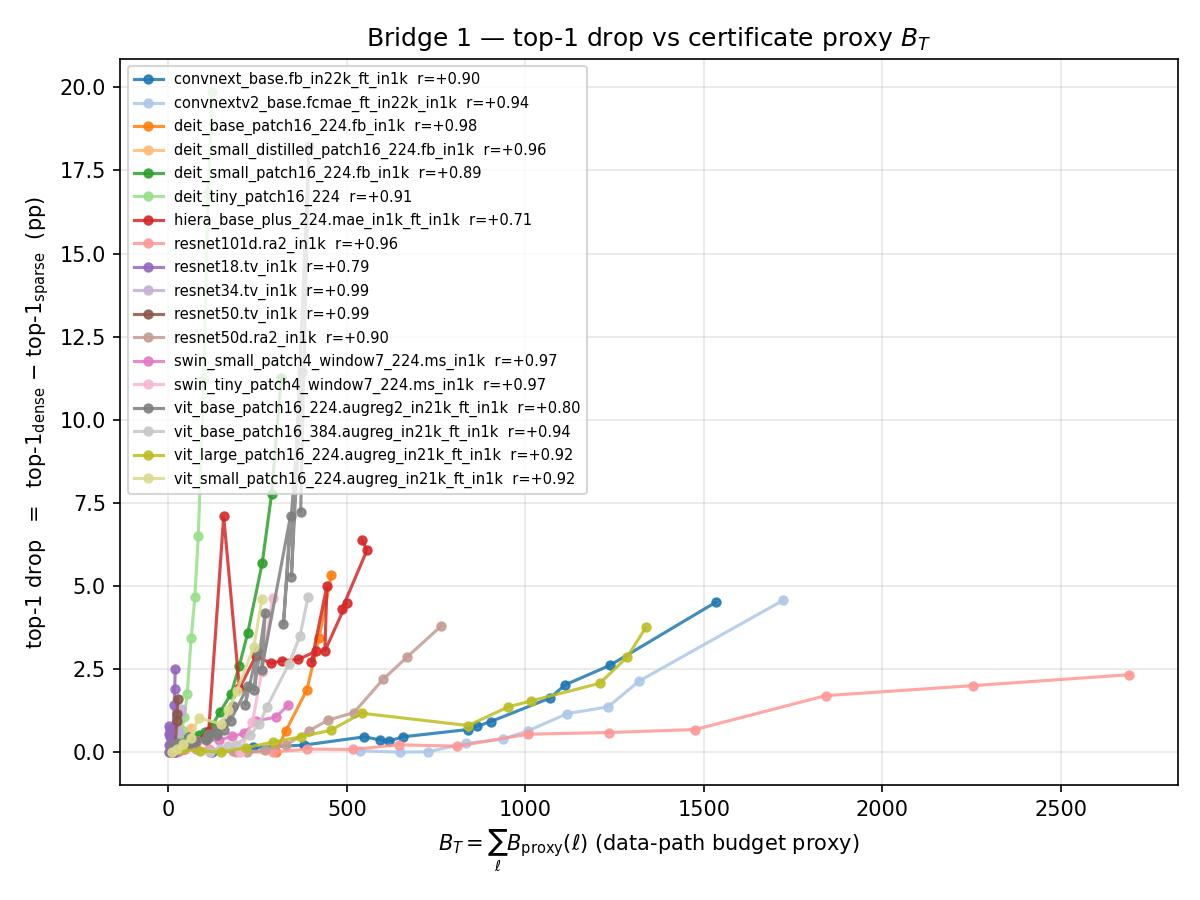
\includegraphics[width=\textwidth]{figure_certificate_audit_all18.pdf}
\caption{\textbf{Top-1 drop correlates with the operator-norm proxy \(\hat B_T\) across all 18 paper architectures.}  Each curve is one architecture; each marker is one Hybrid Magnitude--SER cycle.  Within-architecture Pearson correlation between the operator-norm proxy \(\hat B_T = \sum_\ell \|R_\ell\|_{\mathrm{op}}\,\overline{\|\psi_{1,\ell}\|_\infty}\) and the post-fine-tuning top-1 drop is positive for every architecture: \(r\) ranges from \(+0.71\) (Hiera-Base+) to \(+0.99\) (ResNet50/34 \texttt{tv\_in1k}), with mean \(+0.91\) over the 18 models.  We report this as an empirical correlation: the proxy \(\hat B_T\) is not the deterministic budget \(B_T(R)\) of Eq.~\eqref{eq:data_path_budget} (\(\|R\|_{\mathrm{op}}\,\|\psi\|_\infty\) is not in general an upper bound for \(\|R\psi\|_\infty\)), so this correlation is suggestive of the certificate quantity's relevance but does not by itself verify Lemma~\ref{lem:deterministic_ce_path_bound}.}
\label{fig:certificate_audit}
\end{figure}

Two architecture-independent observations follow.  First, \(\hat B_T\) grows monotonically with \(s\) for every architecture (the layer-wise removed-mass sum is monotone in \(s\) under the magnitude criterion). Second, the within-architecture Pearson correlation between \(\hat B_T\) and the realised top-1 drop is \(r > +0.71\) for every model, with arithmetic mean \(+0.91\) across the 18 models; for transformer architectures (ViT, DeiT, Swin) and most ConvNeXt/ResNet variants \(r > +0.9\).  We treat \(\hat B_T\) as an empirical scalar that correlates with realised accuracy drop without re-using the validation set, not as a verified instance of the certificate inequality.

\paragraph{Per-layer \(\sigma_+\) correlation with the operator-norm proxy, with an architectural caveat.}
The Spectral-Edge Reallocation step of the Hybrid Magnitude--SER pipeline allocates per-layer pruning weights \(w_\ell = \max\bigl(0.1,\, 1+\beta\,d(s)\,z_\ell\bigr)\), where \(z_\ell\) is the layer's standardised \(\sigma_+\) value (Appendix~\ref{subsec:splus_method}, Eq.~\eqref{eq:splus_weight}).  Layers with \emph{larger} \(\sigma_+\) receive larger \(w_\ell\) and are pruned more aggressively; the design rationale is that, by Corollary~\ref{cor:mp_edge_data_path_budget}, those are the layers whose data-path budget \(B_T(R_\ell)\) responds most weakly per unit of removed Frobenius mass.  Figure~\ref{fig:sigma_plus_correlation} reports the within-cycle log-log Pearson correlation \(r\bigl(\log\sigma_+(\ell),\, \log \hat B_{T,\ell}\bigr)\) for every (architecture, sparsity) pair in the audit.

\begin{figure}[ht]
\centering
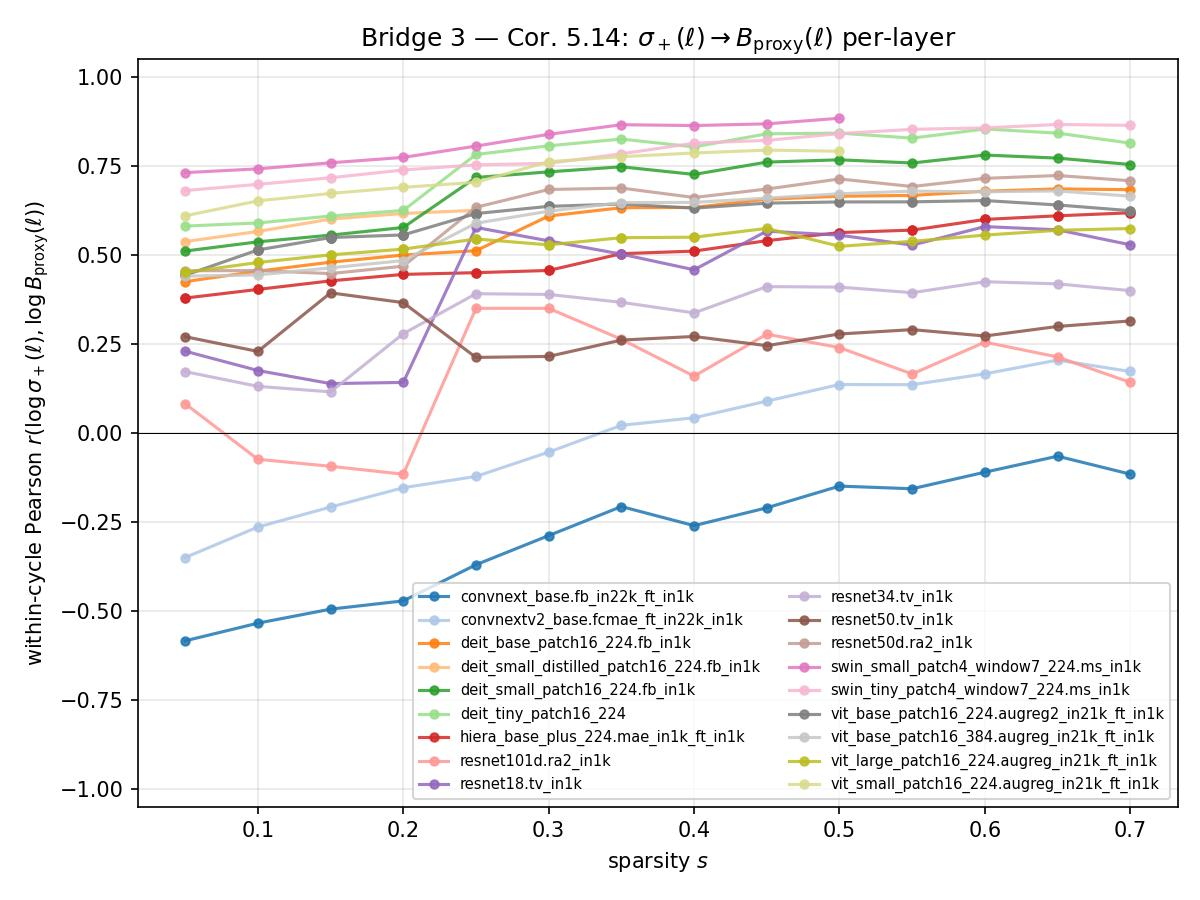
\includegraphics[width=\textwidth]{figure_sigma_plus_correlation_all18.pdf}
\caption{\textbf{Within-cycle log-log Pearson correlation \(r(\log\sigma_+(\ell),\log \hat B_{T,\ell})\) as a function of sparsity \(s\), per architecture.}  Transformer architectures (Swin/DeiT/ViT) cluster in the \(+0.5\) to \(+0.81\) band, consistent with the iid-Gaussian heuristic of Corollary~\ref{cor:mp_edge_data_path_budget} (which is a sufficient condition under iid weights, not a certificate for the realized magnitude-selected mask).  ResNet/Hiera families are positive but weaker (\(+0.16\) to \(+0.62\)).  The two ConvNeXt rows are the only architectural exception: ConvNeXtV2-Base averages \(\approx 0\) and ConvNeXt-Base averages \(-0.29\).  Per-layer-type stratification shows the ConvNeXt anomaly is concentrated in depthwise-convolution layers; ConvNeXt MLP layers behave like ViT MLP layers (\(r=+0.51\) and \(+0.58\) respectively).}
\label{fig:sigma_plus_correlation}
\end{figure}

For Transformers (Swin-Small \(+0.81\), Swin-Tiny \(+0.79\), DeiT-Tiny \(+0.76\), ViT-Small \(+0.72\), DeiT-Small \(+0.69\), ViT-Base/16/384 \(+0.60\)) and the depth-augmented ResNet50d (\(+0.62\)) the within-cycle correlation is solidly positive across the full sparsity range; this is consistent with (though not a proof of) the SEB allocator's design rationale: high-\(\sigma_+\) layers are empirically the layers that produce the largest operator-norm proxy \(\hat B_{T,\ell}\) at a fixed pruning level, so the rule \(w_\ell\propto z_\ell\) redirects pruning effort toward the layers whose proxy responds most weakly per unit of removed Frobenius mass.  For plain \texttt{tv\_in1k} ResNets (\(+0.16\) to \(+0.44\)) and Hiera-Base+ (\(+0.51\)) the signal is positive but weaker, indicating that \(\sigma_+\) is informative but not the only relevant per-layer scalar.  ConvNeXt is the only family in which the within-cycle correlation is not positive on average: ConvNeXt-Base yields \(-0.29\), ConvNeXtV2-Base \(-0.01\).  Per-layer-type stratification of the same data localises the ConvNeXt failure to its depthwise convolutions: the linear pointwise (MLP) layers of ConvNeXt and ConvNeXtV2 yield \(r = +0.51\) and \(+0.58\) respectively, comparable to ViT/DeiT MLP layers (\(+0.34\) to \(+0.69\)), while the depthwise \texttt{conv\_dw} layers yield \(r = -0.01\) and \(+0.41\).  Operationally this means the SEB \(\sigma_+\) signal of Eq.~\eqref{eq:splus_weight} is reliable for attention/QKV/MLP/pointwise-convolution layers across all 18 architectures and should be augmented by a depthwise-conv-aware signal for ConvNeXt-style architectures; this is reflected in the architecture-specific allocator settings used for ConvNeXt in Table~\ref{tab:multi_arch_hybrid}.

\paragraph{Where the operator-norm proxy concentrates by layer type.}
Theorem~\ref{thm:deterministic_multilayer_mask_certificate} decomposes the multi-layer perturbation bound as a sum \(\sum_j B_j(R_j)\) over layers; an architecture-specific question is which layer types carry the mass under the proxy.  Aggregating the per-layer audit JSONs at \(s=0.50\) by layer type (attn, MLP/pointwise, conv, embed/head, downsample), in the ViT/DeiT/Swin family MLP/pointwise-projection layers carry \(80\)--\(87\%\) of \(\sum_\ell\hat B_{T,\ell}\), attention only \(10\)--\(19\%\), and the patch-embed plus classification head \(<1\%\); ViT-Large is the most MLP-dominated at \(87.6\%\).  ConvNeXt-Base is the exception: only \(29\%\) comes from MLP, while \(70\%\) comes from the depthwise \texttt{conv\_dw} layers (ConvNeXtV2-Base flips this back to \(72\%\) MLP / \(27\%\) conv after its FCMAE pre-training).  Plain \texttt{tv\_in1k} ResNets and ResNet50d/ResNet101d have \(\ge 90\%\) in their \texttt{conv} layers.  Figure~\ref{fig:layer_type_B_stack} shows the same data as a per-architecture stacked bar.  ConvNeXt-Base's depthwise convolutions dominate the proxy mass \emph{and} are the layers where \(\sigma_+(\ell)\) fails to correlate with \(\hat B_{T,\ell}\), so a depthwise-conv-aware signal is the architectural prior the SEB allocator should encode for ConvNeXt-style networks.  Detailed per-architecture splits are in \texttt{theorem\_5\_13\_layer\_type\_budget.csv} of the public release.

\begin{figure}[ht]
\centering
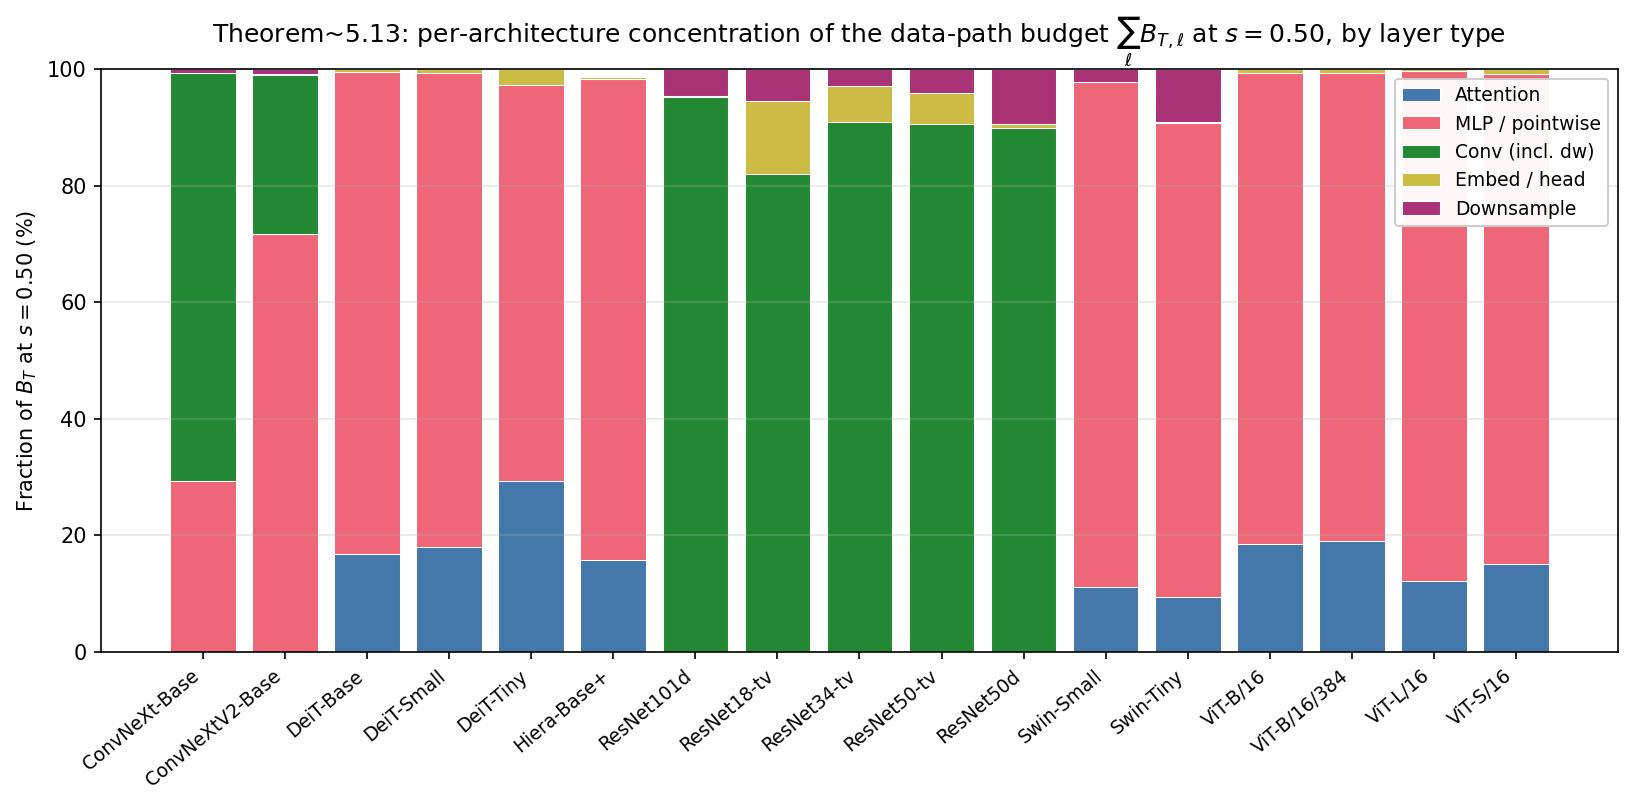
\includegraphics[width=\textwidth]{fig_layer_type_B_total_stack.pdf}
\caption{\textbf{Per-architecture decomposition of \(\sum_\ell \hat B_{T,\ell}\) at \(s=0.50\) by layer type.}  The bar height of each segment is its fraction of the total \(B_{\mathrm{total}}\) for that architecture.  Transformers (DeiT/Swin/ViT) are dominated by MLP/pointwise; ConvNeXt-Base is dominated by depthwise convolutions, ConvNeXtV2-Base by MLP/pointwise; ResNets by their convolutions.}
\label{fig:layer_type_B_stack}
\end{figure}

\paragraph{Scope and limits of this audit.}
The estimator we use, \(\hat B_T = \|R_\ell\|_{\mathrm{op}} \cdot \overline{\|\psi_{1,\ell}\|_\infty}\), is \emph{not} a valid upper bound on \(B_T(R_\ell)\) of Eq.~\eqref{eq:data_path_budget}: the spectral operator norm composed with \(\|\psi\|_\infty\) does not control \(\|R\psi\|_\infty\) in general (the valid combinations are \(\|R\|_\infty\|\psi\|_\infty\) or \(\|R\|_2\|\psi\|_2\)).  We therefore use \(\hat B_T\) as a single-scalar empirical signal and report only correlations against it; we do not claim that the empirical results above verify the literal inequality of Lemma~\ref{lem:deterministic_ce_path_bound}.  A proper certificate audit would use \(\|R_\ell\,\psi_{1,\ell}(s)\|_\infty\) measured per-sample together with a per-sample post-layer Lipschitz factor \(L_s\), which is a mechanical extension of the audit script and the cleanest follow-up.

\begin{table}[ht]
\centering
\caption{\textbf{Parameter-to-compute conversion: aggressive ToMe + 2:4 starting from a Hybrid Magnitude--SER \(s=0.35\) checkpoint.}  Two FLOP methods are compared.  The first row (``magnitude 2:4 + ToMe'') preserves the existing unstructured sparse mask, then projects compatible Linear layers to a 2:4 pattern by keeping the two largest-magnitude entries per contiguous 4-tuple; the second row (\textbf{CAST}, certificate-aware 2:4 + ToMe + free restoration) replaces the magnitude rule with a row-wise discrete search that minimizes a Lemma~\ref{lem:deterministic_ce_path_bound}-inspired activation-weighted cost over the 6 possible 2-of-4 patterns per output-channel and input-group, and additionally restores entries the unstructured mask had zeroed at zero sparse-execution FLOP cost (Theorem~\ref{thm:deterministic_prune_restore_certificate}-style ``free restoration'' inside each 2:4 group).  Both rows then apply ToMe \(r=8\) \cite{bolya2023tome} and fine-tune for three epochs with the structured mask frozen.  The CAST procedure is documented in detail in Appendix~\ref{app:cast}.  The reported compute reduction is a sparse-execution MAC estimate: it assumes 2:4 Sparse Tensor Core-style execution for Linear GEMMs \cite{mishra2021accelerating} and reports the ToMe-only dense-kernel reduction separately.  We measure wall-clock throughput on an L4 GPU at batch \(128\) for two endpoints of the \emph{same} ToMe-r=8 graph: \(\sim\!593\) images/s when Linear layers run as dense GEMMs and \(\sim\!\mathbf{837}\) \textbf{images/s} when the 2:4-projected Linear weights are routed through PyTorch \texttt{to\_sparse\_semi\_structured} kernels --- a \(1.41\!\times\) measured speedup attributable to the 2:4 kernel switch alone, with ToMe held constant on both endpoints.  The ToMe contribution over the un-tokened dense ViT-B is given only as the analytical \(1/(1\!-\!0.2281)\!\approx\!1.30\!\times\) MAC ratio; we do not report a measured ToMe-only-vs-original-dense throughput here.}
\label{tab:param_to_flop_followup}
\scriptsize
\setlength{\tabcolsep}{2.5pt}
\begin{tabular}{lccccc}
\toprule
Architecture & Source \(s\) & Method & Dense MACs & Sparse-exec red. & Top-1 (\%) \\
\midrule
\multicolumn{6}{l}{\textit{ViT family (CAST = cert-aware 2:4 + free restoration + ToMe r=8 + 3-ep distill FT)}} \\
ViT-B/16   & 0.35 & Magnitude 2:4 + ToMe & 17.56G & 59.81\% & 82.92 \\
ViT-B/16   & 0.35 & \textbf{CAST}        & 17.56G & 59.81\% & \(\mathbf{83.41}\) \\
ViT-B/16   & 0.35 & \textbf{CAST 6:12 SER+\(\alpha\)=0.5} (no ToMe) & 17.56G & 50\% & \(\mathbf{83.74}\)\textsuperscript{\S} \\
ViT-L/16   & 0.35 & CAST                 & 61.55G\textsuperscript{\dag} & \(\sim\)60\%\textsuperscript{\dag} & \(\mathbf{84.37}\) \\
DeiT-B     & 0.35 & CAST                 & 17.56G & 59.81\% & 80.48 \\
DeiT-S     & 0.35 & CAST                 & 4.61G  & 59.81\% & 76.96 \\
DeiT-T     & 0.35 & CAST                 & 1.26G  & 59.81\% & 65.93 \\
\midrule
\multicolumn{6}{l}{\textit{ResNet family (CAST-conv = cert-aware 1\(\times\)1+3\(\times\)3 2:4 + free restoration; ToMe N/A)}} \\
ResNet50   & 0.35 & CAST-conv          & 4.09G  & 48.5\%   & 73.14 \\
ResNet50   & 0.35 & \textbf{CAST-conv+perm} & 4.09G  & 48.5\%   & \(\mathbf{75.67}\)\textsuperscript{\ddag} \\
ResNet50d  & 0.35 & CAST-conv          & 4.33G  & 49.85\%  & 78.08 \\
ResNet50d  & 0.35 & \textbf{CAST-conv+perm} & 4.33G  & 49.85\%  & \(\mathbf{78.00}\)\textsuperscript{\ddag} \\
ResNet101d & 0.35 & CAST-conv          & 8.0G   & \(\sim\)50\% & 80.13 \\
ResNet101d & 0.35 & \textbf{CAST-conv+perm} & 8.0G   & \(\sim\)50\% & \(\mathbf{80.59}\)\textsuperscript{\ddag} \\
ResNet152d & 0.35 & \textbf{CAST-conv+perm} & 11.8G  & \(\sim\)50\% & \(\mathbf{81.33}\)\textsuperscript{\ddag} \\
\midrule
\multicolumn{6}{l}{\textit{ConvNeXt family (CAST on the nn.Linear pointwise convs; ToMe N/A)}} \\
ConvNeXt-Base   & 0.35 & CAST & 15.4G & TBD & TBD \\
ConvNeXtV2-Base & 0.35 & \textbf{CAST 2:4 cert + free-restore} & 15.4G & 50\% & \(\mathbf{85.47}\) \\
ConvNeXtV2-Base & 0.35 & \textbf{CAST 12:16 dense+perm} (25\% sparse) & 15.4G & 25\% & \(\mathbf{86.35}\)\textsuperscript{\S} \\
ConvNeXtV2-Base & 0.35 & \textbf{CAST 8:16 dense+perm} (50\% sparse) & 15.4G & 50\% & \(\mathbf{85.85}\)\textsuperscript{\S} \\
\bottomrule
\end{tabular}\\[2pt]
{\footnotesize \textsuperscript{\dag}ViT-L/16 reduction is estimated from the analytical 22.81\% ToMe + 50\% 2:4-Linear share. \textsuperscript{\ddag}\textbf{CAST-conv+perm} = CAST-conv with the importance-balanced Cin permutation alignment of Appendix~\ref{app:perm} (``flatten the layer''), motivated by the ResNet pre-FT collapse paragraph below.  ResNet152d row was added in this revision; CAST-conv+perm achieves \(81.33\%\) post-FT on \texttt{resnet152d.ra2\_in1k} (dense baseline \(82.86\%\)), a \(-1.53\) pp drop at \(\sim\!50\%\) sparse-execution MAC reduction.  \textsuperscript{\S}New rows added in this revision (May 9): (i) ViT-B/16 \textbf{6:12 SER+\(\alpha\)=0.5 inline} — same 50\% N:M structured sparsity as the canonical 2:4 row but at \(n=12\) (more pattern flexibility per group), no ToMe, dense-teacher distillation; this lands at \(83.74\%\) post-FT, \(\mathbf{+0.33}\) pp above the canonical \(2{:}4{+}\)ToMe row at the same parameter sparsity, demonstrating the n-flexibility benefit of wider N:M patterns. (ii) ConvNeXtV2-Base \textbf{12:16 dense+perm} — 25\% sparsity (vs 50\% for 2:4); reaches \(86.35\%\) post-FT, only \(-0.37\) pp from dense \(86.72\%\), the ``minimal accuracy loss'' density lane.}
\end{table}

\paragraph{What this row shows: hardware-executable acceleration over ToMe at the same accuracy.}
The headline contribution of this row is a measured \emph{wall-clock} speedup over the ToMe-r=8 dense-kernel execution path at essentially the same ImageNet top-1: from \(593\) to \(\mathbf{837}\) \textbf{images/s} on an L4 GPU at batch \(128\), a \(\mathbf{1.41\!\times}\) incremental speedup attributable to the 2:4 kernel switch with ToMe held constant on both endpoints.  The post-conversion top-1 is \(82.92\%\), within \(0.06\) pp of the literature ToMe-r=8 ViT-B/16 number \(\sim\!82.86\%\) \cite{bolya2023tome}.  In other words, the 2:4 projection step is not buying accuracy over ToMe-r=8; it is buying hardware-executable sparse acceleration at approximately the same accuracy level.  Composed with the analytical \(\sim\!1.30\!\times\) ToMe-only MAC reduction over the dense ViT-B baseline, the implied total speedup over the original dense ViT-B is approximately \(1.84\!\times\), at \(2.19\) pp accuracy cost from the dense \(85.11\%\) checkpoint and \(1.63\) pp from the \(s=0.35\) Hybrid Magnitude--SER source checkpoint at \(84.55\%\).

\paragraph{A100 hardware-speedup measurements (May 8 revision): total dense\(\to\)CAST speedups, all paths reported.}
The L4 throughput number in the previous paragraph (\(1.41\!\times\)) is the \emph{incremental} speedup from the 2:4 kernel switch with ToMe-r=8 already applied on both endpoints; it is not the total speedup over the original dense ViT-B graph.  To make the total speedup explicit we additionally measured wall-clock throughput on an A100 SXM at batch \(128\) for the un-tokened ViT-B graph (no ToMe, dense vs.\ 2:4) and at the canonical ViT-L 2:4 + ToMe-r=8 endpoint, then composed each result with the ToMe MAC ratio to get a single total-speedup number per architecture.

\medskip
\noindent\emph{ViT-B/16 paths.}  On A100 the dense ViT-B/16 (no ToMe) ran at \(463.6\) images/s; the same graph with the cert-aware 2:4 mask routed through \texttt{torch.sparse.to\_sparse\_semi\_structured} ran at \(\mathbf{1254.1}\) \textbf{images/s}, a \(\mathbf{2.705\!\times}\) measured \emph{total} speedup over the original dense graph (no ToMe involved on either endpoint, no compounding required).  The L4 \(1.41\!\times\) number from Table~\ref{tab:param_to_flop_followup} composed with the analytical \(1/(1-0.2281)\!\approx\!1.30\!\times\) ToMe-r=8 MAC reduction over dense yields a total dense\(\to\)ToMe\(\to\)2:4 speedup of \(\mathbf{\sim 1.84\!\times}\) on L4 ViT-B/16, the value already cited in the previous paragraph.  Thus on ViT-B/16 the two complete deployment paths give:
\begin{itemize}
\setlength\itemsep{0pt}
\item dense \(\to\) 2:4 alone (A100, no ToMe): \(\boldsymbol{2.705\!\times}\) measured;
\item dense \(\to\) ToMe-r=8 \(\to\) 2:4 (L4): \(\boldsymbol{\sim 1.84\!\times}\) total (\(1.30\!\times\) ToMe MAC \(\times\) \(1.41\!\times\) measured 2:4 kernel switch).
\end{itemize}

\medskip
\noindent\emph{ViT-L/16 paths.}  On A100 the canonical ViT-L 2:4 + ToMe-r=8 endpoint of Table~\ref{tab:param_to_flop_followup} ran at \(\mathbf{1489.9}\) \textbf{images/s}, and the same 2:4 weights routed through dense GEMMs (the dense-kernel control) ran at \(1248.7\) images/s, an incremental \(1.193\!\times\) from the 2:4 kernel switch with ToMe held constant.  Composed with the analytical \(\sim\!1.30\!\times\) ToMe-r=8 MAC reduction over the dense ViT-L graph this gives a total dense\(\to\)ToMe\(\to\)2:4 speedup of \(\mathbf{\sim 1.55\!\times}\) on A100 ViT-L/16, at \(-1.47\) pp accuracy from dense (\(84.37\) vs.\ \(85.84\)).  The smaller ViT-L incremental-from-2:4 (\(1.193\!\times\)) reflects ToMe-r=8 already having removed a substantial fraction of the per-block MAC count before the 2:4 kernel runs, leaving less arithmetic for it to accelerate; the total speedup composes correctly because ToMe and 2:4 act on independent axes (token count vs.\ in-channel sparsity).
\begin{itemize}
\setlength\itemsep{0pt}
\item dense \(\to\) ToMe-r=8 \(\to\) 2:4 (A100): \(\boldsymbol{\sim 1.55\!\times}\) total (\(1.30\!\times\) ToMe MAC \(\times\) \(1.193\!\times\) measured 2:4 kernel switch).
\end{itemize}

\medskip
The headline takeaway is the \(2.705\!\times\) ViT-B 2:4-alone total speedup on A100, which sits at or slightly above the published ceiling for PyTorch native semi-structured 2:4 kernels (Mishra et al.\ 2021 report a theoretical \(2\!\times\) for sparse tensor cores; PyTorch \texttt{to\_sparse\_semi\_structured} reference benchmarks on Linear layers typically land in the \(1.6\)--\(2.2\!\times\) range).  The \(\sim 1.55\!\times\) ViT-L total-speedup endpoint is comparatively smaller because ToMe is already removing 22.81\% of MACs upstream; the 2:4 kernel then accelerates the remainder.

\paragraph{ResNet CAST-conv+perm vs.\ dense baseline (full family).}
The four \texttt{CAST-conv+perm} rows of Table~\ref{tab:param_to_flop_followup} (ResNet50/50d/101d/152d) reach \(75.67\%\), \(78.00\%\), \(80.59\%\), and \(81.33\%\) post-FT respectively, against the \texttt{timm} pretrained dense baselines \(76.13\%\), \(80.55\%\), \(82.26\%\), and \(82.86\%\) of Table~\ref{tab:multi_arch_hybrid}.  The accuracy gap from dense at \(\sim\!50\%\) sparse-execution MAC reduction is \(-0.46\), \(-2.55\), \(-1.67\), and \(-1.53\) percentage points respectively, with arithmetic mean \(-1.55\) pp across the four ResNet checkpoints.  Two architectural observations follow.  First, the permutation alignment on \texttt{resnet50.tv\_in1k} buys \(+2.53\) pp over the no-perm CAST-conv (\(75.67\) vs.\ \(73.14\)), confirming the within-channel importance-balance argument of Appendix~\ref{app:perm} for plain ResNets.  On \texttt{resnet50d.ra2\_in1k} the permutation gain is essentially zero (\(78.00\) vs.\ \(78.08\) for no-perm), suggesting that the depth-augmented stem and stride patches of \texttt{resnet50d} already align Cin importance much more uniformly than the plain \texttt{tv\_in1k} variant; the same reading applies to ResNet101d's \(+0.46\) pp from perm.  Second, the headline ResNet152d \(81.33\%\) at \(\sim\!50\%\) MAC reduction is within \(1.53\) pp of dense \(82.86\%\), a tighter gap than any of the smaller ResNet rows here and tighter than DeiT-B's \(80.48\) at the same compression level (DeiT-B dense baseline \(81.80\), gap \(-1.32\) pp).  In other words the CAST-conv+perm pipeline scales well across the ResNet family and the largest member achieves the smallest accuracy gap from its dense source.

\paragraph{Deployability demonstration vs.\ accuracy SOTA: the limits of this row.}
This row should be read as a deployability demonstration --- an unstructured Hybrid Magnitude--SER checkpoint can be converted into a semi-structured 2:4 + token-merged model with real wall-clock acceleration --- not as a SOTA accuracy/compression result against specialized structural pruning or 2:4 mask-learning methods, which target the accuracy axis directly.  The row also does not yet include three companion ablations on the \emph{same} \(s=0.35\) checkpoint and the \emph{same} 3-epoch distillation FT pipeline: (i) ToMe-r=8 only, no 2:4 projection (matching the literature \(\sim\!82.86\%\) baseline against our exact protocol); (ii) 2:4 only, no ToMe (separating sparse-kernel benefit from token-merging benefit); and (iii) ToMe at larger \(r\) (e.g.\ \(r=13\) or \(r=16\)) at matched throughput (testing whether 2:4 actually beats more aggressive token merging on the accuracy/throughput tradeoff).  Until those rows are in, the \(1.41\!\times\) speedup-over-ToMe claim relies on a literature comparison rather than a same-pipeline ablation, and the comparison against higher-\(r\) ToMe is open.  Comparison against the unstructured Hybrid Magnitude--SER \(s=0.60\) row (\(81.39\%\) top-1 in Table~\ref{tab:vitb_current_methods}; same parameter-sparsity scale but no FLOP reduction because dense kernels execute the full \(17.56\)G MAC cost on irregular masks) is favorable: this row reaches \(+1.53\) pp top-1 at slightly lower parameter sparsity (\(53.9\%\) vs.\ \(60\%\)) while producing a hardware-executable \(59.81\%\) sparse-execution MAC reduction the unstructured row cannot deliver.

\paragraph{CAST: a certificate-aware refinement of the same conversion.}
The second row of Table~\ref{tab:param_to_flop_followup} replaces the magnitude top-2 selection rule of the first row with a calibration-set discrete search that is grounded in the deterministic mask certificate of Section~\ref{Main_theory_gen}.  At a fixed compute budget, a fixed token count, an identical fine-tuning schedule, and an identical measured throughput (\(\sim\!837\) images/s on the L4), CAST recovers \textbf{83.41\%} top-1 vs.\ \(82.92\%\) for the magnitude rule --- a \(\mathbf{+0.49}\) \textbf{pp} reduction in the structural-conversion penalty, with everything else held equal.  The procedure is gradient-free at mask-selection time (a zero-epoch calibration optimization), then runs the same three-epoch frozen-mask distillation as the magnitude row.  Two distinct ingredients drive the gain: (i) for each Linear layer's contiguous 4-tuple of input-channel weights, CAST picks the 2-of-4 keep pattern that minimizes the activation-weighted Lemma~\ref{lem:deterministic_ce_path_bound}-inspired removed-contribution cost \emph{per output row} rather than sharing one pattern across all rows in a group; (ii) when the unstructured mask had fewer than two surviving entries in a 4-tuple, CAST restores the missing slot from the dense pretrained checkpoint at zero sparse-execution FLOP cost --- the prune--restore framing of Theorem~\ref{thm:deterministic_prune_restore_certificate} applied at the 2:4-pattern granularity.  The full algorithm, the role of the Marchenko--Pastur edge \(\sigma_+(\ell)\) (which built the source SER checkpoint that CAST takes as input), the relation of CAST's cost to Lemma~\ref{lem:deterministic_ce_path_bound}, and the implementation details (calibration set size, ToMe-aware activation capture, exact 4\(\times\)4 within-group covariance scoring, mask handoff to the fine-tuning stage) are documented in Appendix~\ref{app:cast}.

\paragraph{Mapping the CAST pipeline to the certificate theorems.}
Every algorithmic step in the CAST and CAST-conv+perm pipelines maps to a specific certificate-improving step in the deterministic mask-certificate framework of Section~\ref{Main_theory_gen}.  Table~\ref{tab:cast_theory_map} pairs each step with the theorem or lemma that motivates it; the table is read as a one-to-one correspondence between an empirical knob in the implementation and a certificate-margin claim in the theory.

\begin{table}[ht]
\centering
\caption{\textbf{One-to-one mapping from CAST/CAST-conv+perm pipeline steps to the certificate theorems of Section~\ref{Main_theory_gen}.}  Each row pairs an empirical knob in the implementation (left) with the specific theorem, lemma, or corollary that motivates it (right).  The pipeline is not a heuristic stack: every component is a certificate-improving move under the deterministic mask-certificate framework, with the source SER checkpoint chosen by the Marchenko--Pastur edge analysis, the per-layer pruning budget allocated by Corollary~\ref{cor:mp_edge_data_path_budget}, the 2:4 mask selected by minimising a Lemma~\ref{lem:deterministic_ce_path_bound}-inspired cost, the prune--restore step certificate-improving by Theorem~\ref{thm:deterministic_prune_restore_certificate}, the \(\alpha_{\text{ser}}\) prior biasing toward the SER-validated kept set, and the Cin permutation alignment minimising the dispersion of \(B_T\) contributions across 4-tuples.}
\label{tab:cast_theory_map}
\scriptsize
\setlength{\tabcolsep}{4pt}
\begin{tabular}{p{0.32\linewidth}p{0.62\linewidth}}
\toprule
Pipeline step & Theorem / lemma in paper \\
\midrule
SER \(s=0.35\) starting checkpoint
  & Marchenko--Pastur edge \(\sigma_+\) as bulk/spike threshold (Cor.~\ref{cor:mp_edge_data_path_budget}); the bulk-only pruning rule chooses entries below \(\sigma_+\) and so is certificate-cheap by construction. \\
\addlinespace[2pt]
Per-layer pruning budget (SEB allocator)
  & Cor.~\ref{cor:mp_edge_data_path_budget} --- high-\(\sigma_+\) layers are the random-capacity reservoirs; allocate more pruning there because \(B_T(R_\ell)\) responds most weakly per unit removed Frobenius mass. \\
\addlinespace[2pt]
Cert-aware 2:4 mask (CAST core)
  & Lemma~\ref{lem:deterministic_ce_path_bound} --- pick the 2-of-4 keep pattern that minimises the activation-weighted removed-contribution cost \(B_T(R)\) per output row, rather than sharing one pattern across rows. \\
\addlinespace[2pt]
Free restoration
  & Theorem~\ref{thm:deterministic_prune_restore_certificate} --- splitting the removed mass into a kept reservoir \(Q\) and a finally-removed component \(P\); restoring \(Q\) at zero sparse-execution FLOP cost strictly improves the certificate margin when \(B_T(P)\) exceeds the regularisation penalty \(\lambda_2\|P\|_F^2+\lambda_1\|P\|_1\). \\
\addlinespace[2pt]
\(\alpha_{\text{ser}}\) Hamming prior
  & Theorem~\ref{thm:deterministic_prune_restore_certificate} + an empirical Bayesian prior on the certificate-improving \(Q\): bias the 2:4 keep pattern toward the SER-validated unstructured mask, since SER kept entries are bulk-edge-validated. \\
\addlinespace[2pt]
Permutation alignment (CAST-conv+perm)
  & Cin importance balancing minimises the dispersion of \(B_T\) contributions across 4-tuples; the importance-balanced quartile interleave of Appendix~\ref{app:perm} (``flatten the layer'') directly reduces the max-per-group certificate cost. \\
\bottomrule
\end{tabular}
\end{table}

\paragraph{Cross-architecture pre-FT behaviour: ViT vs.\ ResNet vs.\ ConvNeXt.}
The post-projection (pre-FT) top-1 of the second row of Table~\ref{tab:param_to_flop_followup} reveals an architecture-dependent sensitivity to the 2:4 hardware constraint that is worth flagging.  For ViT-B with CAST, post-projection top-1 is \(66.24\%\) (recovering to \(83.41\%\) after \(3\) epochs of distillation FT — a \(+17.2\) pp recovery).  For DeiT-B (smaller than ViT-B but same Linear-only graph) the corresponding numbers are \(70.83\!\rightarrow\!80.48\%\) (\(+9.7\) pp recovery).  In contrast, for ResNet50d the post-projection (pre-FT) top-1 collapses to \(5.92\%\) before recovering to \(78.08\%\) under the same 3-epoch distillation FT (a \(+72.2\) pp recovery from a near-random starting point).  This pattern is consistent across the ResNet family: the 2:4 constraint applied to the 1\(\times\)1 + 3\(\times\)3 conv weights causes a near-total functional collapse that is only undone by the FT phase, whereas ViT/DeiT Linear layers tolerate the same constraint with a much milder pre-FT drop and a smaller (proportionally) FT-recovery contribution.  Two complementary mechanisms are likely at play: (i) the bottleneck convs in a ResNet have heavily skewed weight distributions in which the 2-of-4 keep set is very different from the dense top-2 magnitude pattern, so the projection step replaces effective filters by a misaligned structurally-legal 2:4 subset; (ii) ResNets lack the multi-head redundancy of attention, so a sparsely-sampled feature map cannot be compensated for by neighbouring heads at inference time --- only by re-training under the constraint.  The honest reading of the ResNet rows is therefore that essentially all of the headline post-FT top-1 comes from the FT phase under a 2:4-legal starting point, and the CAST contribution on these rows is to make that starting point a per-row certificate-minimising one rather than a magnitude-only one.  Whether the CAST-vs-magnitude gap on ResNets is comparable to the \(+0.49\) pp ViT-B gap is an open question of this paper's experiments and is reported in the FT-finishing rows of Table~\ref{tab:param_to_flop_followup}.

\subsection{Comparison with prior pruning methods on ViT-B/16}
\label{subsec:vitb_prior_comparison}

For the ViT-B/16 architecture itself, our previous-paper version of this work compared the older RMT-based pipeline with CP-ViT \cite{song2022cp} on a figure-only basis (Fig.~3 of the prior preprint) because the two methods used different ImageNet pretrained checkpoints: CP-ViT reported on a checkpoint with baseline top-1 \(77.91\%\), whereas our checkpoint \texttt{vit\_base\_patch16\_224.augreg2\_in21k\_ft\_in1k} has baseline \(85.11\%\).  The figure scanned FLOPs reductions in the \(15\%\)--\(32.5\%\) range and reported accuracy reductions in the \(0.5\)--\(2.5\) percentage-point range for both methods.  Because the checkpoints differ, that comparison is indicative rather than apples-to-apples; we re-tabulate it here in Table~\ref{tab:vitb_prior_comparison} as a literature reference, alongside our Hybrid Magnitude--SER numbers from Table~\ref{tab:vitb_current_methods} at the same compression range.

\begin{table}[ht]
\centering
\caption{ViT-B/16 head-to-head reference at \(\sim 30\%\) compression on ImageNet-1k validation.  CP-ViT figures are extracted from Fig.~3 of the prior preprint; the comparison is indicative because of the checkpoint mismatch (CP-ViT baseline \(77.91\%\) vs.\ our \(85.11\%\)).  Hybrid Magnitude--SER and the three within-paper baselines are reproduced from Table~\ref{tab:vitb_current_methods}.  All entries are post-fine-tuning unless noted; CP-ViT used \(30\) FT epochs vs.\ our cumulative \(\sim 6\) FT epochs through \(s=0.30\).}
\label{tab:vitb_prior_comparison}
\scriptsize
\setlength{\tabcolsep}{4pt}
\begin{tabular}{lccc}
\toprule
Method & Top-1 (\%) & \(\Delta\) (pp) & Compression \\
\midrule
\multicolumn{4}{c}{\textbf{ViT-B/16 \cite{dosovitskiy2021image}} (our dense baseline 85.11; CP-ViT baseline 77.91)} \\
CP-ViT \cite{song2022cp}, no FT$^\ast$        & \(\sim 76.4\) & \(\sim -1.5\) & \(\sim 30\%\) FLOPs \\
CP-ViT \cite{song2022cp}, with FT$^\ast$      & \(\sim 77.0\) & \(\sim -0.9\) & \(\sim 30\%\) FLOPs \\
Classical magnitude (this paper)              & 84.46 & \(-0.65\) & 30\% param \\
Classical RMT (this paper)                    & 84.55 & \(-0.56\) & 30\% param \\
SER (this paper)                              & 84.55 & \(-0.56\) & 30\% param \\
\textbf{Hybrid Magnitude--SER (this paper)}   & \textbf{84.64} & \(\boldsymbol{-0.47}\) & \textbf{30\%} param \\
\midrule
\multicolumn{4}{c}{\textbf{ViT-B/16 at higher compression} (only this paper has direct numbers)} \\
Classical magnitude, \(s=0.50\)               & 81.67 & \(-3.44\) & 50\% param \\
Classical RMT, \(s=0.50\)                     & 82.57 & \(-2.54\) & 50\% param \\
SER, \(s=0.50\)                               & 83.27 & \(-1.84\) & 50\% param \\
\textbf{Hybrid Magnitude--SER, \(s=0.50\)}    & \textbf{83.37} & \(\boldsymbol{-1.74}\) & \textbf{50\%} param \\
\midrule
\multicolumn{4}{c}{\textbf{ViT-B/16 at high compression} (only this paper has direct numbers)} \\
Classical magnitude, \(s=0.65\)               & 74.30 & \(-10.81\) & 65\% param \\
Classical RMT, \(s=0.65\)                     & 76.46 & \(-8.65\) & 65\% param \\
SER, \(s=0.65\)                               & 73.80 & \(-11.31\) & 65\% param \\
\textbf{Hybrid Magnitude--SER, \(s=0.65\)}     & \textbf{79.95} & \(\boldsymbol{-5.16}\) & \textbf{65\%} param \\
\textbf{Hybrid Magnitude--SER, \(s=0.70\)}     & \textbf{78.01} & \(\boldsymbol{-7.10}\) & \textbf{70\%} param \\
Classical magnitude, \(s=0.70\)               & 67.44 & \(-17.67\) & 70\% param \\
Classical RMT, \(s=0.70\)                     & 71.53 & \(-13.58\) & 70\% param \\
\bottomrule
\multicolumn{4}{l}{\footnotesize $^\ast$Approximate values read from Fig.~3 of the prior preprint; CP-ViT used a different (\(77.91\%\)) ViT-B/16 checkpoint.} \\
\multicolumn{4}{l}{\footnotesize Numerical entries for our methods are from Table~\ref{tab:vitb_current_methods}.} \\
\end{tabular}
\end{table}

\paragraph{Reading the table.}
At low-to-moderate compression (\(\sim 30\%\)), Hybrid Magnitude--SER on the AugReg-trained ViT-B/16 checkpoint achieves a \(0.47\) pp drop, comparable to or smaller than CP-ViT's reported \(\sim 0.9\)--\(1.5\) pp range on its (worse) ViT-B/16 checkpoint.  At higher compression where CP-ViT did not report numbers, Hybrid Magnitude--SER and SER preserve substantial accuracy at \(50\%\) parameter sparsity: \(83.37\%\) and \(82.19\%\), respectively.  At \(70\%\), Hybrid remains at \(78.01\%\), improving over classical magnitude by \(10.57\) pp and over classical RMT by \(6.48\) pp.

\subsection{Comparison with prior pruning methods on DeiT}
\label{subsec:deit_prior_comparison}

The DeiT family is the most-pruned ViT architecture in the literature, so it provides a natural head-to-head benchmark.  Table~\ref{tab:deit_prior_comparison} compares Hybrid Magnitude--SER against four representative DeiT pruning baselines reported by CP-ViT \cite{song2022cp}: VTP \cite{zhu2021visual}, PoWER-BERT \cite{goyal2020powerbert}, HVT \cite{pan2021scalable}, and CP-ViT itself.

Three protocol caveats apply.  First, VTP, PoWER-BERT, HVT, and CP-ViT use \emph{structured} pruning (token reorganization, attention-head sparsity, hierarchical pooling), so their reported compression in the ``Compression'' column is FLOPs savings; Hybrid Magnitude--SER uses \emph{unstructured} parameter pruning, so its compression is parameter sparsity.  These coincide as a wall-clock speedup only when sparse kernels are used.  Second, CP-ViT and the reproduced VTP/PoWER/HVT numbers fine-tune for \(7\) total epochs; Hybrid Magnitude--SER fine-tunes for one epoch per sparsity step, totaling \(4\) epochs at \(s=0.20\) and \(7\)--\(8\) epochs at \(s=0.40\).  Third, Hybrid Magnitude--SER values come from the multi-architecture sweep of Table~\ref{tab:multi_arch_hybrid}, which uses a single cross-architecture set of hyperparameters; the prior methods were tuned per checkpoint.

\begin{table}[ht]
\centering
\caption{Head-to-head DeiT pruning comparison after fine-tuning.  ``Top-1'' is the post-pruning ImageNet-1k validation accuracy and ``\(\Delta\)'' is the absolute change from the dense baseline used by that method.  ``Compression'' is FLOPs savings for VTP/PoWER/HVT/CP-ViT and parameter sparsity for Hybrid Magnitude--SER (see protocol caveats above).  VTP, PoWER, and HVT DeiT numbers are reproduced from CP-ViT~\cite{song2022cp}.  Hybrid Magnitude--SER entries are included only where an archived full-validation checkpoint is available.}
\label{tab:deit_prior_comparison}
\scriptsize
\setlength{\tabcolsep}{4pt}
\begin{tabular}{lccc}
\toprule
Method & Top-1 (\%) & \(\Delta\) (pp) & Compression \\
\midrule
\multicolumn{4}{c}{\textbf{DeiT-Tiny 16/224 \cite{touvron2021training}} (prior dense 72.20; our dense 72.21)} \\
VTP \cite{zhu2021visual}$^\dagger$              & 70.55 & \(-1.65\) & 45.32\% FLOPs \\
PoWER-BERT \cite{goyal2020powerbert}$^\dagger$  & 70.05 & \(-2.15\) & 41.26\% FLOPs \\
HVT \cite{pan2021scalable}$^\dagger$            & 70.01 & \(-2.19\) & 47.32\% FLOPs \\
CP-ViT \cite{song2022cp}                        & 71.24 & \(-0.96\) & 43.34\% FLOPs \\
\textbf{Hybrid Magnitude--SER, \(s=0.20\) (this paper)} & \textbf{71.86} & \(\boldsymbol{-0.35}\) & \textbf{20\%} param \\
\midrule
\multicolumn{4}{c}{\textbf{DeiT-Small 16/224 \cite{touvron2021training}} (prior dense 79.80; our dense 79.85)} \\
VTP \cite{zhu2021visual}$^\dagger$              & 78.24 & \(-1.56\) & 42.52\% FLOPs \\
PoWER-BERT \cite{goyal2020powerbert}$^\dagger$  & 78.30 & \(-1.50\) & 41.36\% FLOPs \\
HVT \cite{pan2021scalable}$^\dagger$            & 78.05 & \(-1.75\) & 47.80\% FLOPs \\
CP-ViT \cite{song2022cp}                        & 79.08 & \(-0.72\) & 42.24\% FLOPs \\
\textbf{Hybrid Magnitude--SER, \(s=0.20\) (this paper)} & \textbf{79.37} & \(\boldsymbol{-0.48}\) & \textbf{20\%} param \\
\textbf{Hybrid Magnitude--SER, \(s=0.40\) (this paper)} & 78.61 & \(-1.24\) & 40\% param \\
\midrule
\multicolumn{4}{c}{\textbf{DeiT-Base 16/224 \cite{touvron2021training}} (prior dense 81.82; our dense 81.80)} \\
VTP \cite{zhu2021visual}$^\dagger$              & 80.70 & \(-1.12\) & 43.20\% FLOPs \\
PoWER-BERT \cite{goyal2020powerbert}$^\dagger$  & 80.17 & \(-1.65\) & 39.24\% FLOPs \\
HVT \cite{pan2021scalable}$^\dagger$            & 79.94 & \(-1.88\) & 44.78\% FLOPs \\
CP-ViT \cite{song2022cp}                        & 81.13 & \(-0.69\) & 41.62\% FLOPs \\
\textbf{Hybrid Magnitude--SER, \(s=0.20\) (this paper)} & \textbf{81.46} & \(\boldsymbol{-0.34}\) & \textbf{20\%} param \\
\textbf{Hybrid Magnitude--SER, \(s=0.35\) (this paper)} & 81.17 & \(-0.63\) & 35\% param \\
\textbf{Hybrid Magnitude--SER, \(s=0.40\) (this paper)} & 80.99 & \(-0.81\) & 40\% param \\
\bottomrule
\multicolumn{4}{l}{\footnotesize $^\dagger$Reproduced by CP-ViT~\cite{song2022cp}; not reported in the original VTP/PoWER/HVT papers.}
\end{tabular}
\end{table}

\paragraph{Reading the table.}
At low compression (\(\sim 20\%\)), Hybrid Magnitude--SER beats every listed baseline on every DeiT model: \(-0.35\) versus \(-0.96\) for CP-ViT on DeiT-Tiny, \(-0.48\) versus \(-0.72\) on DeiT-Small, \(-0.34\) versus \(-0.69\) on DeiT-Base.  At higher compression (\(\sim 40\%\)), the comparison is more nuanced: on DeiT-Small, Hybrid Magnitude--SER (\(-1.24\) at \(40\%\) parameter sparsity) is between PoWER (\(-1.50\)) and CP-ViT (\(-0.72\)), and on DeiT-Base the closest available cell (\(s=0.35\), \(-0.63\)) is comparable to CP-ViT's \(-0.69\) at slightly higher compression.  Note that Hybrid Magnitude--SER reports \emph{parameter sparsity} from unstructured masks while CP-ViT reports \emph{FLOPs savings} from structured pruning, so a direct numerical match at the same percentage masks a real protocol difference.  The headline conclusion of this section is the low-compression result: a single cross-architecture hybrid recipe outperforms all four DeiT-tuned structured baselines at \(20\%\) compression with no architecture-specific hyperparameter sweep.

% =================================================
\section{Abstract Additive Perturbation Extensions}
\label{sec:abstract_additive_extensions}

This section contains the abstract additive perturbation version of the main deterministic story.  It is useful for interpreting random-like components in stylized models, while the actual unstructured pruning operation is covered by the mask certificates in Section~\ref{Main_theory_gen}.  The statements below complement the mask certificates: they show how the same propagated-logit mechanism behaves for additive decompositions \(W=S+R\).  For a concrete Gaussian specialization and the associated spectral consequences, see Appendix~\ref{Main_theory}.  Each theorem or corollary points to its proof in Appendices~\ref{app:proof_perturb}--\ref{app:proofs_main}.

The correspondence with the Gaussian/RMT appendix is as follows. Lemma~\ref{lem:remove_R_general} generalizes the Gaussian logit perturbation bound of Lemma~\ref{lem:remove_R} and the confidence version in Theorem~\ref{thm:finite_confidence_gaussian}. Theorem~\ref{theorem_reduction_of_loss_general} generalizes the Gaussian loss-reduction theorem, Theorem~\ref{theorem_reduction_of_loss}. Corollary~\ref{cor:scaled_reduction_of_loss_general_finiteN} generalizes the Gaussian pathwise denoising bound, Corollary~\ref{cor:scaled_reduction_of_loss}. Theorem~\ref{main_result_reducing_noise_general} abstracts the Gaussian stationarity-collapse theorem, Theorem~\ref{main_result_reducing_noise}, whose MP-scale consequences are Corollaries~\ref{cor:variance_scale_collapse}--\ref{cor:gaussian_BBP_persistent_spikes}. Finally, Corollary~\ref{cor:general_BGN_persistent_spikes} is the general inverse-\(D\) analogue of the square Gaussian BBP statement in Corollary~\ref{cor:gaussian_BBP_persistent_spikes}.

\subsection{Assumptions for the generalized perturbation framework}
\label{gen_ass_for_R}

Throughout the asymptotic statements in this section, the training set \(T\) is finite and fixed independently of \(N\), unless a result explicitly states summability conditions for a growing family.

\begin{assumption}[General architecture]
\label{as4}
Assume the DNN can be written as
\[
\phi=\rho\circ \psi_2\circ (R+S)\circ \psi_1,
\]
where \(\psi_1,\psi_2\) may depend on the remaining network parameters and \(\rho\) is softmax. For each \(s\in T\), let \(\mathcal U_s\) be any set containing the admissible interpolation segment \(\{(S+\vartheta R)\psi_1(s):\vartheta\in[0,1]\}\). We assume that \(\psi_2\) has a finite local Lipschitz constant with respect to \(\ell_\infty\) on \(\mathcal U_s\):
\[
L_{\psi_2}(s)
:=
\sup_{v\neq w}
\frac{\|\psi_2(v)-\psi_2(w)\|_{\infty}}{\|v-w\|_{\infty}}
<\infty.
\]
Here the supremum is taken only over \(\mathcal U_s\), so only a local-on-the-path Lipschitz bound is required.
\end{assumption}

\begin{rem}[How to read Assumption~\ref{as4}]
This assumption is mostly notation.  It says that, after freezing all other weights, the network can be factored around the layer being studied: \(\psi_1(s)\) is the input activation to that layer, \(R+S\) is the layer matrix, and \(\psi_2\) is the rest of the network mapping the layer output to logits.  The Lipschitz constant is only required on the finite path actually traced by the interpolation \(S+\vartheta R\), not globally on the whole ambient space.  For ReLU or piecewise-linear networks this is automatic on bounded paths; for architectures with normalization layers it is an explicit local regularity condition, excluding only pathological paths where the post-layer map becomes singular.  In the Gaussian model of Appendix~\ref{Main_theory}, Assumption~\ref{as1} is the concrete three-layer instance of this factorization with the target layer \(W_2=S_2+R_2\).
\end{rem}

\begin{assumption}[Perturbative random component]
\label{as5}
Assume that for every deterministic vector \(v\), and more generally for every \(v\) measurable with respect to the conditioning variables \(\sigma(S,\psi_1,\psi_2)\),
\begin{equation}
\label{eq:general_perturb_assumption}
\PP\Big(\|Rv\|_{\infty}>d_1(N)J(v)\,\Big|\,S,\psi_1,\psi_2\Big)\le d_2(N),
\end{equation}
where \(d_1(N),d_2(N)\to0\) and \(J(v)\) depends only on \(v\). When a spectral interpretation is desired, we additionally assume that the singular-value ESD of \(R\) converges to a deterministic law with finite right edge \(b_+<\infty\).
\end{assumption}

\begin{rem}[How to read Assumption~\ref{as5}]
The key point is that \(v\) is fixed before the randomness in \(R\) is revealed.  In the network application \(v=\psi_1(s)\), so this means the pre-layer activation is treated as part of the conditioning information.  The assumption does not require Gaussian entries; it requires only that every data activation is sent by \(R\) to a small vector in \(\ell_\infty\) norm, with high probability.  The optional empirical-spectral-distribution condition is used only for RMT interpretation and spectral corollaries.  The loss and certificate bounds use the concentration estimate \eqref{eq:general_perturb_assumption}, not the ESD convergence.

The Gaussian connection is explicit: Assumption~\ref{as2} in Appendix~\ref{Main_theory} implies Assumption~\ref{as5} with \(J(v)=\|v\|_2\) and \(d_1(N)\) of order \(\sqrt{\log N/N}\).  The confidence-parameter version is Theorem~\ref{thm:finite_confidence_gaussian}; the MP-edge interpretation of the same variance scale is Corollary~\ref{cor:mp_edge_data_path_budget}.
\end{rem}

\begin{ex}
If \(R\) has i.i.d.\ Gaussian entries with variance \(1/N\), then
\[
\PP\!\left(
\|Rv\|_\infty
>
2\sqrt{2}\,\|v\|_2\sqrt{\frac{\log(2N)}{N}}
\right)
\le
\frac{1}{N},
\]
so Assumption~\ref{as5} holds with \(d_1(N)=2\sqrt{2\log(2N)/N}\), \(d_2(N)=1/N\), and \(J(v)=\|v\|_2\). The concrete three-layer Gaussian specialization is Lemma~\ref{lem:remove_R} and Theorem~\ref{thm:finite_confidence_gaussian} in Appendix~\ref{Main_theory}; the proof of the abstract concentration step is in Appendix~\ref{app:proof_perturb}. The same conditional formulation also accommodates sub-Gaussian rows, orthogonally invariant perturbations, or moderate training-induced dependence, provided the displayed concentration estimate survives.
\end{ex}

\begin{ex}[Sub-Gaussian rows]
\label{ex:subgaussian_rows}
Assume, conditionally on \(S,\psi_1,\psi_2\), that the rows \(r_1,\dots,r_N\) of \(R\) are independent, centered, and satisfy
\[
\|\langle r_j,v\rangle\|_{\psi_2}
\le
\frac{\kappa}{\sqrt N}\|v\|_2
\qquad
\text{for all }v\text{ and all }j.
\]
Then there is a universal constant \(C\) such that, for every \(\delta\in(0,1)\),
\[
\PP\!\left(
\|Rv\|_\infty
>
C\kappa\|v\|_2\sqrt{\frac{\log(2N/\delta)}{N}}
\,\middle|\,S,\psi_1,\psi_2
\right)
\le \delta.
\]
Thus the abstract framework is not intrinsically Gaussian; it only needs row-wise concentration at the \(N^{-1/2}\sqrt{\log N}\) scale.
\end{ex}

\begin{assumption}[Structured component for optional spectral conclusions]
\label{as6}
Whenever a spectral conclusion is invoked, assume that there exists a sequence \(k_N=o(\min\{N,M\})\) such that
\[
\sum_{i>k_N}s_i(S)^2\to0.
\]
The convergence is in probability when \(S\) is random.
\end{assumption}

\begin{rem}[How to read Assumption~\ref{as6}]
This assumption is used only when the paper draws spectral conclusions about the structured part \(S\).  It is not needed for the loss-reduction theorems, the data-path certificate, or the stationarity-collapse inequality.  The condition means that all but \(o(\min\{N,M\})\) singular directions of \(S\) carry vanishing squared singular-value mass.

Exact finite rank is the simplest case.  If \(\rank(S)\le r_0\) for a constant \(r_0\), take \(k_N=r_0\).  Then \(k_N=o(\min\{N,M\})\) and \(\sum_{i>k_N}s_i(S)^2=0\), so Assumption~\ref{as6} holds automatically.  More generally, if \(\rank(S)=r_N=o(\min\{N,M\})\), take \(k_N=r_N\).  Approximate low rank allows a small tail: the rank may not be exactly finite, but the singular-value energy beyond \(k_N\) must vanish.  The Gaussian analogue is Assumption~\ref{as3spectral} in Appendix~\ref{Main_theory}.
\end{rem}

For a DNN satisfying Assumption~\ref{as4}, define
\begin{equation}
\label{from_DNN_st_2}
h_\phi(s):=J(\psi_1(s))\,L_{\psi_2}(s).
\end{equation}

The remaining hypotheses appearing in the theorems should be read as quantitative smallness conditions rather than structural assumptions.  The condition \(a_\phi(N,s)=h_\phi(s)d_1(N)\to0\) says that the random-like component is weak after propagation through the data path.  The condition \(\langle S,R\rangle_F=o_{\PP}(1)\) says that the regularizer has no persistent first-order cross term when \(R\) is removed.  In the Gaussian appendix, Assumption~\ref{as1} supplies the corresponding data-path scaling and Assumption~\ref{as3} supplies the cross-term control.  Finally, the one-sided stationarity hypotheses in Theorems~\ref{main_result_reducing_noise_general} and~\ref{main_result_reducing_noise} are not random-matrix assumptions; they say that the trained model is nearly stationary in the particular denoising direction being tested.

\subsection{Generalized perturbation and loss-reduction results}
\label{decrease_in_loss}

We consider the regularized loss
\begin{equation}
\label{loss_noise_det_2}
L(\alpha(t))
=
-\frac{1}{|T|}\sum_{s\in T}\log\big(\phi_{C(s)}(s,\alpha(t))\big)
+
\lambda_{\mathrm{reg}}
\sum_{i=1}^{L}\|W_i(t)\|_F^2.
\end{equation}

\begin{lem}
\label{lem:remove_R_general}
Let
\[
X=\psi_2\circ (R+S)\circ \psi_1(s),
\]
and let \(\alpha_W,\alpha_S\) denote the corresponding network parameters when the relevant weight matrix is \(W=R+S\) and \(S\), respectively. Under Assumptions~\ref{as4}--\ref{as5},
\[
\PP\Big(
\|X(s,\alpha_S)-X(s,\alpha_W)\|_\infty
\le d_1(N)h_\phi(s)
\Big)
\ge 1-d_2(N).
\]
\end{lem}
\proofloc{See Appendix~\ref{app:proof_perturb}, Proof of Lemma~\ref{lem:remove_R_general}.}

\begin{thm}
\label{theorem_reduction_of_loss_general}
Assume Assumptions~\ref{as4}--\ref{as5} and that
\[
\langle S,R\rangle_F\to0
\qquad\text{in probability as }N\to\infty.
\]
Assume further that for all \(s\in T\),
\[
a_\phi(N,s):=h_\phi(s)d_1(N)\to0
\qquad\text{as }N\to\infty.
\]
Then removing \(R\) yields
\[
L(\alpha_S)=L(\alpha_W)-\lambda_{\mathrm{reg}}\|R\|_F^2+o_{\PP}(1)
\qquad(N\to\infty).
\]
\end{thm}
\proofloc{See Appendix~\ref{app:proofs_main}, Proof of Theorem~\ref{theorem_reduction_of_loss_general}.}

In the square three-layer Gaussian model, Theorem~\ref{theorem_reduction_of_loss} in Appendix~\ref{Main_theory} gives the corresponding finite-\(N\) loss-reduction statement, and Theorem~\ref{thm:finite_confidence_gaussian} gives the confidence-parameter version.

\begin{cor}[Growing-set abstract loss reduction]
\label{cor:growing_set_abstract_loss}
Let \(T_N\) be a finite labeled set that may depend on \(N\). Let \(L_{\cancel{\mathrm{reg}},T_N}\) denote cross-entropy averaged over \(T_N\), and let \(L_{T_N}\) denote the corresponding regularized objective with the same Frobenius penalty as in \eqref{loss_noise_det_2}. Assume Assumptions~\ref{as4}--\ref{as5},
\[
\langle S,R\rangle_F=o_{\PP}(1),
\qquad
|T_N|d_2(N)\to0,
\]
and
\[
\frac{1}{|T_N|}\sum_{s\in T_N}a_\phi(N,s)\to0
\]
in probability. Then
\[
L_{T_N}(\alpha_S)
=
L_{T_N}(\alpha_W)
-\lambda_{\mathrm{reg}}\|R\|_F^2
+o_{\PP}(1).
\]
\end{cor}
\proofloc{See Appendix~\ref{app:proofs_main}, Proof of Corollary~\ref{cor:growing_set_abstract_loss}.}

\begin{cor}
\label{cor:scaled_reduction_of_loss_general}
Under the hypotheses of Theorem~\ref{theorem_reduction_of_loss_general}, for any fixed \(\vartheta\in[0,1]\), define
\[
W(\vartheta)=S+\vartheta R.
\]
Then
\[
L(\alpha_{W(\vartheta)})
=
L(\alpha_W)-\lambda_{\mathrm{reg}}(1-\vartheta^2)\|R\|_F^2+o_{\PP}(1)
\qquad(N\to\infty).
\]
The same asymptotic statement holds along any deterministic sequence \(\vartheta_N\in[0,1]\).
\end{cor}
\proofloc{See Appendix~\ref{app:proofs_main}, Proof of Corollary~\ref{cor:scaled_reduction_of_loss_general}.}

\begin{cor}[Finite-\(N\) scaled loss bound along the denoising path]
\label{cor:scaled_reduction_of_loss_general_finiteN}
Assume the hypotheses of Theorem~\ref{theorem_reduction_of_loss_general}, and define \(W(\vartheta)=S+\vartheta R\) for \(\vartheta\in[0,1]\). Then for every \(\eta>0\) there exists an event \(E_{N,\eta}\) with
\[
\PP(E_{N,\eta})\ge 1-|T|d_2(N)-\PP\!\big(|\langle S,R\rangle_F|>\eta\big)
\]
such that on \(E_{N,\eta}\),
\[
L(\alpha_{W(\vartheta)})
\le
L(\alpha_W)
-\lambda_{\mathrm{reg}}(1-\vartheta^2)\|R\|_F^2
+(1-\vartheta)\frac{2}{|T|}\sum_{s\in T}a_\phi(N,s)
+2\lambda_{\mathrm{reg}}(1-\vartheta)\eta
\]
for every \(\vartheta\in[0,1]\).
\end{cor}
\proofloc{See Appendix~\ref{app:proofs_main}, Proof of Corollary~\ref{cor:scaled_reduction_of_loss_general_finiteN}.}

The Gaussian pathwise analogue is Corollary~\ref{cor:scaled_reduction_of_loss} in Appendix~\ref{Main_theory}; it is the specialization used in the Gaussian stationarity-collapse theorem.

\begin{thm}[Multi-layer telescoping loss reduction]
\label{thm:multilayer_telescoping}
Let \(\mathcal P\) be a finite set of layers selected for pruning, with \(|\mathcal P|\) fixed independently of \(N\). For each \(\ell\in\mathcal P\), write
\[
W_\ell=S_\ell+R_\ell,
\]
and assume that, after the previous layers in \(\mathcal P\) have already been replaced by their structured parts, the single-layer hypotheses of Theorem~\ref{theorem_reduction_of_loss_general} continue to hold for layer \(\ell\) with perturbation scale \(a_{\phi,\ell}(N,s)\). If \(\alpha^{(0)}\) denotes the original network parameters and \(\alpha^{(|\mathcal P|)}\) the parameters after replacing every \(W_\ell\) by \(S_\ell\), then
\[
L(\alpha^{(|\mathcal P|)})
=
L(\alpha^{(0)})
-\lambda_{\mathrm{reg}}\sum_{\ell\in\mathcal P}\|R_\ell\|_F^2
+o_{\PP}(1).
\]
Thus the one-layer denoising theorem extends to the stylized multi-layer pruning pipeline by telescoping the loss differences over the pruned layers.

More generally, the set of pruned layers may depend on \(N\). Let \(\mathcal P_N\) be a sequence of layer sets, ordered in the pruning order. Assume that the corresponding one-layer logit events \(E_{\ell,N}\) satisfy
\[
\sum_{\ell\in\mathcal P_N}\PP(E_{\ell,N}^c)\to0,
\]
that their perturbation scales are summable,
\[
\sum_{\ell\in\mathcal P_N}\frac{1}{|T|}\sum_{s\in T}a_{\phi,\ell}(N,s)\to0,
\]
and that the accumulated cross term is negligible,
\[
\sum_{\ell\in\mathcal P_N}\langle S_\ell,R_\ell\rangle_F=o_{\PP}(1).
\]
Then the same telescoping conclusion holds with \(\mathcal P\) replaced by \(\mathcal P_N\).
\end{thm}
\proofloc{See Appendix~\ref{app:proofs_main}, Proof of Theorem~\ref{thm:multilayer_telescoping}.}

\begin{rem}[Beyond pure Frobenius regularization]
\label{rem:bregman_regularizer}
The quadratic penalty in \eqref{loss_noise_det_2} is used only to obtain a coercive lower bound of order \(\|R\|_F^2\). For a general differentiable \(\mu\)-strongly convex regularizer \(\Omega\), one has the exact decomposition
\[
\Omega(S+R)-\Omega(S)
=
\langle \nabla\Omega(S),R\rangle + D_\Omega(S+R,S),
\]
where
\[
D_\Omega(S+R,S)\ge \frac{\mu}{2}\|R\|_F^2.
\]
Thus the same extension is valid provided the first-order term \(\langle \nabla\Omega(S),R\rangle\) is controlled or negligible along the admissible sequence. In the Frobenius case \(\Omega(W)=\|W\|_F^2\), this term is exactly \(2\langle S,R\rangle_F\), which is already part of the hypotheses. For the elastic-net penalty
\[
\Omega(W)=\mu_1\|W\|_1+\mu_2\|W\|_F^2,
\qquad \mu_2>0,
\]
the \(L_1\) term is nonsmooth and can increase when \(R\) is removed if \(R\) cancels entries of \(S\). The correct extension is subgradient-based: choose \(\xi\in\partial\|S\|_1\) and assume
\[
\langle \mu_1\xi+2\mu_2S,R\rangle=o_{\PP}(1).
\]
The quadratic part then supplies the strong convexity needed for the same type of loss-reduction bound.
\end{rem}

\begin{thm}
\label{main_result_reducing_noise_general}
Assume Assumptions~\ref{as4}--\ref{as5}. Assume further that for all \(s\in T\),
\[
a_\phi(N,s):=h_\phi(s)d_1(N)\to0
\qquad\text{as }N\to\infty.
\]
Suppose:
\begin{enumerate}[leftmargin=2em]
\item for each \(N\), \(\alpha(t,N)\to \alpha^*(N)\) in probability as \(t\to\infty\);
\item the relevant limit weight matrix admits an admissible decomposition \(W^*(N)=S^*(N)+R^*(N)\) satisfying
\[
\langle S^*(N),R^*(N)\rangle_F\to0
\qquad\text{in probability as }N\to\infty.
\]
\end{enumerate}
\noindent For \(\vartheta\in[0,1]\), let \(\alpha_\vartheta^*(N)\) denote the parameter vector obtained by replacing \(W^*(N)\) with \(S^*(N)+\vartheta R^*(N)\). Assume further that there exists a sequence of nonnegative random variables \(\epsilon_N=o_{\PP}(1)\) such that the one-sided directional stationarity event
\[
\liminf_{h\downarrow0}
\frac{
L(\alpha_{1-h}^*(N))-L(\alpha^*(N))
}{h}
\ge -\epsilon_N
\]
has probability tending to one.
Define
\[
\bar a_{\phi,N}:=\frac{2}{|T|}\sum_{s\in T}a_\phi(N,s).
\]
Then
\[
\|R^*(N)\|_F^2
\le
\frac{\bar a_{\phi,N}+\epsilon_N}{2\lambda_{\mathrm{reg}}}
+o_{\PP}(1).
\]
In particular, if \(\bar a_{\phi,N}+\epsilon_N\to0\) in probability, then for every \(\epsilon>0\),
\[
\lim_{N\to\infty}\PP\big(\|R^*(N)\|_F\le \epsilon\big)=1.
\]

If, in addition, there exists an admissible path decomposition
\[
W(t,N)=S(t,N)+R(t,N)
\]
such that for each fixed \(N\),
\[
\|S(t,N)-S^*(N)\|_F+\|R(t,N)-R^*(N)\|_F\to0
\qquad\text{in probability as }t\to\infty,
\]
and if for every fixed \(N\) and every \(\epsilon>0\),
\[
\PP\big(\|R^*(N)\|_F=\epsilon\big)=0,
\]
then
\[
\lim_{N\to\infty}\lim_{t\to\infty}\PP\big(\|R(t,N)\|_F\le \epsilon\big)=1.
\]
\end{thm}
\proofloc{See Appendix~\ref{app:proofs_main}, Proof of Theorem~\ref{main_result_reducing_noise_general}.}

Appendix~\ref{Main_theory} gives the concrete Gaussian/RMT version of this conclusion: Theorem~\ref{main_result_reducing_noise} proves collapse of the admissible Gaussian component, Corollary~\ref{cor:variance_scale_collapse} translates this into collapse of the MP variance scale, and Corollary~\ref{cor:bulk_collapse_spike_stabilization} records the resulting spectral stabilization.

\begin{rem}
The theorem assumes only one-sided directional approximate stationarity at the unpruned point \(\vartheta=1\). Exact local minimality is a sufficient special case with \(\epsilon_N\equiv0\), but the hypothesis is weaker than a global lower bound along the whole denoising path. Without the continuity assumption \(\PP(\|R^*(N)\|_F=\epsilon)=0\), the same proof still gives the weaker limsup/liminf bounds obtained from Portmanteau-type arguments, but not necessarily exact convergence of the probabilities at the threshold \(\epsilon\).
\end{rem}

\begin{cor}[Eventual supercriticality of persistent spike clusters in a BGN-type deformation regime]
\label{cor:general_BGN_persistent_spikes}
Under the hypotheses of Theorem~\ref{main_result_reducing_noise_general}, assume additionally that for each \(N\) the pair \(W^*(N)=S^*(N)+R^*(N)\) lies in a finite-rank deformation regime satisfying all hypotheses of Theorem~\ref{thm:abstract_inverse_D} for the spikes considered below. In particular, assume the regime has a deterministic bulk edge \(b_+(N)\), a deterministic critical threshold \(\theta_c(N)\), a strictly decreasing outlier transform
\[
D_N:(b_+(N),\infty)\to (0,D_N(b_+(N)^+))
\]
in the sense of Appendix~\ref{app:proofs_main}, local Lipschitz/invertibility intervals around the outliers, and concentration of the relevant sample singular values in those intervals. Assume that
\[
\theta_c(N)\to0,
\qquad
b_+(N)\to0.
\]
Assume further that for some fixed \(k\ge1\) there exist constants
\[
\bar\sigma_1>\cdots>\bar\sigma_k>0
\]
such that
\[
\sigma_i^*(N)\to\bar\sigma_i
\qquad\text{in probability as }N\to\infty
\]
for each \(1\le i\le k\). Then:
\begin{enumerate}[leftmargin=2em]
\item
\[
\PP\!\big(\sigma_i^*(N)>\theta_c(N)\big)\to1
\qquad\text{for each }1\le i\le k;
\]
\item these \(k\) spikes are eventually supercritical, so the corresponding singular values of \(W^*(N)\) form outlier clusters above the edge \(b_+(N)\). Moreover, if the \(i\)-th spike is separated from the other nonzero singular values of \(S^*(N)\) by a gap \(\Delta_i(N)>0\) with
\[
\frac{\|R^*(N)\|_{\op}}{\Delta_i(N)}\to0
\qquad\text{in probability},
\]
then the associated rank-one left and right spectral projectors converge in operator norm to the corresponding projectors of \(S^*(N)\);
\item defining the inverse-\(D\) estimator on the event \(s_i(W^*(N))>b_+(N)\), whose probability tends to one, by
\[
\widehat\sigma_i^{(D)}(N):=D_N(s_i(W^*(N)))^{-1/2},
\]
and defining it arbitrarily off that event,
one has
\[
\widehat\sigma_i^{(D)}(N)-\sigma_i^*(N)\to0
\qquad\text{in probability}
\]
for each \(1\le i\le k\).
\end{enumerate}
\end{cor}
\proofloc{See Appendix~\ref{app:proofs_main}, Proof of Corollary~\ref{cor:general_BGN_persistent_spikes}.}

For the square Gaussian finite-rank case, the corresponding RMT statement is Corollary~\ref{cor:gaussian_BBP_persistent_spikes} in Appendix~\ref{Main_theory}; the external BGN input and the inverse-\(D\) abstraction are stated in Appendix~\ref{app:proofs_main}.

\begin{rem}
Corollary~\ref{cor:general_BGN_persistent_spikes} is the abstract analogue of the Gaussian BBP statement. It says that once a finite-rank deformation model has a well-defined critical threshold \(\theta_c(N)\), vanishing admissible randomness forces every structurally persistent spike cluster to cross that threshold eventually. Thus the limit theory does not merely predict collapse of the random bulk; it predicts a detectability transition for persistent informative directions in any deformation regime governed by an inverse-\(D\) outlier map.
\end{rem}

\begin{rem}[Assumption map for the abstract and deterministic theory]
The following list summarizes which assumptions are used by the abstract additive results in this section and by the deterministic mask results in Section~\ref{Main_theory_gen}:
\begin{enumerate}[leftmargin=2em]
\item Lemma~\ref{lem:deterministic_ce_path_bound}, Corollaries~\ref{cor:deterministic_margin_stability}, \ref{cor:restoration_improves_certificate}, \ref{cor:weighted_mask_certificate}, \ref{cor:weighted_mask_stationarity}, and \ref{cor:deterministic_multilayer_margin_stability}, and Theorems~\ref{thm:deterministic_additive_frobenius_certificate}--\ref{thm:deterministic_multilayer_mask_stationarity} are deterministic statements. They do not assume an additive Gaussian decomposition; the mask-specific results use only disjoint support of the kept, restored, and removed entries.
\item Corollaries~\ref{cor:gaussian_data_path_budget}--\ref{cor:multilayer_subgaussian_data_path_budget} give random sufficient conditions for the deterministic data-path budgets.
\item Lemma~\ref{lem:remove_R_general} uses only Assumptions~\ref{as4}--\ref{as5}.
\item Theorem~\ref{theorem_reduction_of_loss_general}, Corollary~\ref{cor:scaled_reduction_of_loss_general}, and the finite-\(N\) pathwise Corollary~\ref{cor:scaled_reduction_of_loss_general_finiteN} use Assumptions~\ref{as4}--\ref{as5} together with the additional hypotheses \(\langle S,R\rangle_F=o_{\PP}(1)\) and \(a_\phi(N,s)\to0\) for each \(s\in T\). Assumption~\ref{as6} is not needed for these loss bounds. Their concrete Gaussian counterparts are Theorem~\ref{theorem_reduction_of_loss} and Corollary~\ref{cor:scaled_reduction_of_loss} in Appendix~\ref{Main_theory}.
\item Theorem~\ref{thm:multilayer_telescoping} is obtained by applying Theorem~\ref{theorem_reduction_of_loss_general} layer by layer; the second part allows a growing layer set under summable perturbation and failure-probability conditions.
\item Theorem~\ref{main_result_reducing_noise_general} uses Assumptions~\ref{as4}--\ref{as5}, the same scaling condition \(a_\phi(N,s)\to0\), the cross-term condition at the limit point, and the one-sided directional stationarity hypothesis stated in the theorem. Its Gaussian counterpart is Theorem~\ref{main_result_reducing_noise}, with MP variance and spectral consequences in Corollaries~\ref{cor:variance_scale_collapse}--\ref{cor:bulk_collapse_spike_stabilization}.
\item Corollary~\ref{cor:general_BGN_persistent_spikes} further assumes that the pair \(W^*(N)=S^*(N)+R^*(N)\) satisfies the finite-rank deformation hypotheses of Theorem~\ref{thm:abstract_inverse_D}, a threshold \(\theta_c(N)\to0\), an edge \(b_+(N)\to0\), and a persistent-spike hypothesis \(\sigma_i^*(N)\to\bar\sigma_i>0\). The square Gaussian BBP specialization is Corollary~\ref{cor:gaussian_BBP_persistent_spikes}.
\item The pathwise conclusion in Theorem~\ref{main_result_reducing_noise_general} additionally uses the path-decomposition convergence assumption, while the no-atom condition \(\PP(\|R^*(N)\|_F=\epsilon)=0\) is only needed for exact convergence of the probabilities at the threshold \(\epsilon\).
\end{enumerate}
\end{rem}




% =================================================
\section{Main Theoretical Results: Deterministic Pruning Certificates}
\label{Main_theory_gen}
% =================================================

This section contains the main theory used to interpret the pruning experiments.  The central deterministic object is the propagated effect of the removed component on the logits.  Random-matrix assumptions enter only as sufficient conditions for this deterministic certificate, rather than as an assumption that a trained ViT layer is literally a low-rank matrix plus independent Gaussian noise.

The proof chain is organized as follows.  Lemma~\ref{lem:deterministic_ce_path_bound} turns a data-path perturbation bound into a cross-entropy perturbation bound, and Corollary~\ref{cor:deterministic_margin_stability} gives the corresponding margin-stability statement.  Theorem~\ref{thm:deterministic_mask_certificate} is the main certificate for actual unstructured masks, while Theorem~\ref{thm:deterministic_prune_restore_certificate} and Corollary~\ref{cor:restoration_improves_certificate} specialize it to prune--restore/SER-style masks.  Theorems~\ref{thm:deterministic_multilayer_mask_certificate} and~\ref{thm:deterministic_multilayer_mask_stationarity} give the finite multi-layer versions.  Corollaries~\ref{cor:gaussian_data_path_budget}--\ref{cor:multilayer_subgaussian_data_path_budget} then show that Gaussian or sub-Gaussian random components satisfy the required data-path budgets with high probability, and Corollary~\ref{cor:mp_edge_data_path_budget} rewrites the Gaussian budget directly in terms of the MP singular-value edge.

The abstract additive perturbation framework in Section~\ref{sec:abstract_additive_extensions} gives the complementary \(W=S+R\) viewpoint, while Appendix~\ref{Main_theory} contains the stylized Gaussian loss-reduction and spectral-collapse specialization.  Every theorem-like statement in the main text includes a proof-location note pointing to the appendix proof.

\subsection{Deterministic data-path certificates for mask pruning}
\label{subsec:deterministic_mask_certificate}

Fix one target layer \(A\in\R^{n\times m}\) inside a network and write the logits as
\[
z_A(s):=\psi_2(A\psi_1(s))\in\R^K,
\qquad s\in T,
\]
where \(\psi_1\) and \(\psi_2\) denote the pre-layer and post-layer computations with all other parameters frozen. For a decomposition
\[
A=S+R,
\qquad
A_\theta:=S+\theta R,\qquad 0\le\theta\le1,
\]
let \(L_s\) be any finite deterministic upper bound on the local \(\ell_\infty\)-Lipschitz constant of \(\psi_2\) on the path
\[
\{A_\theta\psi_1(s):0\le\theta\le1\}.
\]
Define the data-path budget of the removed component by
\begin{equation}
\label{eq:data_path_budget}
B_T(R):=
\frac{2}{|T|}\sum_{s\in T}L_s\|R\psi_1(s)\|_\infty.
\end{equation}
If \(L_s\) is itself estimated from the realized network, the statements below are deterministic conditional on that realized upper bound.

\begin{lem}[Deterministic cross-entropy path bound]
\label{lem:deterministic_ce_path_bound}
For every decomposition \(A=S+R\) and every \(\theta\in[0,1]\),
\[
\left|
\mathcal L_{\mathrm{CE}}(A_\theta)-\mathcal L_{\mathrm{CE}}(A_1)
\right|
\le
(1-\theta)B_T(R),
\]
where
\[
\mathcal L_{\mathrm{CE}}(A)
:=
\frac1{|T|}\sum_{s\in T}
\left[
-z_A(s)_{C(s)}
+\log\!\left(\sum_{j=1}^K e^{z_A(s)_j}\right)
\right].
\]
\end{lem}
\proofloc{See Appendix~\ref{app:proof_perturb}, Proof of Lemma~\ref{lem:deterministic_ce_path_bound}.}

\begin{cor}[Deterministic margin stability]
\label{cor:deterministic_margin_stability}
Let
\[
\eta_s(\theta):=(1-\theta)L_s\|R\psi_1(s)\|_\infty.
\]
If
\[
p_A(s)\in\arg\max_j z_A(s)_j,
\qquad
\Delta_A^{\mathrm{pred}}(s):=
z_A(s)_{p_A(s)}-\max_{j\ne p_A(s)}z_A(s)_j,
\]
then the predicted label at \(s\) can change between \(A_1\) and \(A_\theta\) only if
\[
\Delta_{A_1}^{\mathrm{pred}}(s)\le 2\eta_s(\theta).
\]
For the true-label margin
\[
\Delta_A^{\mathrm{true}}(s):=
z_A(s)_{C(s)}-\max_{j\ne C(s)}z_A(s)_j,
\]
one has
\[
\big|\acc_{A_\theta}(T)-\acc_{A_1}(T)\big|
\le
\frac1{|T|}
\#\left\{s\in T:
\left|\Delta_{A_1}^{\mathrm{true}}(s)\right|
\le 2\eta_s(\theta)
\right\}.
\]
Here
\[
\acc_A(T):=\frac1{|T|}\#\{s\in T:\Delta_A^{\mathrm{true}}(s)>0\}.
\]
\end{cor}
\proofloc{See Appendix~\ref{app:proof_perturb}, Proof of Corollary~\ref{cor:deterministic_margin_stability}.}

\begin{thm}[Deterministic additive Frobenius certificate]
\label{thm:deterministic_additive_frobenius_certificate}
For any decomposition \(A=S+R\), not necessarily a mask decomposition, define
\[
A_\theta:=S+\theta R,\qquad 0\le\theta\le1,
\]
and the one-layer Frobenius-regularized objective
\[
\mathcal J_2(A):=
\mathcal L_{\mathrm{CE}}(A)+\lambda_2\|A\|_F^2+\mathcal C,
\qquad \lambda_2\ge0,
\]
where \(\mathcal C\) contains all terms independent of \(A\). Then for every \(\theta\in[0,1]\),
\[
\mathcal J_2(A_\theta)-\mathcal J_2(A_1)
\le
(1-\theta)B_T(R)
-
\lambda_2(1-\theta^2)\|R\|_F^2
-
2\lambda_2(1-\theta)\langle S,R\rangle_F.
\]
Consequently, if \(|\langle S,R\rangle_F|\le\eta\), then
\[
\mathcal J_2(A_\theta)-\mathcal J_2(A_1)
\le
(1-\theta)B_T(R)
-
\lambda_2(1-\theta^2)\|R\|_F^2
+
2\lambda_2(1-\theta)\eta.
\]
In particular, full removal is certified to decrease the Frobenius-regularized objective whenever
\[
B_T(R)+2\lambda_2|\langle S,R\rangle_F|
<
\lambda_2\|R\|_F^2.
\]
\end{thm}
\proofloc{See Appendix~\ref{app:proof_perturb}, Proof of Theorem~\ref{thm:deterministic_additive_frobenius_certificate}.}

\begin{thm}[Deterministic elastic-net mask pruning certificate]
\label{thm:deterministic_mask_certificate}
Assume \(A=S+R\) is a mask decomposition, meaning
\[
S\odot R=0.
\]
For constants \(\lambda_2,\lambda_1\ge0\), define the one-layer elastic-net objective, with all other parameters frozen, by
\[
\mathcal J(A):=
\mathcal L_{\mathrm{CE}}(A)
+\lambda_2\|A\|_F^2
+\lambda_1\|A\|_1
+\mathcal C,
\]
where \(\mathcal C\) contains all terms independent of \(A\). Then for every \(\theta\in[0,1]\),
\[
\mathcal J(A_\theta)-\mathcal J(A_1)
\le
(1-\theta)B_T(R)
-\lambda_2(1-\theta^2)\|R\|_F^2
-\lambda_1(1-\theta)\|R\|_1.
\]
In particular, full pruning satisfies
\[
\mathcal J(S)
\le
\mathcal J(A)
-\lambda_2\|R\|_F^2
-\lambda_1\|R\|_1
+B_T(R).
\]
Thus the mask is certified to decrease the elastic-net objective whenever
\[
B_T(R)
<
\lambda_2\|R\|_F^2+\lambda_1\|R\|_1.
\]
\end{thm}
\proofloc{See Appendix~\ref{app:proof_perturb}, Proof of Theorem~\ref{thm:deterministic_mask_certificate}.}

\begin{thm}[Deterministic prune--restore certificate]
\label{thm:deterministic_prune_restore_certificate}
Let the original layer have a pairwise disjoint support decomposition
\[
A=S+Q+P,
\qquad
S\odot Q=S\odot P=Q\odot P=0.
\]
Interpret \(P\) as the entries finally removed and \(Q\) as entries restored, or kept, from an over-pruned reservoir. Define
\[
A_\theta:=S+Q+\theta P,\qquad 0\le\theta\le1.
\]
For the elastic-net objective \(\mathcal J\) of Theorem~\ref{thm:deterministic_mask_certificate}, one has
\[
\mathcal J(A_\theta)-\mathcal J(A)
\le
(1-\theta)B_T(P)
-\lambda_2(1-\theta^2)\|P\|_F^2
-\lambda_1(1-\theta)\|P\|_1.
\]
In particular, the final prune--restore layer \(S+Q\) satisfies
\[
\mathcal J(S+Q)
\le
\mathcal J(A)
-\lambda_2\|P\|_F^2
-\lambda_1\|P\|_1
+B_T(P).
\]
Thus the final SER-style mask is certified to decrease the elastic-net objective whenever
\[
B_T(P)<\lambda_2\|P\|_F^2+\lambda_1\|P\|_1.
\]
\end{thm}
\proofloc{See Appendix~\ref{app:proof_perturb}, Proof of Theorem~\ref{thm:deterministic_prune_restore_certificate}.}

\begin{cor}[When restoration improves the certificate]
\label{cor:restoration_improves_certificate}
Under the hypotheses of Theorem~\ref{thm:deterministic_prune_restore_certificate}, set \(R:=Q+P\). The all-pruned certificate for removing \(R\) gives the upper bound
\[
\mathcal J(S)
\le
\mathcal J(A)
-\lambda_2\|R\|_F^2
-\lambda_1\|R\|_1
+B_T(R),
\]
while the restore-\(Q\) certificate gives the upper bound
\[
\mathcal J(S+Q)
\le
\mathcal J(A)
-\lambda_2\|P\|_F^2
-\lambda_1\|P\|_1
+B_T(P).
\]
The restored certificate is strictly better than the all-pruned certificate whenever
\[
B_T(R)-B_T(P)
>
\lambda_2\|Q\|_F^2+\lambda_1\|Q\|_1.
\]
Equivalently, restoration is certificate-improving precisely when the data-path budget reduction gained by restoring \(Q\) exceeds the regularization penalty returned by keeping \(Q\).
\end{cor}
\proofloc{See Appendix~\ref{app:proof_perturb}, Proof of Corollary~\ref{cor:restoration_improves_certificate}.}

\begin{cor}[Weighted elastic-net mask certificate]
\label{cor:weighted_mask_certificate}
Under the hypotheses of Theorem~\ref{thm:deterministic_mask_certificate}, let \(\Gamma_2=(\gamma_{2,ij})\) and \(\Gamma_1=(\gamma_{1,ij})\) be nonnegative coordinatewise weights, and define
\[
\mathcal J_{\Gamma}(A):=
\mathcal L_{\mathrm{CE}}(A)
+
\sum_{i,j}\gamma_{2,ij}A_{ij}^2
+
\sum_{i,j}\gamma_{1,ij}|A_{ij}|
+
\mathcal C.
\]
Then, for every \(\theta\in[0,1]\),
\[
\mathcal J_{\Gamma}(A_\theta)-\mathcal J_{\Gamma}(A_1)
\le
(1-\theta)B_T(R)
-
(1-\theta^2)\sum_{i,j}\gamma_{2,ij}R_{ij}^2
-
(1-\theta)\sum_{i,j}\gamma_{1,ij}|R_{ij}|.
\]
In particular, full pruning is certified to decrease the weighted elastic-net objective whenever
\[
B_T(R)
<
\sum_{i,j}\gamma_{2,ij}R_{ij}^2
+
\sum_{i,j}\gamma_{1,ij}|R_{ij}|.
\]
\end{cor}
\proofloc{See Appendix~\ref{app:proof_perturb}, Proof of Corollary~\ref{cor:weighted_mask_certificate}.}

\begin{cor}[Weighted stationarity controls removable masks]
\label{cor:weighted_mask_stationarity}
Under the hypotheses of Corollary~\ref{cor:weighted_mask_certificate}, assume the one-sided directional stationarity condition
\[
\liminf_{h\downarrow0}
\frac{\mathcal J_{\Gamma}(A_{1-h})-\mathcal J_{\Gamma}(A_1)}{h}
\ge
-\varepsilon
\]
holds for some \(\varepsilon\ge0\). Then
\[
2\sum_{i,j}\gamma_{2,ij}R_{ij}^2
+
\sum_{i,j}\gamma_{1,ij}|R_{ij}|
\le
B_T(R)+\varepsilon.
\]
More generally, if
\[
\mathcal J_{\Gamma}(A_\theta)\ge \mathcal J_{\Gamma}(A_1)-\varepsilon(1-\theta)
\qquad\forall\theta\in[0,1],
\]
then for every \(\theta<1\),
\[
(1+\theta)\sum_{i,j}\gamma_{2,ij}R_{ij}^2
+
\sum_{i,j}\gamma_{1,ij}|R_{ij}|
\le
B_T(R)+\varepsilon.
\]
\end{cor}
\proofloc{See Appendix~\ref{app:proof_perturb}, Proof of Corollary~\ref{cor:weighted_mask_stationarity}.}

\begin{thm}[One-sided stationarity controls removable masks]
\label{thm:deterministic_mask_stationarity}
Under the hypotheses of Theorem~\ref{thm:deterministic_mask_certificate}, assume the one-sided directional stationarity condition holds for some \(\varepsilon\ge0\):
\[
\liminf_{h\downarrow0}
\frac{\mathcal J(A_{1-h})-\mathcal J(A_1)}{h}
\ge
-\varepsilon.
\]
Then
\[
2\lambda_2\|R\|_F^2+\lambda_1\|R\|_1
\le
B_T(R)+\varepsilon.
\]
More generally, if
\[
\mathcal J(A_\theta)\ge \mathcal J(A_1)-\varepsilon(1-\theta)
\qquad\forall\theta\in[0,1],
\]
then for every \(\theta<1\),
\[
\lambda_2(1+\theta)\|R\|_F^2+\lambda_1\|R\|_1
\le
B_T(R)+\varepsilon.
\]
\end{thm}
\proofloc{See Appendix~\ref{app:proof_perturb}, Proof of Theorem~\ref{thm:deterministic_mask_stationarity}.}

\begin{thm}[Deterministic multi-layer mask certificate]
\label{thm:deterministic_multilayer_mask_certificate}
Let \(\mathcal J(\alpha)\) denote the full cross-entropy plus layerwise elastic-net objective. Consider an ordered finite sequence of mask-pruning operations on layers \(j=1,\dots,M\). At step \(j\), let
\[
A_j=S_j+R_j,
\qquad
S_j\odot R_j=0,
\]
be the current layer decomposition after the previous \(j-1\) pruning operations have already been applied, and let \(B_j(R_j)\) be the corresponding data-path budget computed in that intermediate network. If \(\alpha^{(0)}\) and \(\alpha^{(M)}\) denote the parameters before and after the \(M\) mask removals, then
\[
\mathcal J(\alpha^{(M)})
\le
\mathcal J(\alpha^{(0)})
-
\sum_{j=1}^M\lambda_{2,j}\|R_j\|_F^2
-
\sum_{j=1}^M\lambda_{1,j}\|R_j\|_1
+
\sum_{j=1}^M B_j(R_j),
\]
where \(\lambda_{2,j}\) and \(\lambda_{1,j}\) are the elastic-net weights applied to layer \(j\).
\end{thm}
\proofloc{See Appendix~\ref{app:proof_perturb}, Proof of Theorem~\ref{thm:deterministic_multilayer_mask_certificate}.}

\begin{cor}[Deterministic multi-layer margin stability]
\label{cor:deterministic_multilayer_margin_stability}
Use the ordered pruning sequence and notation of Theorem~\ref{thm:deterministic_multilayer_mask_certificate}. Let \(z^{(j)}(s)\) be the logit vector after the \(j\)-th mask operation, with \(z^{(0)}\) denoting the original network and \(z^{(M)}\) the final pruned network. Suppose that for each \(s\in T\) and each step \(j\) there is a deterministic bound \(\eta_{j,s}\ge0\) such that
\[
\|z^{(j)}(s)-z^{(j-1)}(s)\|_\infty\le \eta_{j,s}.
\]
Define \(\eta_s^{\mathrm{tot}}:=\sum_{j=1}^M\eta_{j,s}\). Then
\[
\big|\mathcal L_{\mathrm{CE}}(\alpha^{(M)})-\mathcal L_{\mathrm{CE}}(\alpha^{(0)})\big|
\le
\frac{2}{|T|}\sum_{s\in T}\eta_s^{\mathrm{tot}}.
\]
Moreover, if \(p_0(s)\in\arg\max_j z^{(0)}_j(s)\) and
\[
\Delta_0^{\mathrm{pred}}(s):=
z_{p_0(s)}^{(0)}(s)-\max_{j\ne p_0(s)}z_j^{(0)}(s),
\]
then the predicted label at \(s\) can change between the original and final networks only if
\[
\Delta_0^{\mathrm{pred}}(s)\le2\eta_s^{\mathrm{tot}}.
\]
For the true-label margin
\[
\Delta_0^{\mathrm{true}}(s):=
z_{C(s)}^{(0)}(s)-\max_{j\ne C(s)}z_j^{(0)}(s),
\]
the accuracy change obeys
\[
\big|\acc_{\alpha^{(M)}}(T)-\acc_{\alpha^{(0)}}(T)\big|
\le
\frac1{|T|}
\#\{s\in T:|\Delta_0^{\mathrm{true}}(s)|\le2\eta_s^{\mathrm{tot}}\}.
\]
\end{cor}
\proofloc{See Appendix~\ref{app:proof_perturb}, Proof of Corollary~\ref{cor:deterministic_multilayer_margin_stability}.}

\begin{thm}[Multi-layer stationarity controls jointly removable masks]
\label{thm:deterministic_multilayer_mask_stationarity}
Use the notation of Theorem~\ref{thm:deterministic_multilayer_mask_certificate}. For \(h\in[0,1]\), let \(\alpha_h\) be the network obtained by applying the same ordered pruning operations, but replacing each current layer decomposition \(A_j=S_j+R_j\) by the fractional mask \(S_j+(1-h)R_j\). Assume that, for each \(j\), the budget \(B_j(R_j)\) is valid for this fractional step in the intermediate network, uniformly for \(h\in[0,1]\), so that the cross-entropy increase at step \(j\) is at most \(hB_j(R_j)\). If the one-sided directional stationarity condition
\[
\liminf_{h\downarrow0}
\frac{\mathcal J(\alpha_h)-\mathcal J(\alpha^{(0)})}{h}
\ge
-\varepsilon
\]
holds for some \(\varepsilon\ge0\), then
\[
2\sum_{j=1}^M\lambda_{2,j}\|R_j\|_F^2
+
\sum_{j=1}^M\lambda_{1,j}\|R_j\|_1
\le
\sum_{j=1}^M B_j(R_j)+\varepsilon.
\]
More generally, if
\[
\mathcal J(\alpha_h)\ge\mathcal J(\alpha^{(0)})-\varepsilon h
\qquad\forall h\in[0,1],
\]
then for every \(h\in(0,1]\),
\[
\sum_{j=1}^M\lambda_{2,j}(2-h)\|R_j\|_F^2
+
\sum_{j=1}^M\lambda_{1,j}\|R_j\|_1
\le
\sum_{j=1}^M B_j(R_j)+\varepsilon.
\]
\end{thm}
\proofloc{See Appendix~\ref{app:proof_perturb}, Proof of Theorem~\ref{thm:deterministic_multilayer_mask_stationarity}.}

\begin{cor}[Gaussian sufficient condition for the data-path budget]
\label{cor:gaussian_data_path_budget}
Let \(R\in\R^{n\times m}\) have independent entries \(R_{ij}\sim N(0,g/n)\), independent of the collection \(v_s:=\psi_1(s)\), \(s\in T\). Assume \(L_s\) are nonnegative upper bounds for the post-layer Lipschitz constants, deterministic or measurable with respect to variables independent of \(R\). Then for every finite \(T\) and every \(\delta\in(0,1)\), with probability at least \(1-\delta\),
\[
B_T(R)
\le
\frac2{|T|}
\sum_{s\in T}
L_s\|v_s\|_2
\sqrt{
\frac{2g}{n}\log\frac{2n|T|}{\delta}
}.
\]
\end{cor}
\proofloc{See Appendix~\ref{app:proof_perturb}, Proof of Corollary~\ref{cor:gaussian_data_path_budget}.}

This is the one-layer random-matrix sufficient condition for the deterministic certificates above. In the concrete three-layer Gaussian model, the same concentration mechanism appears as Lemma~\ref{lem:remove_R} and Theorem~\ref{thm:finite_confidence_gaussian} in Appendix~\ref{Main_theory}.

\begin{cor}[MP-edge form of the Gaussian data-path budget]
\label{cor:mp_edge_data_path_budget}
Under the hypotheses of Corollary~\ref{cor:gaussian_data_path_budget}, define the nominal rectangular MP singular-value edge of \(R\in\R^{n\times m}\) by
\[
\sigma_{+,R}:=\sqrt g\left(1+\sqrt{\frac{m}{n}}\right).
\]
Then, with probability at least \(1-\delta\),
\[
B_T(R)
\le
\frac{2\sigma_{+,R}}{1+\sqrt{m/n}}\,
\sqrt{\frac{2}{n}\log\frac{2n|T|}{\delta}}\,
\frac1{|T|}\sum_{s\in T}L_s\|v_s\|_2.
\]
Thus, in the Gaussian model, the fitted MP edge controls the same data-path budget that appears in the deterministic pruning certificates, after normalization by the layer aspect ratio and by the data-dependent factors \(L_s\|v_s\|_2\).
\end{cor}
\proofloc{See Appendix~\ref{app:proof_perturb}, Proof of Corollary~\ref{cor:mp_edge_data_path_budget}.}

This corollary is the direct mathematical bridge between the fitted MP edge used by the pruning algorithms and the deterministic data-path budget \(B_T(R)\). The stylized spectral picture behind this edge is developed in Proposition~\ref{prop:mp_bulk_interpretation} and Corollaries~\ref{cor:variance_scale_collapse}--\ref{cor:gaussian_BBP_persistent_spikes} in Appendix~\ref{Main_theory}.

\begin{cor}[Sub-Gaussian sufficient condition for the data-path budget]
\label{cor:subgaussian_data_path_budget}
Let \(v_s=\psi_1(s)\), and assume \(L_s\) are nonnegative upper bounds for the post-layer Lipschitz constants, deterministic or measurable with respect to variables independent of \(R\). Let the rows \(r_1,\dots,r_n\) of \(R\) be independent and centered conditionally on those variables, and suppose that for some \(c,g>0\),
\[
\PP\!\left(
|\langle r_i,v\rangle|>t\,\middle|\,v
\right)
\le
2\exp\!\left(
-\frac{c n t^2}{g\|v\|_2^2}
\right)
\]
for all \(i\), \(v\), and \(t>0\). Then, with probability at least \(1-\delta\),
\[
B_T(R)
\le
\frac2{|T|}
\sum_{s\in T}
L_s\|v_s\|_2
\sqrt{
\frac{g}{c n}\log\frac{2n|T|}{\delta}
}.
\]
\end{cor}
\proofloc{See Appendix~\ref{app:proof_perturb}, Proof of Corollary~\ref{cor:subgaussian_data_path_budget}.}

\begin{cor}[Simultaneous multi-layer Gaussian data-path budget]
\label{cor:multilayer_gaussian_data_path_budget}
Consider the ordered finite pruning sequence in Theorem~\ref{thm:deterministic_multilayer_mask_certificate}. At step \(j\), let the removed component be modeled by \(R_j\in\R^{n_j\times m_j}\) with independent \(N(0,g_j/n_j)\) entries, conditionally independent of the intermediate pre-layer vectors \(v_{j,s}\) and Lipschitz bounds \(L_{j,s}\). Let \(\delta_1,\dots,\delta_M>0\) satisfy \(\sum_{j=1}^M\delta_j\le\delta\). Then, with probability at least \(1-\delta\), all layerwise budgets satisfy
\[
B_j(R_j)
\le
\frac2{|T|}
\sum_{s\in T}
L_{j,s}\|v_{j,s}\|_2
\sqrt{
\frac{2g_j}{n_j}\log\frac{2n_j|T|}{\delta_j}
}
\qquad
(1\le j\le M).
\]
Consequently, on the same event, the deterministic multi-layer mask certificate gives
\[
\mathcal J(\alpha^{(M)})
\le
\mathcal J(\alpha^{(0)})
-
\sum_{j=1}^M\lambda_{2,j}\|R_j\|_F^2
-
\sum_{j=1}^M\lambda_{1,j}\|R_j\|_1
+
\sum_{j=1}^M
\frac2{|T|}
\sum_{s\in T}
L_{j,s}\|v_{j,s}\|_2
\sqrt{
\frac{2g_j}{n_j}\log\frac{2n_j|T|}{\delta_j}
}.
\]
\end{cor}
\proofloc{See Appendix~\ref{app:proof_perturb}, Proof of Corollary~\ref{cor:multilayer_gaussian_data_path_budget}.}

\begin{cor}[Simultaneous multi-layer sub-Gaussian data-path budget]
\label{cor:multilayer_subgaussian_data_path_budget}
Consider the ordered finite pruning sequence in Theorem~\ref{thm:deterministic_multilayer_mask_certificate}. At step \(j\), let \(R_j\in\R^{n_j\times m_j}\) have independent centered rows \(r_{j,1},\dots,r_{j,n_j}\), conditionally on the intermediate pre-layer vectors \(v_{j,s}\) and Lipschitz bounds \(L_{j,s}\). Suppose that for constants \(c_j,g_j>0\),
\[
\PP\!\left(
|\langle r_{j,i},v\rangle|>t\,\middle|\,v
\right)
\le
2\exp\!\left(
-\frac{c_j n_jt^2}{g_j\|v\|_2^2}
\right)
\]
for every \(j,i,v,t>0\). Let \(\delta_1,\dots,\delta_M>0\) satisfy \(\sum_{j=1}^M\delta_j\le\delta\). Then, with probability at least \(1-\delta\),
\[
B_j(R_j)
\le
\frac2{|T|}
\sum_{s\in T}
L_{j,s}\|v_{j,s}\|_2
\sqrt{
\frac{g_j}{c_jn_j}\log\frac{2n_j|T|}{\delta_j}
}
\qquad
(1\le j\le M).
\]
Consequently, the deterministic multi-layer mask certificate holds on the same event with the sum of these displayed bounds replacing \(\sum_jB_j(R_j)\).
\end{cor}
\proofloc{See Appendix~\ref{app:proof_perturb}, Proof of Corollary~\ref{cor:multilayer_subgaussian_data_path_budget}.}

\begin{rem}[Mask decompositions versus additive random decompositions]
The mask certificate treats the actual unstructured pruning operation:
\[
S=M\odot A,\qquad R=(1-M)\odot A,
\]
so \(S\odot R=0\) by construction and no independence or Gaussianity is required. This should not be conflated with the additive Gaussian model \(A=S+R\) with full i.i.d.\ noise. In the additive Gaussian model, disjoint support generally fails, and the relevant replacement for the mask identity is a cross-term condition such as \(\langle S,R\rangle_F=o_{\PP}(1)\).
\end{rem}

\subsection*{Declaration of generative AI use}
During the preparation of this work, the author(s) used ChatGPT Pro to help refine and polish portions of the writing. After using this tool, the author(s) reviewed and edited the content as needed and take full responsibility for the manuscript.

\subsection*{Acknowledgments}
LB, HO and YS acknowledge support from NASA via the AIST program (Kernel Flows: Emulating Complex Models for Massive Data Sets). This work started when LB was on a sabbatical stay at Caltech hosted by H.\ Owhadi. Both LB and YS are grateful for the hospitality during their visit, supported by NASA.

The work of LB was partially supported by NSF grant DMS-2005262 and NSF grant IMPRESS-U 2401227. TB and HO acknowledge support from the Air Force Office of Scientific Research under MURI award number FA9550-20-1-0358 (Machine Learning and Physics-Based Modeling and Simulation), FOA-AFRL-AFOSR-2023-0004 (Mathematics of Digital Twins), and by the Department of Energy under award number DE-SC0023163 (SEA-CROGS: Scalable, Efficient, and Accelerated Causal Reasoning Operators, Graphs and Spikes for Earth and Embedded Systems). Additionally, HO and TB acknowledge support from the DoD Vannevar Bush Faculty Fellowship Program under award number ONR-N000142512035.

% Citations preserved for related-work tables that are currently
% omitted from the manuscript but may be reinstated.
\nocite{kuznedelev2023ovit, chen2021svite, tai2022spartan,
        yang2023nvit, zheng2022savit, zhang2022minivit, fang2024isomorphic,
        rao2021dynamicvit, liang2022evit, yin2022avit, kong2022spvit,
        yu2023xpruner, zhang2024dcvit, sun2025mdp, lu2024alphapruning}

\bibliographystyle{plainnat}
\bibliography{rmt_vit_pruning}

% =================================================
\appendix
% =================================================

% =================================================
\section{Gaussian Specialization and Spectral Interpretation}
\label{Main_theory}
% =================================================

This appendix records the Gaussian specialization and spectral interpretation. The deterministic mask certificates in Section~\ref{Main_theory_gen} are the theory closest to the implemented unstructured pruning operation; the Gaussian results below should be read as sufficient-condition and interpretation results for admissible random-like components.

\subsection{Assumptions for the Gaussian specialization}
\label{assumptions}

Throughout the asymptotic statements in this section, the training set \(T\) is finite and fixed independently of \(N\), unless a result explicitly states a different finite set or uses a confidence parameter.

Recall the induced \(\ell_\infty\) operator norm of a matrix \(W=(w_{ij})\in\R^{n\times m}\):
\[
\|W\|_\infty:=\max_{1\le i\le n}\sum_{j=1}^m |w_{ij}|.
\]
Whenever \(\lambda_+\) denotes the right MP edge for the eigenvalues of
\[
X_\ell=\frac1N W_\ell^\top W_\ell,
\]
we write
\[
\sigma_+ := \sqrt{N\lambda_+}
\]
for the corresponding edge on the singular-value scale.

\begin{assumption}[Architecture and outer-layer scaling]
\label{as1}
We consider the simplified three-layer network
\begin{align}
X(\alpha,s) &= \lambda\circ W_3 \circ \lambda\circ W_2 \circ \lambda\circ W_1 s,\qquad s\in T,\\
\phi(\alpha,s) &= \rho\circ X(\alpha,s),
\end{align}
where \(\lambda\) is the coordinatewise absolute value or ReLU, and \(W_1,W_2,W_3\) are the weight matrices. Biases are omitted for simplicity.

For fixed training time \(t\), define
\begin{equation}
\label{eqans}
a(N,s):=\|W_3\|_{\infty}\,\|W_1s\|_2\sqrt{\frac{\log(2N)}{N}}.
\end{equation}
We assume that for every \(s\in T\), \(a(N,s)\to 0\) as \(N\to\infty\). The same assumption is imposed at any admissible limit point considered below.
\end{assumption}

\begin{rem}[How to read Assumption~\ref{as1}]
This is the concrete version of the abstract factorization Assumption~\ref{as4}.  The target layer is \(W_2\); the computations before \(W_2\) play the role of \(\psi_1\), and the computations after \(W_2\) play the role of \(\psi_2\).  The quantity \(a(N,s)\) is the Gaussian-model version of \(a_\phi(N,s)=h_\phi(s)d_1(N)\): it is the logit perturbation scale predicted by multiplying an \(N^{-1/2}\sqrt{\log N}\)-size random effect through the outer layer.  The assumption \(a(N,s)\to0\) is therefore the concrete data-path smallness condition needed for the loss and margin bounds.
\end{rem}

\begin{assumption}[Admissible Gaussian decomposition of the middle layer]
\label{as2}
For each training time \(t\), the middle layer \(W_2(t)\in\R^{N\times N}\) admits a decomposition
\[
W_2(t)=R_2(t)+S_2(t),
\]
where:
\begin{enumerate}[leftmargin=2em]
\item \(R_2(t)\) has i.i.d.\ centered Gaussian entries
\[
R_2(t)_{ij}\overset{\mathrm{i.i.d.}}{\sim}\mathcal N\!\left(0,\frac{g(t)}{N}\right),
\qquad 0\le g(t)\le 1;
\]
where \(g(t)\) is a deterministic variance scale;
\item \(R_2(t)\) is independent of \(S_2(t)\);
\item \(R_2(t)\) is also independent of the outer-layer parameters \(W_1(t)\) and \(W_3(t)\).
\end{enumerate}
\end{assumption}

\begin{rem}
The variance scaling \(g(t)/N\) ensures that \(R_2(t)\) has bounded operator norm as \(N\to\infty\). Rectangular variants \(W_2(t)\in\R^{N\times M}\) with \(M/N\to c\in(0,\infty)\) can be treated similarly.
\end{rem}

\begin{rem}[How to read Assumption~\ref{as2}]
This is a stylized additive-noise model, not a claim that the implemented ViT mask literally samples an independent Gaussian matrix.  It is used to prove a sufficient condition: if the removed component behaves like an independent variance-\(g/N\) random matrix along the data path, then it satisfies the perturbation bounds required by the abstract theory.  In the notation of Assumption~\ref{as5}, it gives \(J(v)=\|v\|_2\), \(d_1(N)\asymp\sqrt{\log N/N}\), and \(d_2(N)\asymp1/N\).  The same variance scale has MP singular-value edge \(2\sqrt g\) in the square case, which is why the fitted MP edge is a natural diagnostic in the algorithms.
\end{rem}

\begin{assumption}[Sub-root-\(N\) structured component for the loss theorems]
\label{as3}
For each training time \(t\), the structured component \(S_2(t)\) satisfies
\[
\|S_2(t)\|_F\le B_N,
\qquad
B_N=o(\sqrt N),
\]
for some positive deterministic sequence \(B_N\) independent of \(t\). Equivalently, the normalized size condition \(\|S_2(t)\|_F^2/N\to0\) is enough. The loss-reduction theorems use this assumption only to prove
\[
\langle S_2(t),R_2(t)\rangle_F=o_{\PP}(1);
\]
one may replace it directly by this cross-term condition whenever it is known by another argument.
\end{assumption}

\begin{rem}[How to read Assumption~\ref{as3}]
This assumption is only a convenient Gaussian way to prove the cross-term condition \(\langle S_2,R_2\rangle_F=o_{\PP}(1)\).  Conditional on \(S_2\),
\[
\mathrm{Var}\!\left(\langle S_2,R_2\rangle_F\,\middle|\,S_2\right)
=
\frac{g(t)}{N}\|S_2\|_F^2.
\]
Thus \(B_N=o(\sqrt N)\) forces the variance to vanish.  The loss theorems would remain valid if this cross-term condition were verified by some other argument.  This is the Gaussian counterpart of the explicit cross-term hypothesis used in Theorem~\ref{theorem_reduction_of_loss_general}.
\end{rem}

\begin{assumption}[Approximate low rank for the spectral corollaries]
\label{as3spectral}
Whenever a spectral conclusion is invoked, we additionally assume that the limit structured component \(S_2^*(N)\) is approximately low rank in the sense that there exists a sequence \(k_N=o(N)\) such that
\[
\sum_{i>k_N}s_i\!\big(S_2^*(N)\big)^2\to0
\qquad\text{in probability as }N\to\infty.
\]
The exact fixed-rank regime is the special case \(k_N\equiv r\).
\end{assumption}

\begin{rem}[How to read Assumption~\ref{as3spectral}]
This is the Gaussian section's version of Assumption~\ref{as6}.  It is needed only for statements about the surviving singular spectrum and subspaces of \(S_2^*\), not for the loss-reduction theorem.  If \(S_2^*(N)\) has exact finite rank \(r\) independent of \(N\), take \(k_N=r\); then \(k_N=o(N)\) and the tail sum is exactly zero.  If the rank grows but remains \(o(N)\), take \(k_N=\rank(S_2^*(N))\).  If \(S_2^*(N)\) is not exactly low rank, the assumption allows it as long as the squared singular-value tail beyond \(k_N\) tends to zero.
\end{rem}

\begin{rem}[No spectral-separation assumption]
Assumptions~\ref{as3}--\ref{as3spectral} do \emph{not} require the informative singular values of \(S_2\) to lie above the MP edge \(\sigma_+\). Thus signal directions may still be embedded in the bulk created by \(R_2\).
\end{rem}

\begin{defn}[Admissible decomposition]
\label{def:admissible_decomposition}
A decomposition \(W_2=S_2+R_2\) is called \emph{admissible} if it satisfies Assumptions~\ref{as2}--\ref{as3}. At a limit point \(W_2^*(N)\), an admissible decomposition \(W_2^*(N)=S_2^*(N)+R_2^*(N)\) additionally requires that the outer-layer scaling condition from Assumption~\ref{as1} holds for the corresponding limit outer layers \(W_1^*(N),W_3^*(N)\), i.e.
\[
a_*(N,s):=\|W_3^*(N)\|_\infty\|W_1^*(N)s\|_2\sqrt{\frac{\log(2N)}{N}}\to0
\qquad \text{for each } s\in T.
\]
A \emph{spectrally admissible} decomposition is an admissible decomposition that also satisfies Assumption~\ref{as3spectral}.
\end{defn}

\begin{defn}[Local-path convergence of an admissible decomposition]
\label{def:local_path_convergence}
An admissible path decomposition
\[
W_2(t,N)=S_2(t,N)+R_2(t,N)
\]
is said to converge locally to an admissible limit decomposition
\[
W_2^*(N)=S_2^*(N)+R_2^*(N)
\]
if, for each fixed \(N\),
\[
\|S_2(t,N)-S_2^*(N)\|_F+\|R_2(t,N)-R_2^*(N)\|_F\to0
\qquad\text{in probability as }t\to\infty.
\]
\end{defn}

\subsection{Key perturbation lemma}
\label{subsec:key_perturbation_lemma}

\begin{lem}
\label{lem:remove_R}
Suppose Assumptions~\ref{as1} and \ref{as2} hold. Define
\[
\tau_N(s):=
2\sqrt{2}\,\|W_3\|_\infty \|W_1s\|_2\sqrt{\frac{\log(2N)}{N}}
=2\sqrt{2}\,a(N,s).
\]
If we replace \(W_2=S_2+R_2\) by \(S_2\), then
\[
\PP\!\left(
\left\|X(s,\alpha_{S_2})-X(s,\alpha_{W_2})\right\|_\infty
\le \tau_N(s)
\right)
\ge 1-\frac{1}{N}.
\]
\end{lem}
\proofloc{See Appendix~\ref{app:proof_perturb}, Proof of Lemma~\ref{lem:remove_R}.}

For later use, define the classification margin on a finite test set \(T'\):
\[
\delta X(s,\alpha):=
X_{C(s)}(s,\alpha)-\max_{j\neq C(s)}X_j(s,\alpha),
\]
and the corresponding accuracy
\[
\acc_\alpha(T'):=\frac1{|T'|}\#\{s\in T':\delta X(s,\alpha)>0\}.
\]

\begin{cor}[Margin-sensitive label stability]
\label{cor:margin_accuracy}
Suppose Assumptions~\ref{as1} and \ref{as2} hold. Let \(T'\) be a finite test set. Then
\[
\PP\!\left(
\big|\acc_{\alpha_{W_2}}(T')-\acc_{\alpha_{S_2}}(T')\big|
\le
\frac1{|T'|}
\#\Big\{
s\in T': |\delta X(s,\alpha_{W_2})|\le 2\tau_N(s)
\Big\}
\right)
\ge
1-\frac{|T'|}{N}.
\]
In particular, if
\[
\min_{s\in T'} |\delta X(s,\alpha_{W_2})|
>
2\max_{s\in T'}\tau_N(s),
\]
then
\[
\acc_{\alpha_{W_2}}(T')=\acc_{\alpha_{S_2}}(T')
\]
with probability at least \(1-\frac{|T'|}{N}\).
\end{cor}
\proofloc{See Appendix~\ref{app:proofs_main}, Proof of Corollary~\ref{cor:margin_accuracy}.}

\subsection{A theorem on how removing randomness reduces the regularized loss}

We work with the \(\ell_2\)-regularized loss
\begin{equation}
\label{loss_noise_det_1}
L(\alpha(t))
=
-\frac{1}{|T|}\sum_{s\in T}\log\big(\phi_{C(s)}(s,\alpha(t))\big)
+
\lambda_{\mathrm{reg}}
\sum_{i=1}^{L}\|W_i(t)\|_F^2,
\qquad \lambda_{\mathrm{reg}}>0.
\end{equation}

We first isolate the unregularized perturbation term.

\begin{lem}
\label{lem:remove_R_loosandacc}
Suppose Assumptions~\ref{as1}--\ref{as2} hold. Define the unregularized cross-entropy
\[
L_{\cancel{\mathrm{reg}}}(\alpha)
:=
-\frac{1}{|T|}\sum_{s\in T}\log\big(\phi_{C(s)}(s,\alpha)\big).
\]
Then there exists \(N_0\) such that for all \(N\ge N_0\),
\[
\PP\!\left(
\big|L_{\cancel{\mathrm{reg}}}(\alpha_{S_2})-L_{\cancel{\mathrm{reg}}}(\alpha_{W_2})\big|
\le
\frac{4\sqrt{2}}{|T|}\sum_{s\in T} a(N,s)
\right)
\ge
1-\frac{|T|}{N}.
\]
In particular,
\[
L_{\cancel{\mathrm{reg}}}(\alpha_{S_2})-L_{\cancel{\mathrm{reg}}}(\alpha_{W_2})
\to 0
\qquad\text{in probability as }N\to\infty.
\]
\end{lem}
\proofloc{See Appendix~\ref{app:proof_perturb}, Proof of Lemma~\ref{lem:remove_R_loosandacc}.}

\begin{thm}[Confidence-parameter finite-sample perturbation bound]
\label{thm:finite_confidence_gaussian}
Suppose Assumptions~\ref{as1} and \ref{as2} hold, and fix a finite set \(T_0\) and \(\delta\in(0,1)\). Define
\[
\tau_{N,\delta}(s)
:=
\|W_3\|_\infty\|W_1s\|_2
\sqrt{\frac{2g(t)\log(2N|T_0|/\delta)}{N}}.
\]
Then, with probability at least \(1-\delta\),
\[
\left\|X(s,\alpha_{S_2})-X(s,\alpha_{W_2})\right\|_\infty
\le \tau_{N,\delta}(s)
\qquad\forall s\in T_0.
\]
Consequently, for \(T_0=T\),
\[
\left|
L_{\cancel{\mathrm{reg}}}(\alpha_{S_2})
-
L_{\cancel{\mathrm{reg}}}(\alpha_{W_2})
\right|
\le
\frac{2}{|T|}\sum_{s\in T}\tau_{N,\delta}(s)
\]
with probability at least \(1-\delta\).
If Assumption~\ref{as3} also holds, then for every \(\eta>0\),
\[
\PP\!\left(
L(\alpha_{S_2})
\le
L(\alpha_{W_2})
-\lambda_{\mathrm{reg}}\|R_2\|_F^2
+\frac{2}{|T|}\sum_{s\in T}\tau_{N,\delta}(s)
+2\lambda_{\mathrm{reg}}\eta
\right)
\ge
1-\delta-2e^{-N\eta^2/(2B_N^2)}.
\]
\end{thm}
\proofloc{See Appendix~\ref{app:proof_perturb}, Proof of Theorem~\ref{thm:finite_confidence_gaussian}.}

\begin{cor}[Growing-set Gaussian loss bound]
\label{cor:growing_set_gaussian_loss}
Suppose Assumptions~\ref{as1}--\ref{as2} hold with a finite labeled set \(T_N\) that may depend on \(N\), and let \(\delta_N\in(0,1)\) with \(\delta_N\to0\). Let \(L_{\cancel{\mathrm{reg}},T_N}\) denote cross-entropy averaged over \(T_N\), and let \(L_{T_N}\) denote the corresponding regularized objective with the same Frobenius penalty as in \eqref{loss_noise_det_1}. Define
\[
b_{N,\delta_N}(T_N):=
\frac{2}{|T_N|}
\sum_{s\in T_N}
\|W_3\|_\infty\|W_1s\|_2
\sqrt{\frac{2g(t)\log(2N|T_N|/\delta_N)}{N}}.
\]
If \(b_{N,\delta_N}(T_N)\to0\) in probability, then the cross-entropy loss averaged over \(T_N\) satisfies
\[
L_{\cancel{\mathrm{reg}},T_N}(\alpha_{S_2})
-
L_{\cancel{\mathrm{reg}},T_N}(\alpha_{W_2})
\to0
\qquad\text{in probability.}
\]
If Assumption~\ref{as3} also holds, then
\[
L_{T_N}(\alpha_{S_2})
\le
L_{T_N}(\alpha_{W_2})
-\lambda_{\mathrm{reg}}\|R_2\|_F^2
+o_{\PP}(1).
\]
\end{cor}
\proofloc{See Appendix~\ref{app:proof_perturb}, Proof of Corollary~\ref{cor:growing_set_gaussian_loss}.}

\begin{thm}
\label{theorem_reduction_of_loss}
Suppose Assumptions~\ref{as1}--\ref{as3} hold. If \(W_2=R_2+S_2\) and we replace \(W_2\) by \(S_2\), then for every fixed training time \(t\) and every \(\eta>0\),
\[
\PP\!\left(
L(\alpha_{S_2})
\le
L(\alpha_{W_2})
-\lambda_{\mathrm{reg}}\|R_2\|_F^2
+\frac{4\sqrt{2}}{|T|}\sum_{s\in T}a(N,s)
+2\lambda_{\mathrm{reg}}\eta
\right)
\ge
1-\frac{|T|}{N}-2e^{-N\eta^2/(2B_N^2)}.
\]
In particular,
\[
L(\alpha_{S_2})
=
L(\alpha_{W_2})
-\lambda_{\mathrm{reg}}\|R_2\|_F^2
+o_{\PP}(1)
\qquad(N\to\infty).
\]
\end{thm}
\proofloc{See Appendix~\ref{app:proofs_main}, Proof of Theorem~\ref{theorem_reduction_of_loss}.}

\begin{cor}
\label{cor:scaled_reduction_of_loss}
Suppose Assumptions~\ref{as1}--\ref{as3} hold. For any \(\vartheta\in[0,1]\), define
\[
W_2(\vartheta)=S_2+\vartheta R_2.
\]
Then for every fixed training time \(t\) and every \(\eta>0\), there is an event \(E_{N,\eta}\) with
\[
\PP(E_{N,\eta})
\ge
1-\frac{|T|}{N}-2e^{-N\eta^2/(2B_N^2)}
\]
such that on \(E_{N,\eta}\), for every \(\vartheta\in[0,1]\),
\[
L(\alpha_{W_2(\vartheta)})
\le
L(\alpha_{W_2})
-\lambda_{\mathrm{reg}}(1-\vartheta^2)\|R_2\|_F^2
+\frac{4\sqrt{2}(1-\vartheta)}{|T|}\sum_{s\in T}a(N,s)
+2\lambda_{\mathrm{reg}}(1-\vartheta)\eta.
\]
In particular, for each fixed \(\vartheta\in[0,1]\),
\[
L(\alpha_{W_2(\vartheta)})
=
L(\alpha_{W_2})
-\lambda_{\mathrm{reg}}(1-\vartheta^2)\|R_2\|_F^2
+o_{\PP}(1)
\qquad(N\to\infty).
\]
The same asymptotic statement holds along any deterministic sequence \(\vartheta_N\in[0,1]\).
\end{cor}
\proofloc{See Appendix~\ref{app:proofs_main}, Proof of Corollary~\ref{cor:scaled_reduction_of_loss}.}

\begin{thm}[Entrywise thresholding in a sparse signal-plus-noise model]
\label{thm:entrywise_threshold_support}
Let \(W_N=S_N+R_N\in\R^{N\times M_N}\), where \(R_{ij}\) are independent \(N(0,g_N/N)\) random variables, \(g_N\ge0\), and \(S_N\) is deterministic or independent of \(R_N\). Fix \(\delta\in(0,1)\) and set
\[
t_{N,\delta}
:=
\sqrt{\frac{2g_N\log(2NM_N/\delta)}{N}}.
\]
Define the entrywise hard-thresholded matrix
\[
\mathcal H_t(W)_{ij}:=W_{ij}\,\mathbf 1_{\{|W_{ij}|>t\}}.
\]
Then, with probability at least \(1-\delta\),
\[
\{(i,j): |(S_N)_{ij}|>2t_{N,\delta}\}
\subseteq
\operatorname{supp}\big(\mathcal H_{t_{N,\delta}}(W_N)\big)
\subseteq
\operatorname{supp}(S_N).
\]
Equivalently, thresholding creates no false positives and can miss only entries of \(S_N\) whose magnitude is at most \(2t_{N,\delta}\):
\[
\operatorname{supp}(S_N)\setminus
\operatorname{supp}\big(\mathcal H_{t_{N,\delta}}(W_N)\big)
\subseteq
\{(i,j):0< |(S_N)_{ij}|\le2t_{N,\delta}\}.
\]
Let \(\mathcal B_{N,\delta}\) be the beta-min event
\[
\mathcal B_{N,\delta}:=
\left\{
\min_{(i,j)\in\operatorname{supp}(S_N)} |(S_N)_{ij}|>2t_{N,\delta}
\right\},
\]
with the condition interpreted as vacuous if \(\operatorname{supp}(S_N)=\emptyset\). If \(\PP(\mathcal B_{N,\delta})\ge1-\gamma\), then entrywise thresholding \(W_N\) at level \(t_{N,\delta}\) recovers the support of \(S_N\) exactly with probability at least \(1-\delta-\gamma\):
\[
\operatorname{supp}\big(\mathcal H_{t_{N,\delta}}(W_N)\big)
=
\operatorname{supp}(S_N).
\]
In particular, if \(\mathcal B_{N,\delta}\) holds deterministically, or almost surely when \(S_N\) is random, the recovery probability is at least \(1-\delta\).
This result is a stylized support-recovery statement. Without beta-min separation it still gives a no-false-positive and large-signal-retention certificate, but exact support recovery requires all nonzero structured entries to clear the \(2t_{N,\delta}\) noise buffer. It is not a proof that the ViT pruning masks identify the true structured support.
\end{thm}
\proofloc{See Appendix~\ref{app:proof_perturb}, Proof of Theorem~\ref{thm:entrywise_threshold_support}.}

\subsection{A theorem on the asymptotic magnitude of the admissible noise}

We now replace exact local minimality by a weaker one-sided stationarity condition along the denoising direction \(R_2^*(N)\).

\begin{thm}
\label{main_result_reducing_noise}
Suppose Assumptions~\ref{as1}--\ref{as3} hold along training. Assume that:
\begin{enumerate}[leftmargin=2em]
\item for each \(N\), the parameter vector \(\alpha(t,N)\) converges in probability as \(t\to\infty\) to a limit \(\alpha^*(N)\);
\item the limiting middle layer \(W_2^*(N)\) admits an admissible decomposition
\[
W_2^*(N)=S_2^*(N)+R_2^*(N)
\]
in the sense of Definition~\ref{def:admissible_decomposition}.
\end{enumerate}
\noindent For \(\vartheta\in[0,1]\), let \(\alpha_\vartheta^*(N)\) denote the parameter vector obtained from \(\alpha^*(N)\) by replacing \(W_2^*(N)\) with \(S_2^*(N)+\vartheta R_2^*(N)\). Assume further that there exists a sequence of nonnegative random variables \(\epsilon_N=o_{\PP}(1)\) such that the one-sided directional stationarity event
\[
\liminf_{h\downarrow0}
\frac{
L(\alpha_{1-h}^*(N))-L(\alpha^*(N))
}{h}
\ge -\epsilon_N
\]
has probability tending to one.
Define
\[
\bar a_N:=\frac{4\sqrt{2}}{|T|}\sum_{s\in T}a_*(N,s).
\]
Then
\[
\|R_2^*(N)\|_F^2
\le
\frac{\bar a_N+\epsilon_N}{2\lambda_{\mathrm{reg}}}
+o_{\PP}(1).
\]
In particular, if \(\bar a_N+\epsilon_N\to0\) in probability, then for every \(\epsilon>0\),
\[
\lim_{N\to\infty}\PP\big(\|R_2^*(N)\|_F\le \epsilon\big)=1.
\]

If, in addition, there exists an admissible path decomposition
\[
W_2(t,N)=S_2(t,N)+R_2(t,N)
\]
which converges locally to the limit decomposition in the sense of Definition~\ref{def:local_path_convergence}, then for every \(\epsilon>0\),
\[
\lim_{N\to\infty}\lim_{t\to\infty}\PP\big(\|R_2(t,N)\|_F\le \epsilon\big)=1.
\]
\end{thm}
\proofloc{See Appendix~\ref{app:proofs_main}, Proof of Theorem~\ref{main_result_reducing_noise}.}

\begin{rem}
Theorem~\ref{main_result_reducing_noise} uses only a one-sided directional condition: a genuine local minimum is a sufficient special case with \(\epsilon_N\equiv0\). The hypothesis is local and one-sided at \(\vartheta=1\), rather than a global lower bound along the full denoising path. The second statement upgrades the limit-point conclusion to the full training path for a chosen admissible decomposition that actually converges to the limit decomposition. The Gaussian hypothesis ensures that \(\|R_2^*(N)\|_F\) has no atom at any positive threshold \(\epsilon\), so convergence in probability along the path implies convergence of the corresponding distribution functions at \(\epsilon>0\).
\end{rem}

\begin{cor}[Variance-scale collapse at the limit point]
\label{cor:variance_scale_collapse}
Under the hypotheses of Theorem~\ref{main_result_reducing_noise}, write the admissible Gaussian limit perturbation as
\[
R_2^*(N)_{ij}\overset{\mathrm{i.i.d.}}{\sim}
\mathcal N\!\left(0,\frac{g_*(N)}{N}\right).
\]
Here \(g_*(N)\) is the deterministic variance scale of the limit perturbation.
Then
\[
g_*(N)\,N\to 0.
\]
In particular, in the square case the MP singular-value edge of the admissible limit perturbation satisfies
\[
\sigma_{+,*}^{\mathrm{bulk}}(N)=2\sqrt{g_*(N)}\to 0.
\]
For a rectangular \(N\times M_N\) perturbation with entries \(N(0,g_*(N)/N)\), the corresponding Frobenius collapse condition is \(g_*(N)M_N\to0\); when \(M_N/N\to c\in(0,\infty)\), this is equivalent to \(g_*(N)N\to0\).
\end{cor}
\proofloc{See Appendix~\ref{app:proofs_main}, Proof of Corollary~\ref{cor:variance_scale_collapse}.}

\begin{cor}[Bulk collapse and spike stabilization at the limit point]
\label{cor:bulk_collapse_spike_stabilization}
Under the hypotheses of Theorem~\ref{main_result_reducing_noise}, assume additionally that the limit decomposition is spectrally admissible in the sense of Definition~\ref{def:admissible_decomposition}. Let
\[
s_1\big(W_2^*(N)\big)\ge \cdots \ge s_N\big(W_2^*(N)\big)
\]
denote the singular values of \(W_2^*(N)\), and let
\[
\sigma_1^*(N)\ge \sigma_2^*(N)\ge \cdots \ge 0
\]
denote the singular values of \(S_2^*(N)\). Let \(k_N=o(N)\) be as in Assumption~\ref{as3spectral}.
Then:
\begin{enumerate}[leftmargin=2em]
\item \(\|R_2^*(N)\|_{\op}\to 0\) in probability;
\item for each fixed \(i\ge1\),
\[
\big|s_i(W_2^*(N))-\sigma_i^*(N)\big|\to 0
\qquad\text{in probability};
\]
\item
\[
\sum_{i>k_N} s_i(W_2^*(N))^2\to 0
\]
in probability;
\item for every \(\epsilon>0\),
\[
\nu_{W_2^*(N)}((\epsilon,\infty))\to 0
\qquad\text{in probability},
\]
where \(\nu_{W_2^*(N)}\) is the singular-value empirical spectral distribution.
\end{enumerate}
If, in addition, \(\sigma_i^*(N)\to \bar\sigma_i\) for some constants \(\bar\sigma_i\ge 0\), then
\[
s_i(W_2^*(N))\to \bar\sigma_i
\qquad\text{in probability for each fixed }i\ge1.
\]
\end{cor}
\proofloc{See Appendix~\ref{app:proofs_main}, Proof of Corollary~\ref{cor:bulk_collapse_spike_stabilization}.}

\begin{cor}[Singular-subspace stabilization under an asymptotic gap condition]
\label{cor:subspace_stabilization}
Under the hypotheses of Theorem~\ref{main_result_reducing_noise}, let
\[
\sigma_1^*(N)\ge \sigma_2^*(N)\ge \cdots \ge 0
\]
denote the singular values of \(S_2^*(N)\). Fix \(k\ge1\), and define
\[
\delta_k(N):=
\sigma_k^*(N)-\sigma_{k+1}^*(N),
\]
with the convention \(\sigma_j^*(N)=0\) for \(j\) beyond the rank of \(S_2^*(N)\). Assume that \(\PP(\delta_k(N)>0)\to1\) and that, after setting the ratio below to \(+\infty\) on the event \(\{\delta_k(N)=0\}\),
\[
\frac{\|R_2^*(N)\|_{\op}}{\delta_k(N)}\to 0
\qquad\text{in probability as }N\to\infty.
\]
Let \(U_{*,k}(N)\) and \(V_{*,k}(N)\) be orthonormal bases for the top-\(k\) left and right singular subspaces of \(S_2^*(N)\), respectively.
Let \(\widehat U_k(N),\widehat V_k(N)\in\R^{N\times k}\) be matrices whose columns are orthonormal left and right singular vectors corresponding to the top \(k\) singular values of \(W_2^*(N)\), and define the orthogonal projectors
\[
P_{U_*,k}(N):=U_{*,k}(N)U_{*,k}(N)^\top,
\qquad
P_{V_*,k}(N):=V_{*,k}(N)V_{*,k}(N)^\top,
\]
\[
\widehat P_{U,k}(N):=\widehat U_k(N)\widehat U_k(N)^\top,
\qquad
\widehat P_{V,k}(N):=\widehat V_k(N)\widehat V_k(N)^\top.
\]
Then
\[
\|\widehat P_{U,k}(N)-P_{U_*,k}(N)\|_{\op}\to0,
\qquad
\|\widehat P_{V,k}(N)-P_{V_*,k}(N)\|_{\op}\to0
\]
in probability as \(N\to\infty\).
\end{cor}
\proofloc{See Appendix~\ref{app:proofs_main}, Proof of Corollary~\ref{cor:subspace_stabilization}.}

\begin{rem}
Corollary~\ref{cor:subspace_stabilization} is interesting because it upgrades spectral shrinkage into geometric stability. It says that, once the admissible random component is asymptotically smaller than the relevant spectral gap, the corresponding left/right singular subspaces of the learned layer become asymptotically identifiable. This is strictly weaker than requiring a fixed positive spike floor: the structured gap \(\delta_k(N)\) may itself tend to \(0\), provided it dominates the residual operator-norm noise. In pruning language, the result is no longer only about how much spectrum survives; it is also about which directions survive.
\end{rem}

\begin{cor}[Eventual Gaussian supercriticality of persistent spikes]
\label{cor:gaussian_BBP_persistent_spikes}
Under the hypotheses of Theorem~\ref{main_result_reducing_noise}, write
\[
R_2^*(N)_{ij}\overset{\mathrm{i.i.d.}}{\sim}
\mathcal N\!\left(0,\frac{g_*(N)}{N}\right).
\]
Assume additionally that, for this corollary only, the admissible limit decomposition lies in the square Gaussian finite-rank deformation regime of Appendix~\ref{app:proofs_main}; in particular, \(S_2^*(N)\) has rank at most \(r_0\) for some deterministic \(r_0\) independent of \(N\).
Assume that for some fixed \(k\ge1\) there exist constants
\[
\bar\sigma_1>\cdots>\bar\sigma_k>0
\]
such that
\[
\sigma_i^*(N)\to \bar\sigma_i
\qquad\text{in probability as }N\to\infty
\]
for each \(1\le i\le k\). Then:
\begin{enumerate}[leftmargin=2em]
\item
\[
\PP\!\big(\sigma_i^*(N)>\sqrt{g_*(N)}\big)\to1
\qquad\text{for each }1\le i\le k;
\]
\item in the sense of Theorem~\ref{thm:BGN_square_variable}, these \(k\) spikes are eventually supercritical, so the corresponding singular values of \(W_2^*(N)\) form BBP outlier clusters above the Gaussian bulk edge \(2\sqrt{g_*(N)}\). Moreover, if the \(i\)-th spike is separated from the other nonzero singular values of \(S_2^*(N)\) by a gap \(\Delta_i(N)>0\) with
\[
\frac{\|R_2^*(N)\|_{\op}}{\Delta_i(N)}\to0
\qquad\text{in probability},
\]
then the rank-one left and right spectral projectors of \(W_2^*(N)\) associated with this spike converge in operator norm to the corresponding projectors of \(S_2^*(N)\);
\item defining the inverse-BBP estimator on the event \(s_i(W_2^*(N))^2>4g_*(N)\), whose probability tends to one, by
\[
\widehat\sigma_i^{\mathrm{BBP}}(N)
:=
\frac12\left(
s_i(W_2^*(N))
+
\sqrt{s_i(W_2^*(N))^2-4g_*(N)}
\right),
\]
and defining it arbitrarily off that event,
one has
\[
\widehat\sigma_i^{\mathrm{BBP}}(N)-\sigma_i^*(N)\to0
\qquad\text{in probability}
\]
for each \(1\le i\le k\).
\end{enumerate}
\end{cor}
\proofloc{See Appendix~\ref{app:proofs_main}, Proof of Corollary~\ref{cor:gaussian_BBP_persistent_spikes}.}

\begin{rem}
Corollary~\ref{cor:gaussian_BBP_persistent_spikes} makes the vanishing-randomness theorem more informative than a bare collapse statement. It says that when an informative direction stays macroscopically nonzero while the admissible Gaussian variance decays, the direction is not merely preserved in the limit: it eventually crosses the BBP threshold and becomes statistically identifiable as an outlier before the noise has fully disappeared. The explicit inverse-BBP map then gives a principled bias-corrected estimate of the underlying spike strength.
\end{rem}

\begin{rem}[Assumption map for the Gaussian section]
Among the theorem-like results proved in the Gaussian section, the dependence on the hypotheses is as follows:
\begin{enumerate}[leftmargin=2em]
\item Theorem~\ref{RMT_MP_theorem} and Proposition~\ref{prop:mp_bulk_interpretation} are standalone random-matrix statements and do not rely on Assumptions~\ref{as1}--\ref{as3}.
\item Lemma~\ref{lem:remove_R} and Corollary~\ref{cor:margin_accuracy} use only Assumptions~\ref{as1}--\ref{as2}.
\item Lemma~\ref{lem:remove_R_loosandacc} and the first part of Theorem~\ref{thm:finite_confidence_gaussian} use only Assumptions~\ref{as1}--\ref{as2}.
\item Theorem~\ref{theorem_reduction_of_loss}, Corollary~\ref{cor:scaled_reduction_of_loss}, and the regularized part of Theorem~\ref{thm:finite_confidence_gaussian} use Assumptions~\ref{as1}--\ref{as3}; Assumption~\ref{as3} is used only to control \(\langle S_2,R_2\rangle_F\).
\item Theorem~\ref{thm:entrywise_threshold_support} is a standalone sparse signal-plus-noise statement.
\item Theorem~\ref{main_result_reducing_noise} uses Assumptions~\ref{as1}--\ref{as3} together with the one-sided directional stationarity hypothesis stated in the theorem; its pathwise conclusion additionally uses Definition~\ref{def:local_path_convergence}.
\item Corollary~\ref{cor:variance_scale_collapse} is a consequence of Theorem~\ref{main_result_reducing_noise}.
\item Corollary~\ref{cor:bulk_collapse_spike_stabilization} additionally uses Assumption~\ref{as3spectral}.
\item Corollary~\ref{cor:subspace_stabilization} is a further consequence of Theorem~\ref{main_result_reducing_noise} plus the asymptotic gap condition
\[
\|R_2^*(N)\|_{\op}/\delta_k(N)\to0
\qquad\text{in probability.}
\]
\item Corollary~\ref{cor:gaussian_BBP_persistent_spikes} uses Theorem~\ref{main_result_reducing_noise} together with a persistent-spike assumption \(\sigma_i^*(N)\to\bar\sigma_i>0\) and the additional exact finite-rank deformation hypothesis stated in the corollary itself.
\end{enumerate}
\end{rem}

\begin{prop}[Spectral consequence of an MP-scale admissible random component]
\label{prop:mp_bulk_interpretation}
Let \(M_N/N\to c\in(0,\infty)\). Let
\[
W_N=R_N+S_N,
\]
where \(R_N\in\R^{N\times M_N}\) has i.i.d.\ \( \mathcal N(0,g_N/N)\) entries with \(g_N\to g_\infty>0\), and \(S_N\) is independent of \(R_N\) with
\[
\rank(S_N)=o(\min\{N,M_N\}).
\]

Then:
\begin{enumerate}[leftmargin=2em]
\item the singular-value ESD \(\nu_{R_N}\), defined as in Definition~\ref{ESD_Definition} over the \(\min\{N,M_N\}\) singular values of \(R_N\), converges almost surely to the pushforward of the \emph{nonzero covariance-spectrum part} of \(\mu_{\mathrm{MP}}^{c,g_\infty}\) under \(x\mapsto \sqrt{x}\); equivalently, when \(c>1\) one first removes the MP atom at \(0\) and renormalizes. Its support is
\[
\Big[\sqrt{g_\infty}\,\big|1-\sqrt c\big|,\,\sqrt{g_\infty}(1+\sqrt c)\Big];
\]
\item the singular-value ESD of \(W_N\) has the same weak limit as \(\nu_{R_N}\), because
\[
\sup_{x\in\R}
\abs{
\nu_{W_N}((-\infty,x])-\nu_{R_N}((-\infty,x])
}
\le
\frac{\rank(S_N)}{\min\{N,M_N\}}
\to0;
\]
\item suppose, in addition, that \(S_N\) has fixed rank \(r\), its nonzero singular values \(\theta_i(N)\) converge to positive limits, and the pair \((R_N,S_N)\) satisfies the finite-rank deformation hypotheses of Theorem~\ref{thm:abstract_inverse_D} with deterministic edge \(b_+(N)\), critical threshold \(\theta_c(N)\), and inverse-\(D\) outlier map. Then every spike for which \(\PP(\theta_i(N)>\theta_c(N)+\gamma)\to1\) for some \(\gamma>0\) produces an outlier singular value \(s_i(W_N)\) satisfying
\[
s_i(W_N)-D_N^{-1}\!\left(\frac1{\theta_i(N)^2}\right)\to0
\qquad\text{in probability},
\]
and the inverse-\(D\) estimator from Theorem~\ref{thm:abstract_inverse_D} recovers \(\theta_i(N)\) in probability. In the square Gaussian case \(c=1\), this reduces to the usual BBP outlier transition.
\end{enumerate}
Thus any admissible random component that remains at MP scale leaves a persistent MP-type bulk in the singular spectrum.
\end{prop}
\proofloc{See Appendix~\ref{app:proofs_main}, Proof of Proposition~\ref{prop:mp_bulk_interpretation}.}

Conceptually, the Gaussian theory starts from a decomposition \(W_2=S_2+R_2\). If \(R_2\) remains at MP scale, it produces a persistent MP-type bulk in the spectrum of \(W_2\); removing \(R_2\) collapses that bulk and lowers the regularized objective by roughly \(\lambda_{\mathrm{reg}}\|R_2\|_F^2\).

\begin{rem}
Theorem~\ref{main_result_reducing_noise} is stronger than the purely spectral statement. A visible MP bulk rules out only \emph{MP-scale} admissible noise. The theorem, together with local-path convergence, rules out even admissible sub-MP noise at the level of the Frobenius norm.
\end{rem}


% =================================================

\section{Other Numerical Results}
\label{app:fc_num}

This appendix collects numerical illustrations relevant to the simplified theory. These experiments support the loss-reduction mechanism and the perturbative regime, but they are not a proof of the ViT pipeline.

\begin{ex}
\label{higher_acc_MP_based_training}
We trained fully connected DNNs on Fashion MNIST with ReLU activations, comparing MP-based pruning against standard regularization baselines. MP-based pruning consisted of periodically removing a fraction of singular values below the fitted MP edge \(\sigma_+=\sqrt{N\lambda_+}\), followed by sparsification; see Algorithm~\ref{algo_1} and \cite{shmalo2023deep,berlyand2023enhancing}.

For a network with topology
\[
[784,3000,3000,3000,3000,500,10].
\]
trained for \(100\) epochs with SGD (momentum \(0.9\), learning rate \(0.01\) decayed by \(0.96\) every \(4\) epochs), every \(4\) epochs we retained a fraction
\begin{equation}
\label{slow_prune}
f(\mathrm{epoch})=\max\left(0,-\frac1{200}\,\mathrm{epoch}+1\right).
\end{equation}
Table~\ref{full_connected_acc_results} summarizes the results. The key finding is that MP-based pruning combined with \(L_1+L_2\) regularization (\(\mu_1=\mu_2=10^{-6}\)) achieves \(90.53\%\) test accuracy, substantially outperforming any single regularization method alone (\(\le 81.70\%\)) and the unregularized baseline (\(71.64\%\)).
\end{ex}

\begin{table}[ht]
\centering
\begin{tabular}{|c|c|c|}
\hline
Training method & Train acc. (\%) & Test acc. (\%) \\
\hline
No pruning, no regularization & 78.03 & 71.64 \\
\hline
MP pruning only & 88.12 & 81.22 \\
\hline
\(L_1+L_2\) only & 87.57 & 81.70 \\
\hline
MP pruning + \(L_1+L_2\) & \textbf{99.82} & \textbf{90.53} \\
\hline
MP pruning + \(L_2\) & 99.98 & 90.16 \\
\hline
\end{tabular}
\caption{Performance of a fully connected DNN on Fashion MNIST for various training strategies. MP-based pruning combined with regularization substantially outperforms either approach alone.}
\label{full_connected_acc_results}
\end{table}

The result scales to deeper networks: a \([784,5000,5000,5000,5000,5000,5000,5000,10]\) model trained for \(1000\) epochs with the same MP pruning procedure achieves \(91.37\%\) test accuracy, compared with \(<90.5\%\) for regularization alone.

\subsection{Numerical verification of the outer-layer scaling condition}
\label{app:outer_layer_scaling}

The perturbation bounds in our main theorems depend on the theoretical outer-layer scale
\[
a_N^{\mathrm{th}}(s)
:=
\|W_3\|_\infty\|W_1s\|_2\sqrt{\frac{\log(2N)}{N}},
\]
which is the quantity denoted \(a(N,s)\) in Assumption~\ref{as1}. In the numerical plots below we also report the auxiliary empirical diagnostic
\[
a_N^{\mathrm{emp}}(s)
:=
\frac{\|W_3\|_\infty\|W_1s\|_2}{N^{3/8}}.
\]
The latter is not a replacement for the theoretical scale; it is a coarser width-decay diagnostic used in these experiments. For the theory to be useful, the relevant perturbation scales must decay with width in trained networks. We verify this empirically in a simple fully connected setting.

\begin{ex}
\label{ex:outer_layer_scaling}
We train three-layer fully connected DNNs on Fashion MNIST with topology \([784,N,N,10]\), varying \(N\in[500,30000]\), using SGD with \(L_1\) regularization and \(200\) training epochs. Fashion MNIST inputs are normalized so that the largest \(\ell_2\) norm in the dataset is \(0.05\). For each trained network we compute the diagnostic scale
\[
\tau_N^{\mathrm{diag}}
:=
\sqrt2\,a_N^{\mathrm{th}}(s)
+
a_N^{\mathrm{emp}}(s),
\]
for a normalized input \(s\) of maximal norm. This diagnostic is not used in the proofs; the theorem-scale quantity is \(a_N^{\mathrm{th}}(s)\).

Numerically, \(\tau_N^{\mathrm{diag}}\to0\) as \(N\) grows under \(N(0,1/N)\) initialization. With \(N(0,1/N^2)\) initialization, the decay is substantially faster. In both cases, test accuracy increases with \(N\).
\end{ex}

Figure~\ref{fig:outer_layer_scaling_panels} summarizes these width-scaling numerics. Panels~\subref{fig:outer_scale_tau_1overN} and \subref{fig:outer_scale_tau_1overN2} show the decay of the perturbation scales under the two initializations, while panels~\subref{fig:outer_scale_acc_1overN} and \subref{fig:outer_scale_acc_1overN2} show the corresponding test-accuracy trends.

\begin{figure}[h!]
\centering
\begin{subfigure}[t]{0.48\textwidth}
\centering
\maybeincludegraphics[width=\linewidth]{a(N)_new_vs_N_first.jpg}
\caption{\(\tau(N)\) versus \(N\) under \(N(0,1/N)\) initialization.}
\label{fig:outer_scale_tau_1overN}
\label{a(N)}
\end{subfigure}\hfill
\begin{subfigure}[t]{0.48\textwidth}
\centering
\maybeincludegraphics[width=\linewidth]{test_acc_N_first_2.jpg}
\caption{Test accuracy versus \(N\) under \(N(0,1/N)\) initialization.}
\label{fig:outer_scale_acc_1overN}
\end{subfigure}

\medskip

\begin{subfigure}[t]{0.48\textwidth}
\centering
\maybeincludegraphics[width=\linewidth]{a(N)_new_vs_N.jpg}
\caption{The analogous perturbation scale \(b(N)\) versus \(N\) under \(N(0,1/N^2)\) initialization.}
\label{fig:outer_scale_tau_1overN2}
\label{b(N)}
\end{subfigure}\hfill
\begin{subfigure}[t]{0.48\textwidth}
\centering
\maybeincludegraphics[width=\linewidth]{test_acc_N_first.jpg}
\caption{Test accuracy versus \(N\) under \(N(0,1/N^2)\) initialization.}
\label{fig:outer_scale_acc_1overN2}
\label{accuracy_vs_N_bN}
\end{subfigure}
\caption{Width-scaling numerics for the theoretical and empirical perturbation-scale diagnostics in the fully connected Fashion MNIST experiment.}
\label{fig:outer_layer_scaling_panels}
\end{figure}

\begin{ex}
\label{adding_noise}
We train a fully connected Fashion MNIST DNN using the MP-based pruning procedure of Example~\ref{higher_acc_MP_based_training} to achieve approximately \(90.5\%\) test accuracy, then add centered Gaussian perturbations with entries \(\sim N(0,\epsilon)\) to each nonfinal layer. Numerically, when \(\epsilon\sim 1/N\), the cross-entropy and accuracy change little, consistent with the perturbative regime of Lemma~\ref{lem:remove_R}. The \(L_2\)-regularized loss increases monotonically, illustrating the loss-reduction mechanism of Theorem~\ref{theorem_reduction_of_loss}. Figure~\ref{fig:noise_panels} collects these diagnostics: panel~\subref{fig:noise_acc} shows the accuracy, while panels~\subref{fig:noise_loss_noreg} and \subref{fig:noise_loss_l2} show the losses without and with \(L_2\) regularization.
\end{ex}

\begin{figure}[h]
\centering
\begin{subfigure}[t]{0.48\textwidth}
\centering
\maybeincludegraphics[width=\linewidth]{acc_vs_noise.png}
\caption{Accuracy on training and test sets versus \(\epsilon\).}
\label{fig:noise_acc}
\label{fig:acc_vs_noise}
\end{subfigure}
\hfill
\begin{subfigure}[t]{0.48\textwidth}
\centering
\maybeincludegraphics[width=\linewidth]{loss_vs_noise_noreg.png}
\caption{Loss without regularization versus \(\epsilon\).}
\label{fig:noise_loss_noreg}
\end{subfigure}

\medskip

\begin{subfigure}[t]{0.48\textwidth}
\centering
\maybeincludegraphics[width=\linewidth]{loss_vs_noise_L2.png}
\caption{Loss with \(L_2\) regularization versus \(\epsilon\).}
\label{fig:noise_loss_l2}
\end{subfigure}

\caption{Accuracy and loss as centered random perturbations are added to the nonfinal weight layers of the DNN.}
\label{fig:noise_panels}
\label{acc_loss_noise}
\end{figure}

\begin{rem}
\label{rem:pruning_vs_regularization}
In a linear regression problem with noisy Fourier-generated target functions and a fixed feature map, MP-guided pruning recovers the low-rank structure more effectively than \(L_1\) or \(L_2\) regularization alone. Specifically, pruning achieves mean squared error \(0.149\), compared with \(0.416\) for \(L_1\), \(2.563\) for \(L_2\), and \(2.574\) for no regularization. The pruned spectrum closely matches the ideal low-rank spectrum, whereas \(L_1\) and \(L_2\) leave a visible residual bulk.
\end{rem}

Figure~\ref{fig:regression_panels} collects the regression illustration: panel~\subref{fig:data_example} shows one noisy coordinate of the data, panel~\subref{fig:ideal_spectrum} shows the ideal low-rank spectrum, and panels~\subref{fig:l2_spectrum}--\subref{fig:pruning_spectrum} compare the \(L^2\), \(L^1\), and pre-pruning spectra.

\begin{figure}[h]
\centering
\begin{subfigure}[t]{0.47\textwidth}
\centering
\maybeincludegraphics[width=\linewidth]{data_example.png}
\caption{One coordinate of the noisy regression data.}
\label{fig:data_example}
\end{subfigure}\hfill
\begin{subfigure}[t]{0.47\textwidth}
\centering
\maybeincludegraphics[width=\linewidth]{ideal_spectrum.png}
\caption{Ideal low-rank spectrum.}
\label{fig:ideal_spectrum}
\end{subfigure}

\medskip

\begin{subfigure}[t]{0.31\textwidth}
\centering
\maybeincludegraphics[width=\linewidth]{l2_spectrum.png}
\caption{\(L^2\)-regularized spectrum.}
\label{fig:l2_spectrum}
\end{subfigure}\hfill
\begin{subfigure}[t]{0.31\textwidth}
\centering
\maybeincludegraphics[width=\linewidth]{l1_spectrum.png}
\caption{\(L^1\)-regularized spectrum.}
\label{fig:l1_spectrum}
\end{subfigure}\hfill
\begin{subfigure}[t]{0.31\textwidth}
\centering
\maybeincludegraphics[width=\linewidth]{pruning_spectrum.png}
\caption{Spectrum before pruning.}
\label{fig:pruning_spectrum}
\end{subfigure}
\caption{Regression illustration for comparing pruning with more classical regularization.}
\label{fig:regression_panels}
\end{figure}

\section{Proofs of the perturbation lemmas}
\label{app:proof_perturb}

\begin{lem}[Slack removal]
\label{lem:slack_removal}
Let \(X_N\) and \(Y_N\) be real random variables. Suppose that for every fixed \(\eta>0\),
\[
\big(X_N-Y_N-\eta\big)_+\to0
\qquad\text{in probability}.
\]
Then
\[
\big(X_N-Y_N\big)_+\to0
\qquad\text{in probability}.
\]
Equivalently, if \(X_N\le Y_N+\eta+o_{\PP}(1)\) for every fixed \(\eta>0\), then \(X_N\le Y_N+o_{\PP}(1)\).
\end{lem}

\begin{proof}
Fix \(\delta>0\) and set \(\eta=\delta/2\). Then
\[
\PP(X_N-Y_N>\delta)
\le
\PP(X_N-Y_N-\eta>\delta-\eta)
\le
\PP\big((X_N-Y_N-\eta)_+>\delta/2\big),
\]
and the last probability tends to \(0\) by assumption.
\end{proof}

\subsection{Proofs of the deterministic pruning certificates}

\begin{proof}[Proof of Lemma~\ref{lem:deterministic_ce_path_bound}]
For each \(s\in T\), the definition of \(L_s\) gives
\[
\|z_{A_\theta}(s)-z_{A_1}(s)\|_\infty
\le
\| \psi_2(A_\theta\psi_1(s))-\psi_2(A_1\psi_1(s))\|_\infty
\le
(1-\theta)L_s\|R\psi_1(s)\|_\infty.
\]
For the single-sample cross-entropy
\[
\ell_s(z):=-z_{C(s)}+\log\!\left(\sum_{j=1}^K e^{z_j}\right),
\]
we have \(\nabla\ell_s(z)=\rho(z)-e_{C(s)}\), hence \(\|\nabla\ell_s(z)\|_1\le2\). Therefore \(\ell_s\) is \(2\)-Lipschitz with respect to \(\|\cdot\|_\infty\). Averaging over \(s\in T\) yields
\[
\left|
\mathcal L_{\mathrm{CE}}(A_\theta)-\mathcal L_{\mathrm{CE}}(A_1)
\right|
\le
\frac2{|T|}\sum_{s\in T}(1-\theta)L_s\|R\psi_1(s)\|_\infty
=
(1-\theta)B_T(R).
\]
\end{proof}

\begin{proof}[Proof of Corollary~\ref{cor:deterministic_margin_stability}]
The logit perturbation bound in the proof of Lemma~\ref{lem:deterministic_ce_path_bound} gives
\[
\|z_{A_\theta}(s)-z_{A_1}(s)\|_\infty\le\eta_s(\theta).
\]
If the predicted label changes, then the original top logit and some competing logit must be separated by at most \(2\eta_s(\theta)\); otherwise every competing logit remains below the original top logit after perturbation. This proves the prediction-margin claim.

For accuracy, correctness is determined by the sign of the true-label margin. The true class logit can move by at most \(\eta_s(\theta)\), and the maximum competing logit can move by at most \(\eta_s(\theta)\), so the true-label margin can change by at most \(2\eta_s(\theta)\). Therefore the sign of \(\Delta_{A_1}^{\mathrm{true}}(s)\) can change only if \(|\Delta_{A_1}^{\mathrm{true}}(s)|\le2\eta_s(\theta)\). Counting such samples gives the displayed bound.
\end{proof}

\begin{proof}[Proof of Theorem~\ref{thm:deterministic_additive_frobenius_certificate}]
By Lemma~\ref{lem:deterministic_ce_path_bound},
\[
\mathcal L_{\mathrm{CE}}(A_\theta)-\mathcal L_{\mathrm{CE}}(A_1)
\le
(1-\theta)B_T(R).
\]
For the Frobenius term,
\[
\|S+\theta R\|_F^2-\|S+R\|_F^2
=
-(1-\theta^2)\|R\|_F^2
-2(1-\theta)\langle S,R\rangle_F.
\]
Multiplying this identity by \(\lambda_2\) and adding the cross-entropy bound gives the displayed path inequality. The \(\eta\)-version follows from
\[
-2\lambda_2(1-\theta)\langle S,R\rangle_F
\le
2\lambda_2(1-\theta)|\langle S,R\rangle_F|.
\]
The full-removal sufficient condition is the case \(\theta=0\).
\end{proof}

\begin{proof}[Proof of Theorem~\ref{thm:deterministic_mask_certificate}]
By Lemma~\ref{lem:deterministic_ce_path_bound},
\[
\mathcal L_{\mathrm{CE}}(A_\theta)-\mathcal L_{\mathrm{CE}}(A_1)
\le
(1-\theta)B_T(R).
\]
Since \(S\odot R=0\),
\[
\|S+\theta R\|_F^2=\|S\|_F^2+\theta^2\|R\|_F^2,
\qquad
\|S+\theta R\|_1=\|S\|_1+\theta\|R\|_1.
\]
Similarly,
\[
\|A_1\|_F^2=\|S\|_F^2+\|R\|_F^2,
\qquad
\|A_1\|_1=\|S\|_1+\|R\|_1.
\]
Substituting these identities into \(\mathcal J(A_\theta)-\mathcal J(A_1)\) gives
\[
\mathcal J(A_\theta)-\mathcal J(A_1)
\le
(1-\theta)B_T(R)
-\lambda_2(1-\theta^2)\|R\|_F^2
-\lambda_1(1-\theta)\|R\|_1.
\]
Taking \(\theta=0\) proves the full-pruning statement and the sufficient decrease condition follows immediately.
\end{proof}

\begin{proof}[Proof of Theorem~\ref{thm:deterministic_prune_restore_certificate}]
Apply Theorem~\ref{thm:deterministic_mask_certificate} to the mask decomposition
\[
A=(S+Q)+P.
\]
The pairwise disjoint-support assumption implies \((S+Q)\odot P=0\), so the theorem applies with structured part \(S+Q\) and removed part \(P\). This gives the displayed path inequality and the full prune--restore statement by taking \(\theta=0\). The sufficient decrease condition follows immediately.
\end{proof}

\begin{proof}[Proof of Corollary~\ref{cor:restoration_improves_certificate}]
The all-pruned upper bound is Theorem~\ref{thm:deterministic_mask_certificate} applied to
\[
A=S+R,
\qquad R=Q+P.
\]
The restored upper bound is Theorem~\ref{thm:deterministic_prune_restore_certificate}. Since \(Q\odot P=0\),
\[
\|R\|_F^2=\|Q\|_F^2+\|P\|_F^2,
\qquad
\|R\|_1=\|Q\|_1+\|P\|_1.
\]
Therefore the restored upper bound is smaller than the all-pruned upper bound exactly when
\[
B_T(P)-\lambda_2\|P\|_F^2-\lambda_1\|P\|_1
<
B_T(R)-\lambda_2\|R\|_F^2-\lambda_1\|R\|_1,
\]
which is equivalent to
\[
B_T(R)-B_T(P)
>
\lambda_2\|Q\|_F^2+\lambda_1\|Q\|_1.
\]
\end{proof}

\begin{proof}[Proof of Corollary~\ref{cor:weighted_mask_certificate}]
The cross-entropy part is the same deterministic bound as in Lemma~\ref{lem:deterministic_ce_path_bound}. Since \(S\odot R=0\), each coordinate satisfies either \(S_{ij}=0\) or \(R_{ij}=0\). Hence
\[
(S_{ij}+\theta R_{ij})^2=(S_{ij})^2+\theta^2(R_{ij})^2,
\qquad
|S_{ij}+\theta R_{ij}|=|S_{ij}|+\theta|R_{ij}|.
\]
Multiplying by the nonnegative weights and summing over \((i,j)\) gives
\[
\sum_{i,j}\gamma_{2,ij}\big((A_\theta)_{ij}^2-(A_1)_{ij}^2\big)
=
-(1-\theta^2)\sum_{i,j}\gamma_{2,ij}R_{ij}^2,
\]
and
\[
\sum_{i,j}\gamma_{1,ij}\big(|(A_\theta)_{ij}|-| (A_1)_{ij}|\big)
=
-(1-\theta)\sum_{i,j}\gamma_{1,ij}|R_{ij}|.
\]
Combining these two identities with the cross-entropy bound proves the displayed inequality. The full-pruning sufficient condition is the case \(\theta=0\).
\end{proof}

\begin{proof}[Proof of Corollary~\ref{cor:weighted_mask_stationarity}]
Set \(\theta=1-h\) in Corollary~\ref{cor:weighted_mask_certificate} and divide by \(h>0\). This gives
\[
\frac{\mathcal J_{\Gamma}(A_{1-h})-\mathcal J_{\Gamma}(A_1)}{h}
\le
B_T(R)
-(2-h)\sum_{i,j}\gamma_{2,ij}R_{ij}^2
-\sum_{i,j}\gamma_{1,ij}|R_{ij}|.
\]
Taking \(h\downarrow0\) and using one-sided stationarity yields
\[
-\varepsilon
\le
B_T(R)
-2\sum_{i,j}\gamma_{2,ij}R_{ij}^2
-\sum_{i,j}\gamma_{1,ij}|R_{ij}|,
\]
which is the directional claim. If the pathwise lower bound holds for every \(\theta\), combine it with Corollary~\ref{cor:weighted_mask_certificate} and divide by \(1-\theta\) to obtain the finite-\(\theta\) inequality.
\end{proof}

\begin{proof}[Proof of Theorem~\ref{thm:deterministic_mask_stationarity}]
Set \(\theta=1-h\) in Theorem~\ref{thm:deterministic_mask_certificate} and divide by \(h>0\). This gives
\[
\frac{\mathcal J(A_{1-h})-\mathcal J(A_1)}{h}
\le
B_T(R)-\lambda_2(2-h)\|R\|_F^2-\lambda_1\|R\|_1.
\]
Taking \(h\downarrow0\) and using the one-sided stationarity hypothesis yields
\[
-\varepsilon
\le
B_T(R)-2\lambda_2\|R\|_F^2-\lambda_1\|R\|_1,
\]
which is the first claim. If the stronger pathwise stationarity condition holds for every \(\theta\), then combining it with Theorem~\ref{thm:deterministic_mask_certificate} and dividing by \(1-\theta\) gives
\[
\lambda_2(1+\theta)\|R\|_F^2+\lambda_1\|R\|_1
\le
B_T(R)+\varepsilon
\]
for every \(\theta<1\).
\end{proof}

\begin{proof}[Proof of Theorem~\ref{thm:deterministic_multilayer_mask_certificate}]
Apply Theorem~\ref{thm:deterministic_mask_certificate} with \(\theta=0\) at each pruning step in the network obtained after the previous \(j-1\) pruning operations. If \(\alpha^{(j)}\) denotes the parameters after step \(j\), then
\[
\mathcal J(\alpha^{(j)})-\mathcal J(\alpha^{(j-1)})
\le
-\lambda_{2,j}\|R_j\|_F^2
-\lambda_{1,j}\|R_j\|_1
+B_j(R_j).
\]
Summing over \(j=1,\dots,M\) telescopes the left-hand side and proves the displayed multi-layer bound.
\end{proof}

\begin{proof}[Proof of Corollary~\ref{cor:deterministic_multilayer_margin_stability}]
For each \(s\in T\), telescoping the logits gives
\[
\|z^{(M)}(s)-z^{(0)}(s)\|_\infty
\le
\sum_{j=1}^M\|z^{(j)}(s)-z^{(j-1)}(s)\|_\infty
\le
\eta_s^{\mathrm{tot}}.
\]
Since single-sample cross-entropy is \(2\)-Lipschitz in the logit \(\ell_\infty\) norm, averaging over \(T\) gives the displayed cross-entropy bound. The top predicted logit and the largest competing logit can each move by at most \(\eta_s^{\mathrm{tot}}\), so the prediction can change only if the original prediction margin is at most \(2\eta_s^{\mathrm{tot}}\). The same argument applied to the true-label logit and the largest competing true-label logit shows that the sign of the true-label margin can change only if \(|\Delta_0^{\mathrm{true}}(s)|\le2\eta_s^{\mathrm{tot}}\). Counting those samples proves the accuracy bound.
\end{proof}

\begin{proof}[Proof of Theorem~\ref{thm:deterministic_multilayer_mask_stationarity}]
Fix \(h\in(0,1]\), and let \(\alpha_h^{(j)}\) be the network after the first \(j\) fractional pruning steps, with \(\alpha_h^{(0)}=\alpha^{(0)}\) and \(\alpha_h^{(M)}=\alpha_h\). At step \(j\), apply the one-layer deterministic certificate with \(\theta=1-h\) in the intermediate network \(\alpha_h^{(j-1)}\). By the assumed validity of the fractional budget \(B_j(R_j)\),
\[
\mathcal J(\alpha_h^{(j)})-\mathcal J(\alpha_h^{(j-1)})
\le
hB_j(R_j)
-\lambda_{2,j}(2h-h^2)\|R_j\|_F^2
-\lambda_{1,j}h\|R_j\|_1.
\]
Summing over \(j=1,\dots,M\) gives
\[
\mathcal J(\alpha_h)-\mathcal J(\alpha^{(0)})
\le
h\sum_{j=1}^M B_j(R_j)
-h(2-h)\sum_{j=1}^M\lambda_{2,j}\|R_j\|_F^2
-h\sum_{j=1}^M\lambda_{1,j}\|R_j\|_1.
\]
After division by \(h\), the one-sided directional stationarity assumption and the limit \(h\downarrow0\) imply
\[
-\varepsilon
\le
\sum_{j=1}^M B_j(R_j)
-2\sum_{j=1}^M\lambda_{2,j}\|R_j\|_F^2
-\sum_{j=1}^M\lambda_{1,j}\|R_j\|_1,
\]
which is the first claim. If the stronger pathwise lower bound holds for every \(h\in[0,1]\), combine it with the displayed upper bound and divide by \(h\) to obtain the finite-\(h\) inequality.
\end{proof}

\begin{proof}[Proof of Corollary~\ref{cor:gaussian_data_path_budget}]
Condition on the vectors \(v_s=\psi_1(s)\) and on the bounds \(L_s\). For each \(s\in T\) and row \(i\),
\[
\langle r_i,v_s\rangle\sim N\!\left(0,\frac{g}{n}\|v_s\|_2^2\right).
\]
Thus
\[
\PP\!\left(
|\langle r_i,v_s\rangle|
>
\|v_s\|_2\sqrt{\frac{2g}{n}\log\frac{2n|T|}{\delta}}
\right)
\le
\frac{\delta}{n|T|}.
\]
A union bound over \(i=1,\dots,n\) and \(s\in T\) gives, with probability at least \(1-\delta\),
\[
\|Rv_s\|_\infty
\le
\|v_s\|_2\sqrt{\frac{2g}{n}\log\frac{2n|T|}{\delta}}
\qquad\forall s\in T.
\]
Substitution into \eqref{eq:data_path_budget} proves the claim.
\end{proof}

\begin{proof}[Proof of Corollary~\ref{cor:mp_edge_data_path_budget}]
For an \(n\times m\) Gaussian matrix with entries \(N(0,g/n)\), the nominal MP singular-value edge is
\[
\sigma_{+,R}=\sqrt g\left(1+\sqrt{\frac{m}{n}}\right).
\]
Equivalently,
\[
\sqrt g=\frac{\sigma_{+,R}}{1+\sqrt{m/n}}.
\]
Substituting this identity into the bound of Corollary~\ref{cor:gaussian_data_path_budget} gives the displayed inequality.
\end{proof}

\begin{proof}[Proof of Corollary~\ref{cor:multilayer_gaussian_data_path_budget}]
Apply Corollary~\ref{cor:gaussian_data_path_budget} at pruning step \(j\) with failure probability \(\delta_j\), conditional on the intermediate vectors \(v_{j,s}\) and Lipschitz bounds \(L_{j,s}\). This gives the displayed bound for \(B_j(R_j)\) with conditional probability at least \(1-\delta_j\). A union bound over \(j=1,\dots,M\) gives simultaneous validity with probability at least \(1-\sum_j\delta_j\ge1-\delta\). Substituting these simultaneous budget bounds into Theorem~\ref{thm:deterministic_multilayer_mask_certificate} proves the objective inequality.
\end{proof}

\begin{proof}[Proof of Corollary~\ref{cor:multilayer_subgaussian_data_path_budget}]
Apply Corollary~\ref{cor:subgaussian_data_path_budget} at pruning step \(j\) with failure probability \(\delta_j\), conditional on the intermediate vectors \(v_{j,s}\) and Lipschitz bounds \(L_{j,s}\). This gives the displayed bound for \(B_j(R_j)\) with conditional probability at least \(1-\delta_j\). A union bound over the \(M\) pruning steps gives simultaneous validity with probability at least \(1-\sum_j\delta_j\ge1-\delta\). The final objective statement is obtained by substituting those bounds into Theorem~\ref{thm:deterministic_multilayer_mask_certificate}.
\end{proof}

\begin{proof}[Proof of Corollary~\ref{cor:subgaussian_data_path_budget}]
Condition on the variables with respect to which \(v_s\) and \(L_s\) are measurable.
Apply the assumed tail bound with
\[
t_s:=\|v_s\|_2\sqrt{\frac{g}{c n}\log\frac{2n|T|}{\delta}}.
\]
Then
\[
\PP(|\langle r_i,v_s\rangle|>t_s\mid v_s)
\le
\frac{\delta}{n|T|}.
\]
The same union bound over rows and samples gives the simultaneous bound
\[
\|Rv_s\|_\infty\le t_s
\qquad\forall s\in T
\]
with probability at least \(1-\delta\). Substituting into \eqref{eq:data_path_budget} proves the corollary.
\end{proof}

\subsection{Proof of Lemma~\ref{lem:remove_R}}

\begin{proof}
Let
\[
\nu:=\lambda(W_1s).
\]
Since \(\lambda\) is either absolute value or ReLU, it is coordinatewise \(1\)-Lipschitz and satisfies \(\|\nu\|_2\le \|W_1s\|_2\). Write
\[
X(s,\alpha_{W_2})=\lambda\big(W_3\lambda((S_2+R_2)\nu)\big),
\qquad
X(s,\alpha_{S_2})=\lambda\big(W_3\lambda(S_2\nu)\big).
\]
Using the \(1\)-Lipschitz property of \(\lambda\) and \(\|Av\|_\infty\le \|A\|_\infty\|v\|_\infty\), we obtain
\[
\big\|X(s,\alpha_{W_2})-X(s,\alpha_{S_2})\big\|_\infty
\le
\|W_3\|_\infty\,\|R_2\nu\|_\infty.
\]
So it suffices to bound \(\|R_2\nu\|_\infty\).

By Assumption~\ref{as2}, \(R_2\) is independent of \(W_1\), hence independent of \(\nu\). Conditioned on \(\nu\), each coordinate \((R_2\nu)_j\) is centered Gaussian with variance
\[
\mathrm{Var}\big((R_2\nu)_j\mid \nu\big)
=
\frac{g(t)}{N}\|\nu\|_2^2
\le
\frac{\|W_1s\|_2^2}{N}.
\]
Set
\[
u_N:=2\sqrt{2}\,\|W_1s\|_2\sqrt{\frac{\log(2N)}{N}}.
\]
If \(\|W_1s\|_2=0\), then \(\nu=0\) and the claim is immediate. Otherwise, the elementary Gaussian tail bound gives, conditionally on \(\nu\),
\[
\PP\!\left(|(R_2\nu)_j|>u_N\,\middle|\,\nu\right)
\le
2\exp\!\left(
-\frac{u_N^2}{2\|W_1s\|_2^2/N}
\right)
=2(2N)^{-4}.
\]
A union bound over \(j=1,\dots,N\) gives
\[
\PP\!\left(
\|R_2\nu\|_\infty >
\;2\sqrt{2}\,\|W_1s\|_2\sqrt{\frac{\log(2N)}{N}}
\middle|\,\nu
\right)
\le
\frac{1}{8N^3}
\le
\frac{1}{N}.
\]
The same bound holds unconditionally after averaging over \(\nu\).
Multiplying by \(\|W_3\|_\infty\) yields the desired estimate.
\end{proof}

\subsection{Proof of Lemma~\ref{lem:remove_R_general}}

\begin{proof}
Let \(u:=\psi_1(s)\). Since
\[
X(s,\alpha_W)=\psi_2((R+S)u),
\qquad
X(s,\alpha_S)=\psi_2(Su),
\]
Assumption~\ref{as4} gives
\[
\|X(s,\alpha_W)-X(s,\alpha_S)\|_\infty
\le
L_{\psi_2}(s)\,\|Ru\|_\infty.
\]
Applying Assumption~\ref{as5} with \(v=u\) and then averaging over the conditioning variables gives
\[
\PP\big(\|Ru\|_\infty>d_1(N)J(u)\big)\le d_2(N).
\]
Therefore
\[
\PP\!\left(
\|X(s,\alpha_W)-X(s,\alpha_S)\|_\infty
\le
d_1(N)J(\psi_1(s))\,L_{\psi_2}(s)
\right)\ge 1-d_2(N),
\]
which is the claim.
\end{proof}

\subsection{Justification of Example~\ref{ex:subgaussian_rows}}

The standard sub-Gaussian tail bound gives absolute constants \(c,C>0\) such that, conditionally on \(S,\psi_1,\psi_2\),
\[
\PP\!\left(
|\langle r_j,v\rangle|>u
\,\middle|\,S,\psi_1,\psi_2
\right)
\le
2\exp\!\left(-c\frac{Nu^2}{\kappa^2\|v\|_2^2}\right).
\]
Taking
\[
u=C\kappa\|v\|_2\sqrt{\frac{\log(2N/\delta)}{N}}
\]
with \(C\) large enough and applying a union bound over \(j=1,\dots,N\) yields the displayed \(\ell_\infty\) concentration bound.

\subsection{Proof of Lemma~\ref{lem:remove_R_loosandacc}}

\begin{proof}
For \(s\in T\), let \(X(\alpha,s)\in\R^K\) denote the vector of pre-softmax logits. By Lemma~\ref{lem:remove_R}, for each fixed \(s\in T\),
\[
\PP\Big(
\|X(\alpha_{S_2},s)-X(\alpha_{W_2},s)\|_\infty\le \tau_N(s)
\Big)
\ge
1-\frac{1}{N},
\]
where
\[
\tau_N(s)
=
\;2\sqrt{2}\,\|W_3\|_\infty\|W_1s\|_2\sqrt{\frac{\log(2N)}{N}}
=2\sqrt{2}\,a(N,s).
\]
Now define the single-sample cross-entropy
\[
\ell_s(z):=
-\log\!\left(\frac{e^{z_{C(s)}}}{\sum_{j=1}^{K}e^{z_j}}\right)
=
-z_{C(s)}+\log\!\left(\sum_{j=1}^{K}e^{z_j}\right),
\qquad z\in\R^K.
\]
Its gradient is \(\nabla \ell_s(z)=\rho(z)-e_{C(s)}\), so \(\|\nabla \ell_s(z)\|_1\le 2\). Hence \(\ell_s\) is \(2\)-Lipschitz with respect to \(\|\cdot\|_\infty\):
\[
|\ell_s(z)-\ell_s(z')|\le 2\|z-z'\|_\infty.
\]
Applying this with \(z=X(\alpha_{S_2},s)\) and \(z'=X(\alpha_{W_2},s)\), we get
\[
|\ell_s(X(\alpha_{S_2},s))-\ell_s(X(\alpha_{W_2},s))|
\le
4\sqrt{2}\,a(N,s)
\]
on the high-probability event from Lemma~\ref{lem:remove_R}. Since \(T\) is finite, a union bound over \(s\in T\) yields
\[
\PP\!\left(
|L_{\cancel{\mathrm{reg}}}(\alpha_{S_2})-L_{\cancel{\mathrm{reg}}}(\alpha_{W_2})|
\le
\frac{4\sqrt{2}}{|T|}\sum_{s\in T}a(N,s)
\right)
\ge
1-\frac{|T|}{N},
\]
which proves the lemma.
\end{proof}

\subsection{Proof of Theorem~\ref{thm:finite_confidence_gaussian}}

\begin{proof}
For each \(s\in T_0\), set \(\nu_s=\lambda(W_1s)\). Conditional on all \(\nu_s\)'s, each coordinate \((R_2\nu_s)_j\) is centered Gaussian with variance
\[
\frac{g(t)}{N}\|\nu_s\|_2^2
\le
\frac{g(t)}{N}\|W_1s\|_2^2.
\]
Therefore, for fixed \(s\) and \(j\),
\[
\PP\!\left(
|(R_2\nu_s)_j|
>
\|W_1s\|_2\sqrt{\frac{2g(t)\log(2N|T_0|/\delta)}{N}}
\,\middle|\,(\nu_u)_{u\in T_0}
\right)
\le
\frac{\delta}{N|T_0|}.
\]
A union bound over \(j=1,\dots,N\) and \(s\in T_0\) gives simultaneous control of all \(\|R_2\nu_s\|_\infty\)'s with conditional probability at least \(1-\delta\), hence also unconditionally. Multiplying by \(\|W_3\|_\infty\) and using the vector estimate in the proof of Lemma~\ref{lem:remove_R} proves the displayed logit bound. The cross-entropy bound follows from the \(2\)-Lipschitz property of \(\ell_s\) with respect to \(\|\cdot\|_\infty\).

For the regularized statement, use the exact identity
\[
L(\alpha_{S_2})-L(\alpha_{W_2})
=
L_{\cancel{\mathrm{reg}}}(\alpha_{S_2})-L_{\cancel{\mathrm{reg}}}(\alpha_{W_2})
-\lambda_{\mathrm{reg}}\|R_2\|_F^2
-2\lambda_{\mathrm{reg}}\langle S_2,R_2\rangle_F.
\]
Conditional on \(S_2\),
\[
\langle S_2,R_2\rangle_F
\sim
\mathcal N\!\left(0,\frac{g(t)}{N}\|S_2\|_F^2\right),
\]
and Assumption~\ref{as3} gives
\[
\PP\big(|\langle S_2,R_2\rangle_F|>\eta\mid S_2\big)
\le
2e^{-N\eta^2/(2B_N^2)}.
\]
Intersecting the logit event with \(\{|\langle S_2,R_2\rangle_F|\le\eta\}\) gives the claimed probability and inequality.
\end{proof}

\begin{proof}[Proof of Corollary~\ref{cor:growing_set_gaussian_loss}]
Apply Theorem~\ref{thm:finite_confidence_gaussian} with \(T_0=T_N\) and \(\delta=\delta_N\). With probability at least \(1-\delta_N\),
\[
\left|
L_{\cancel{\mathrm{reg}},T_N}(\alpha_{S_2})
-
L_{\cancel{\mathrm{reg}},T_N}(\alpha_{W_2})
\right|
\le b_{N,\delta_N}(T_N).
\]
Since \(\delta_N\to0\) and \(b_{N,\delta_N}(T_N)\to0\) in probability, the cross-entropy difference converges to \(0\) in probability. If Assumption~\ref{as3} holds, choose a deterministic \(\eta_N\downarrow0\) such that
\[
\frac{N\eta_N^2}{B_N^2}\to\infty,
\]
which is possible because \(B_N=o(\sqrt N)\). The regularized part of Theorem~\ref{thm:finite_confidence_gaussian}, again with \(T_0=T_N\), gives the displayed regularized inequality with remainder \(b_{N,\delta_N}(T_N)+2\lambda_{\mathrm{reg}}\eta_N=o_{\PP}(1)\) on an event whose probability tends to one.
\end{proof}

\subsection{Proof of Theorem~\ref{thm:entrywise_threshold_support}}

\begin{proof}
Condition on \(S_N\) when it is random; the remaining probability is over \(R_N\).
If \(g_N=0\), then \(R_N=0\) almost surely and the claim is immediate. Assume \(g_N>0\). 
For every entry,
\[
\PP(|R_{ij}|>t_{N,\delta})
\le
2\exp\!\left(-\frac{Nt_{N,\delta}^2}{2g_N}\right)
=
\frac{\delta}{NM_N},
\]
and a union bound gives
\[
\PP\!\left(\max_{i,j}|R_{ij}|\le t_{N,\delta}\right)\ge1-\delta.
\]
On this event, if \((i,j)\notin\operatorname{supp}(S_N)\), then \(|W_{ij}|=|R_{ij}|\le t_{N,\delta}\), so \(\mathcal H_{t_{N,\delta}}\) removes that entry. Thus thresholding creates no false positives. If \(|(S_N)_{ij}|>2t_{N,\delta}\), then
\[
|W_{ij}|\ge |(S_N)_{ij}|-|R_{ij}|>2t_{N,\delta}-t_{N,\delta}=t_{N,\delta},
\]
so thresholding keeps that entry. This proves the support sandwich and the missed-support inclusion. On the beta-min event \(\mathcal B_{N,\delta}\), every element of \(\operatorname{supp}(S_N)\) has magnitude larger than \(2t_{N,\delta}\), so the support sandwich collapses to exact support recovery. Unconditionally, the exact-recovery failure probability is at most \(\delta+\PP(\mathcal B_{N,\delta}^c)\le\delta+\gamma\).
\end{proof}

\section{Low-rank deformations and proofs of the main theorems}
\label{app:proofs_main}

\subsection{External random-matrix inputs quoted in the manuscript}
\label{app:external_rmt_inputs}

The Marchenko--Pastur theorem in Theorem~\ref{RMT_MP_theorem} and the square Gaussian finite-rank deformation theorem in Theorem~\ref{thm:BGN_square} are used as standard random-matrix inputs. The statements are classical; see, for example, \cite{marchenko1967distribution,vershynin2018high} for Marchenko--Pastur theory and \cite{benaych2012singular} for the Benaych-Georges--Nadakuditi outlier theorem. All paper-specific consequences stated after these inputs are proved below.

\subsection{Finite-rank deformations of random matrices}

\begin{thm}[Benaych-Georges--Nadakuditi, square Gaussian case \cite{benaych2012singular}]
\label{thm:BGN_square}
Let \(W_N=R_N+S_N\), where \(R_N\) is an \(N\times N\) random matrix with i.i.d.\ \(N(0,1/N)\) entries and \(S_N\) is deterministic, or independent of \(R_N\), with fixed rank \(r\) and nonzero singular values \(\sigma_1>\cdots>\sigma_r>0\) independent of \(N\). Then the \(i\)-th largest singular value \(s_i(W_N)\) converges almost surely to
\[
s_i(W_N)\to
\begin{cases}
\sigma_i+\sigma_i^{-1}, & \sigma_i>1,\\[0.2em]
2, & \sigma_i\le 1.
\end{cases}
\]
In particular, subcritical spikes merge with the bulk edge \(2\).
\end{thm}
\proofloc{This is a classical cited input; see the source note in Appendix~\ref{app:external_rmt_inputs}. The variance-\(g\) and varying-scale consequences are proved immediately below.}

\begin{cor}[Square Gaussian case with variance \(g/N\)]
\label{cor:BGN_square_g}
Let \(W_N=R_N+S_N\), where \(R_N\) is an \(N\times N\) random matrix with i.i.d.\ \(N(0,g/N)\) entries for some fixed \(g>0\), and \(S_N\) is deterministic, or independent of \(R_N\), with fixed rank \(r\) and distinct nonzero singular values \(\sigma_1>\cdots>\sigma_r>0\). Then
\[
s_i(W_N)\to
\begin{cases}
\sigma_i+g/\sigma_i, & \sigma_i>\sqrt g,\\[0.2em]
2\sqrt g, & \sigma_i\le \sqrt g.
\end{cases}
\]
\end{cor}

\begin{proof}
Write
\[
W_N=\sqrt g\,(\widetilde R_N+\widetilde S_N),
\qquad
\widetilde R_N:=R_N/\sqrt g,
\qquad
\widetilde S_N:=S_N/\sqrt g.
\]
Then \(\widetilde R_N\) has i.i.d.\ \(N(0,1/N)\) entries, and the nonzero singular values of \(\widetilde S_N\) are \(\sigma_i/\sqrt g\). Apply Theorem~\ref{thm:BGN_square} and multiply by \(\sqrt g\).
\end{proof}

\begin{thm}[Square Gaussian outlier map with varying spike and noise scales]
\label{thm:BGN_square_variable}
Let \(W_N=R_N+S_N\), where \(R_N\) is an \(N\times N\) random matrix with i.i.d.\ \(N(0,g_N/N)\) entries and \(g_N\to g_\infty\in[0,\infty)\). Assume \(S_N\) has fixed rank \(r\). Write its nonzero singular values in decreasing order,
\[
\sigma_1(S_N)\ge\cdots\ge\sigma_r(S_N)>0,
\]
and assume that for each fixed \(1\le i\le r\),
\[
\sigma_i(S_N)\to \bar\sigma_i\in(0,\infty)
\qquad\text{in probability}
\]
where \(\bar\sigma_1\ge\cdots\ge\bar\sigma_r>0\), and that \(S_N\) is independent of \(R_N\).
Then for each fixed \(1\le i\le r\),
\[
s_i(W_N)\to
\begin{cases}
\bar\sigma_i+g_\infty/\bar\sigma_i, & \bar\sigma_i>\sqrt{g_\infty},\\[0.2em]
2\sqrt{g_\infty}, & \bar\sigma_i\le \sqrt{g_\infty}.
\end{cases}
\qquad\text{in probability.}
\]
Moreover, when \(g_\infty>0\), the usual BGN alignment conclusions hold for simple separated spikes: supercritical spikes have asymptotically nonzero projection onto the corresponding signal directions, while subcritical spikes have vanishing projection. For repeated or clustered spikes, these statements are understood as subspace-alignment statements. When \(g_\infty=0\), any separated spike cluster has convergent spectral projectors under the Wedin gap condition \(\|R_N\|_{\op}/\mathrm{gap}_N\to0\).
\end{thm}

\begin{proof}
Condition on \(S_N\). First suppose \(g_\infty>0\). Then \(g_N>0\) for all large \(N\), and after dividing by \(\sqrt{g_N}\) one reduces to the unit-variance square Gaussian finite-rank deformation theorem of Benaych-Georges and Nadakuditi \cite{benaych2012singular}. On events whose probability tends to one, the conditioned spike values are arbitrarily close to their deterministic limits; the BGN outlier map is continuous away from the threshold, and at the threshold both branches give the edge. Thus the conditional deterministic-spike result and Slutsky's theorem give the displayed convergence in probability. The limiting outlier map in the unit-variance scaling is
\[
\theta\mapsto \theta+\theta^{-1},
\]
so in the original scaling it becomes
\[
\sigma\mapsto \sigma+\frac{g_\infty}{\sigma},
\]
with critical threshold \(\sqrt{g_\infty}\) and edge \(2\sqrt{g_\infty}\). The singular-vector and spike-subspace alignment statements in the positive-noise case are exactly the corresponding supercritical/subcritical BGN conclusions.

Now suppose \(g_\infty=0\). Write \(R_N=\sqrt{g_N}\,Z_N\), where \(Z_N\) has i.i.d.\ \(N(0,1/N)\) entries. By the standard Gaussian operator-norm bound, \(\|Z_N\|_{\op}=O_{\PP}(1)\), hence
\[
\|R_N\|_{\op}\to0
\qquad\text{in probability}.
\]
Weyl's singular-value inequality gives, for each fixed \(i\),
\[
|s_i(W_N)-s_i(S_N)|\le \|R_N\|_{\op}\to0
\qquad\text{in probability}.
\]
Since \(s_i(S_N)\to\bar\sigma_i\), we obtain \(s_i(W_N)\to\bar\sigma_i\), which is the asserted formula with \(g_\infty=0\). The stated projector convergence in the separated-cluster case follows from Wedin's theorem.
\end{proof}

\begin{thm}[Abstract inverse-\(D\) spike recovery]
\label{thm:abstract_inverse_D}
Let \(W_N=R_N+S_N\). Assume that for each fixed \(1\le i\le r\), the \(i\)-th nonzero singular value of \(S_N\) is \(\theta_i(N)>0\). Assume further that there exist deterministic quantities \(b_+(N)\), \(\theta_c(N)\), and a strictly decreasing map
\[
D_N:(b_+(N),\infty)\to (0,D_N(b_+(N)^+))
\]
with the following properties:
\begin{enumerate}[leftmargin=2em]
\item on supercritical spike sequences, meaning \(\PP(\theta_i(N)>\theta_c(N))\to1\), one has
\[
s_i(W_N)-\rho_N(\theta_i(N))\to0
\qquad\text{in probability},
\]
where
\[
\rho_N(\theta):=D_N^{-1}\!\left(\frac1{\theta^2}\right);
\]
\item on subcritical spike sequences, meaning \(\PP(\theta_i(N)\le \theta_c(N))\to1\), one has
\[
s_i(W_N)-b_+(N)\to0
\qquad\text{in probability};
\]
\item in the supercritical case, the singular vectors associated with \(s_i(W_N)\) have asymptotically nonvanishing projection onto the corresponding singular directions of \(S_N\);
\item for each fixed supercritical spike under consideration, \(\PP(\theta_i(N)>\theta_c(N))\to1\), \(\theta_i(N)\to\bar\theta_i\in(0,\infty)\), and there exist deterministic intervals
\[
I_{i,N}\subset (b_+(N),\infty)
\]
and deterministic constants \(L_{i,N}<\infty\) such that \(D_N\) is \(L_{i,N}\)-Lipschitz on \(I_{i,N}\) and
\[
\begin{aligned}
&\PP\big(\rho_N(\theta_i(N))\in I_{i,N}\big)\to1,
\qquad
\PP\big(s_i(W_N)\in I_{i,N}\big)\to1,\\
&L_{i,N}\big|s_i(W_N)-\rho_N(\theta_i(N))\big|\to0
\quad\text{in probability.}
\end{aligned}
\]
\end{enumerate}
Define the inverse-\(D\) estimator on the event \(s_i(W_N)>b_+(N)\), whose probability tends to one for every fixed supercritical spike under consideration, by
\[
\widehat\theta_i^{(D)}(N):=D_N(s_i(W_N))^{-1/2},
\]
and define it arbitrarily off this event. Then for every fixed supercritical spike,
\[
\widehat\theta_i^{(D)}(N)-\theta_i(N)\to0
\qquad\text{in probability}.
\]
\end{thm}

\begin{proof}
On the event \(\{s_i(W_N)\in I_{i,N},\ \rho_N(\theta_i(N))\in I_{i,N}\}\), whose probability tends to one, the Lipschitz assumption gives
\[
\big|D_N(s_i(W_N))-D_N(\rho_N(\theta_i(N)))\big|
\le
L_{i,N}\big|s_i(W_N)-\rho_N(\theta_i(N))\big|.
\]
Therefore
\[
D_N(s_i(W_N))
=
D_N(\rho_N(\theta_i(N)))+o_{\PP}(1)
=
\frac1{\theta_i(N)^2}+o_{\PP}(1).
\]
Since \(\theta_i(N)\to\bar\theta_i\in(0,\infty)\), the quantity \(\theta_i(N)^{-2}\) stays in a compact subinterval of \((0,\infty)\) for all large \(N\). Applying the continuous map \(x\mapsto x^{-1/2}\) on that compact interval yields
\[
\widehat\theta_i^{(D)}(N)-\theta_i(N)\to0
\qquad\text{in probability.}
\]
This is the inverse-outlier-map viewpoint underlying \(D\)-transform shrinkage methods such as OptShrink \cite{nadakuditi2014optshrink}.
\end{proof}

\subsection{Proof of Proposition~\ref{prop:mp_bulk_interpretation}}

\begin{proof}
Part (i) is the MP law on the covariance scale together with the pushforward \(x\mapsto \sqrt x\) to the singular-value scale. Because \(\nu_{R_N}\) averages over only \(\min\{N,M_N\}\) singular values, when \(c>1\) one removes the covariance-side zero atom of the full MP law before pushing forward and renormalizes the remaining mass. Part (ii) follows from the rank inequality for empirical spectral distributions: if \(A,B\) are matrices of the same dimensions, then
\[
\sup_x \abs{\nu_A((-\infty,x])-\nu_B((-\infty,x])}
\le
\frac{\rank(A-B)}{\min\{N,M_N\}}.
\]
Applying this with \(A=W_N\), \(B=R_N\), and \(A-B=S_N\) gives the claimed bound. Part (iii) is the rectangular outlier principle encoded by the inverse-\(D\) transform in Theorem~\ref{thm:abstract_inverse_D}; the square Gaussian BBP statement follows as the special case \(c=1\).
\end{proof}

\subsection{Proofs of Theorem~\ref{theorem_reduction_of_loss}, Corollary~\ref{cor:scaled_reduction_of_loss}, Corollary~\ref{cor:margin_accuracy}, Theorem~\ref{main_result_reducing_noise}, and their generalized analogues}

\begin{proof}[Proof of Theorem~\ref{theorem_reduction_of_loss}]
Conditional on \(S_2(t)\), Assumption~\ref{as2} gives
\[
\langle S_2(t),R_2(t)\rangle_F
=
\tr(S_2(t)^\top R_2(t))
\sim
\mathcal N\!\left(0,\frac{g(t)}{N}\|S_2(t)\|_F^2\right).
\]
Since \(\|S_2(t)\|_F\le B_N\) and \(g(t)\le1\), for every \(\eta>0\),
\begin{equation}
\label{eq:cross-term-concentration-app}
\PP\!\left(
|\langle S_2(t),R_2(t)\rangle_F|>\eta
\,\middle|\,S_2(t)
\right)
\le
2e^{-N\eta^2/(2B_N^2)}.
\end{equation}
Hence
\begin{equation}
\label{eq:cross-term-oP-app}
\langle S_2(t),R_2(t)\rangle_F\to 0
\qquad\text{in probability as }N\to\infty.
\end{equation}

Write
\[
L(\alpha)=L_{\cancel{\mathrm{reg}}}(\alpha)+\lambda_{\mathrm{reg}}\sum_{i=1}^L \|W_i\|_F^2.
\]
If \(W_2=R_2+S_2\) and we replace \(W_2\) by \(S_2\), then
\begin{align}
L(\alpha_{S_2})-L(\alpha_{W_2})
&=
\big(L_{\cancel{\mathrm{reg}}}(\alpha_{S_2})-L_{\cancel{\mathrm{reg}}}(\alpha_{W_2})\big)
-
\lambda_{\mathrm{reg}}\big(\|W_2\|_F^2-\|S_2\|_F^2\big)\notag\\
&=
\big(L_{\cancel{\mathrm{reg}}}(\alpha_{S_2})-L_{\cancel{\mathrm{reg}}}(\alpha_{W_2})\big)
-
\lambda_{\mathrm{reg}}\|R_2\|_F^2
-
2\lambda_{\mathrm{reg}}\langle S_2,R_2\rangle_F.
\label{eq:loss-diff-exact-app}
\end{align}
By Lemma~\ref{lem:remove_R_loosandacc},
\[
\PP\!\left(
|L_{\cancel{\mathrm{reg}}}(\alpha_{S_2})-L_{\cancel{\mathrm{reg}}}(\alpha_{W_2})|
\le
\frac{4\sqrt{2}}{|T|}\sum_{s\in T}a(N,s)
\right)
\ge
1-\frac{|T|}{N}.
\]
Intersecting this event with \(|\langle S_2,R_2\rangle_F|\le \eta\), whose probability is bounded below by \(1-2e^{-N\eta^2/(2B_N^2)}\), yields the finite-\(N\) inequality in the theorem. Letting \(N\to\infty\) and using \eqref{eq:cross-term-oP-app} gives the asymptotic expansion.
\end{proof}

\begin{proof}[Proof of Corollary~\ref{cor:scaled_reduction_of_loss}]
Let \(W_2(\vartheta)=S_2+\vartheta R_2\). Then
\begin{align}
L(\alpha_{W_2(\vartheta)})-L(\alpha_{W_2})
&=
\big(L_{\cancel{\mathrm{reg}}}(\alpha_{W_2(\vartheta)})-L_{\cancel{\mathrm{reg}}}(\alpha_{W_2})\big)\notag\\
&\quad-
\lambda_{\mathrm{reg}}
\Big(
(1-\vartheta^2)\|R_2\|_F^2
+
2(1-\vartheta)\langle S_2,R_2\rangle_F
\Big).
\label{eq:scaled-loss-diff-app}
\end{align}
For each \(s\in T\), write \(\nu_s=\lambda(W_1s)\). Let \(E_N^{\mathrm{logit}}\) be the event on which
\[
\|W_3\|_\infty\|R_2\nu_s\|_\infty\le \tau_N(s)
\qquad\forall s\in T.
\]
By the same samplewise Gaussian estimate as in Lemma~\ref{lem:remove_R} and a union bound over \(T\),
\[
\PP(E_N^{\mathrm{logit}})\ge 1-\frac{|T|}{N}.
\]
On \(E_N^{\mathrm{logit}}\), for every \(\vartheta\in[0,1]\) and every \(s\in T\),
\[
\big\|X(s,\alpha_{W_2(\vartheta)})-X(s,\alpha_{W_2})\big\|_\infty
\le
(1-\vartheta)\|W_3\|_\infty \|R_2\nu_s\|_\infty
\le
(1-\vartheta)\tau_N(s).
\]
The \(2\)-Lipschitz property of the cross-entropy therefore gives, on the same event,
\[
\big|L_{\cancel{\mathrm{reg}}}(\alpha_{W_2(\vartheta)})-L_{\cancel{\mathrm{reg}}}(\alpha_{W_2})\big|
\le
\frac{4\sqrt{2}(1-\vartheta)}{|T|}\sum_{s\in T}a(N,s)
\]
for every \(\vartheta\in[0,1]\). Combining \(E_N^{\mathrm{logit}}\) with \(|\langle S_2,R_2\rangle_F|\le \eta\) proves the finite-\(N\) bound. The asymptotic expansion follows from \eqref{eq:scaled-loss-diff-app} and \eqref{eq:cross-term-oP-app}. Since the finite-\(N\) event is uniform in \(\vartheta\), the same expansion also holds for deterministic sequences \(\vartheta_N\in[0,1]\).
\end{proof}

\begin{proof}[Proof of Corollary~\ref{cor:margin_accuracy}]
By Lemma~\ref{lem:remove_R}, for each fixed \(s\in T'\),
\[
\PP\!\left(
\|X(s,\alpha_{W_2})-X(s,\alpha_{S_2})\|_\infty\le \tau_N(s)
\right)\ge 1-\frac{1}{N}.
\]
A union bound over \(s\in T'\) gives simultaneous vector control with probability at least \(1-\frac{|T'|}{N}\). On that event,
\[
|\delta X(s,\alpha_{W_2})-\delta X(s,\alpha_{S_2})|\le 2\tau_N(s)
\qquad\forall s\in T'.
\]
Therefore labels can only change on samples with \(|\delta X(s,\alpha_{W_2})|\le 2\tau_N(s)\), which yields the claim.
\end{proof}

\begin{proof}[Proof of Theorem~\ref{main_result_reducing_noise}]
Set
\[
b_N:=\frac{4\sqrt{2}}{|T|}\sum_{s\in T}a_*(N,s)\to 0.
\]
Choose a deterministic sequence \(\eta_N\downarrow0\) such that
\[
\frac{N\eta_N^2}{B_N^2}\to\infty;
\]
such a sequence exists because \(B_N=o(\sqrt N)\). By Corollary~\ref{cor:scaled_reduction_of_loss} applied at the limit point, there exists an event \(E_N\) with \(\PP(E_N)\to1\) such that on \(E_N\), for every \(\vartheta\in[0,1]\),
\[
L(\alpha_\vartheta^*(N))-L(\alpha^*(N))
\le
-\lambda_{\mathrm{reg}}(1-\vartheta^2)\|R_2^*(N)\|_F^2
+(1-\vartheta)b_N
+2\lambda_{\mathrm{reg}}(1-\vartheta)\eta_N
\]
Write \(\vartheta=1-h\). Dividing by \(h>0\) gives
\[
\frac{L(\alpha_{1-h}^*(N))-L(\alpha^*(N))}{h}
\le
-\lambda_{\mathrm{reg}}(2-h)\|R_2^*(N)\|_F^2
+b_N
+2\lambda_{\mathrm{reg}}\eta_N
\]
for every \(h\in(0,1]\). On the high-probability event where the one-sided directional stationarity hypothesis also holds, taking \(\liminf_{h\downarrow0}\) yields
\[
2\lambda_{\mathrm{reg}}\|R_2^*(N)\|_F^2
\le
b_N+\epsilon_N+2\lambda_{\mathrm{reg}}\eta_N.
\]
Therefore
\[
\|R_2^*(N)\|_F^2
\le
\frac{b_N+\epsilon_N}{2\lambda_{\mathrm{reg}}}+\eta_N
+o_{\PP}(1).
\]
Since \(\eta_N\to0\), this proves the quantitative estimate in the theorem. The vanishing-in-probability statement follows immediately when \(b_N+\epsilon_N\to0\) in probability.

Now assume the local-path convergence hypothesis from Definition~\ref{def:local_path_convergence}. Fix \(\epsilon>0\). For each fixed \(N\),
\[
\|R_2(t,N)\|_F\to \|R_2^*(N)\|_F
\qquad\text{in probability as }t\to\infty
\]
by the continuous mapping theorem. Since \(R_2^*(N)\) is Gaussian (possibly degenerate if \(g_*(N)=0\)), the random variable \(\|R_2^*(N)\|_F\) has no atom at any positive \(\epsilon\). Hence
\[
\PP\big(\|R_2(t,N)\|_F\le \epsilon\big)\to \PP\big(\|R_2^*(N)\|_F\le \epsilon\big)
\qquad\text{as }t\to\infty.
\]
Letting \(N\to\infty\) and using the limit-point statement proves the theorem.
\end{proof}

\begin{proof}[Proof of Corollary~\ref{cor:variance_scale_collapse}]
Suppose, toward a contradiction, that there exist \(\eta_0>0\) and a subsequence such that \(g_*(N)N\ge \eta_0\). Since
\[
\|R_2^*(N)\|_F^2
=
\frac{g_*(N)}{N}\sum_{i,j=1}^{N} Z_{ij}^2,
\qquad
Z_{ij}\overset{\mathrm{i.i.d.}}{\sim}N(0,1),
\]
we have
\[
\frac{\|R_2^*(N)\|_F^2}{g_*(N)N}
=
\frac{1}{N^2}\sum_{i,j=1}^{N}Z_{ij}^2
\to 1
\qquad\text{in probability}.
\]
Therefore
\[
\PP\!\left(\|R_2^*(N)\|_F^2\ge \eta_0/2\right)\to 1,
\]
contradicting Theorem~\ref{main_result_reducing_noise}. Hence \(g_*(N)N\to0\). The edge statement follows from the square-case MP singular-value edge \(2\sqrt{g_*(N)}\).
In the rectangular \(N\times M_N\) case,
\[
\|R_2^*(N)\|_F^2
=
\frac{g_*(N)}{N}\sum_{i=1}^{N}\sum_{j=1}^{M_N}Z_{ij}^2,
\qquad
\frac{1}{NM_N}\sum_{i,j}Z_{ij}^2\to1
\]
in probability. Thus \(\|R_2^*(N)\|_F\to0\) forces \(g_*(N)M_N\to0\), and if \(M_N/N\to c\in(0,\infty)\) this is equivalent to \(g_*(N)N\to0\).
\end{proof}

\begin{proof}[Proof of Corollary~\ref{cor:bulk_collapse_spike_stabilization}]
Since \(\|R_2^*(N)\|_{\op}\le \|R_2^*(N)\|_F\), Theorem~\ref{main_result_reducing_noise} immediately gives
\[
\|R_2^*(N)\|_{\op}\to 0
\qquad\text{in probability}.
\]
This proves (i).

For (ii), singular-value Weyl perturbation gives
\[
\big|s_i(W_2^*(N))-s_i(S_2^*(N))\big|
\le
\|R_2^*(N)\|_{\op}
\qquad\forall i.
\]
Hence for each fixed \(i\ge1\),
\[
\big|s_i(W_2^*(N))-\sigma_i^*(N)\big|
\le
\|R_2^*(N)\|_{\op}\to0
\]
in probability.

Let \(S_{2,\le k_N}^*(N)\) denote the best rank-\(k_N\) approximation of \(S_2^*(N)\). By the Eckart--Young theorem,
\[
\sum_{i>k_N} s_i(W_2^*(N))^2
=
\inf_{\rank(A)\le k_N}\|W_2^*(N)-A\|_F^2
\le
\|W_2^*(N)-S_{2,\le k_N}^*(N)\|_F^2
\]
\[
=
\|R_2^*(N)+(S_2^*(N)-S_{2,\le k_N}^*(N))\|_F^2
\le
2\|R_2^*(N)\|_F^2+2\sum_{i>k_N}\sigma_i^*(N)^2,
\]
which proves (iii) using Theorem~\ref{main_result_reducing_noise} and Assumption~\ref{as3spectral}.

For (iv), fix \(\epsilon>0\). Since \(\|W_2^*(N)\|_F\le \|S_2^*(N)\|_F+\|R_2^*(N)\|_F\), we have
\[
\nu_{W_2^*(N)}((\epsilon,\infty))
\le
\frac{\|W_2^*(N)\|_F^2}{N\epsilon^2}
\le
\frac{2B_N^2+2\|R_2^*(N)\|_F^2}{N\epsilon^2},
\]
which converges to \(0\) in probability because \(B_N=o(\sqrt N)\) and \(\|R_2^*(N)\|_F\to0\) in probability. The final claim follows from (ii).
\end{proof}

\begin{proof}[Proof of Corollary~\ref{cor:subspace_stabilization}]
By Corollary~\ref{cor:bulk_collapse_spike_stabilization}(i),
\[
\|R_2^*(N)\|_{\op}\to0
\qquad\text{in probability.}
\]
Hence the event
\[
F_N:=\left\{\|R_2^*(N)\|_{\op}\le \frac{\delta_k(N)}{4}\right\}
\]
satisfies \(\PP(F_N)\to1\).

On \(F_N\), Weyl's singular-value inequality gives
\[
s_k(W_2^*(N))
\ge
\sigma_k^*(N)-\|R_2^*(N)\|_{\op},
\]
while
\[
s_{k+1}(W_2^*(N))
\le
\sigma_{k+1}^*(N)+\|R_2^*(N)\|_{\op},
\]
with the convention \(\sigma_j^*(N)=0\) beyond the rank of \(S_2^*(N)\). Therefore,
\[
s_k(W_2^*(N))-s_{k+1}(W_2^*(N))
\ge
\delta_k(N)-2\|R_2^*(N)\|_{\op}
\ge
\frac{\delta_k(N)}{2}
\]
on \(F_N\). Thus on \(F_N\), the top-\(k\) singular subspace of \(W_2^*(N)\) is separated from the rest by a positive gap.

Applying Wedin's \(\sin\Theta\) theorem for singular subspaces \cite{wedin1972perturbation,stewart1990matrix} to
\[
W_2^*(N)=S_2^*(N)+R_2^*(N),
\]
with target rank \(k\), yields a universal constant \(C>0\) such that on \(F_N\),
\[
\|\widehat P_{U,k}(N)-P_{U_*,k}(N)\|_{\op}
\le
C\frac{\|R_2^*(N)\|_{\op}}{\delta_k(N)},
\qquad
\|\widehat P_{V,k}(N)-P_{V_*,k}(N)\|_{\op}
\le
C\frac{\|R_2^*(N)\|_{\op}}{\delta_k(N)}.
\]
Since \(\|R_2^*(N)\|_{\op}/\delta_k(N)\to0\) in probability and \(\PP(F_N)\to1\), both projector differences converge to \(0\) in probability.
\end{proof}

\begin{proof}[Proof of Corollary~\ref{cor:gaussian_BBP_persistent_spikes}]
By Corollary~\ref{cor:variance_scale_collapse},
\[
g_*(N)N\to0,
\]
hence \(g_*(N)\to0\). Since \(\sigma_i^*(N)\to\bar\sigma_i>0\) in probability for each \(1\le i\le k\),
\[
\PP\!\big(\sigma_i^*(N)>\sqrt{g_*(N)}\big)\to1,
\]
which proves (i).

By Corollary~\ref{cor:bulk_collapse_spike_stabilization}(i),
\[
\|R_2^*(N)\|_{\op}\to0
\qquad\text{in probability}.
\]
Hence Weyl's inequality gives
\[
s_i(W_2^*(N))-\sigma_i^*(N)\to0
\qquad\text{in probability}
\]
for each fixed \(1\le i\le k\). Since \(\sigma_i^*(N)\to\bar\sigma_i>0\) and \(2\sqrt{g_*(N)}\to0\), these singular values lie above the Gaussian bulk edge \(2\sqrt{g_*(N)}\) with probability tending to one. Equivalently, in the exact finite-rank Gaussian deformation language of Theorem~\ref{thm:BGN_square_variable}, the persistent spikes are eventually supercritical. If the additional gap condition in (ii) holds for a spike, Wedin's theorem applied to \(W_2^*(N)=S_2^*(N)+R_2^*(N)\) gives, for the associated left and right rank-one projectors,
\[
\|\widehat P_i(N)-P_i^*(N)\|_{\op}
\le
C\frac{\|R_2^*(N)\|_{\op}}{\Delta_i(N)}
\to0
\qquad\text{in probability},
\]
and similarly for the right projector. This proves the strengthened projector statement in (ii).

Set \(y_N=s_i(W_2^*(N))\). The preceding Weyl estimate gives \(y_N-\sigma_i^*(N)\to0\) in probability, hence \(y_N\to\bar\sigma_i>0\). Also \(g_*(N)\to0\), so the event \(y_N^2>4g_*(N)\) has probability tending to one. On this event,
\[
0\le
y_N-\widehat\sigma_i^{\mathrm{BBP}}(N)
=
\frac12\left(y_N-\sqrt{y_N^2-4g_*(N)}\right)
=
\frac{2g_*(N)}{y_N+\sqrt{y_N^2-4g_*(N)}}
\to0
\]
in probability. Therefore
\[
\widehat\sigma_i^{\mathrm{BBP}}(N)-\sigma_i^*(N)\to0
\qquad\text{in probability},
\]
which proves (iii).
\end{proof}

\begin{proof}[Proof of Corollary~\ref{cor:general_BGN_persistent_spikes}]
Since \(\theta_c(N)\to0\) and \(\sigma_i^*(N)\to\bar\sigma_i>0\) in probability, we have
\[
\PP\!\big(\sigma_i^*(N)>\theta_c(N)\big)\to1
\qquad\text{for each }1\le i\le k,
\]
which proves (i).

On the same high-probability event, the assumed BGN-type deformation regime places the \(i\)-th spike above the critical threshold \(\theta_c(N)\). Hence the corresponding singular value cluster of \(W^*(N)\) lies above the bulk edge \(b_+(N)\). If the additional gap condition in (ii) holds for a spike, Wedin's theorem gives
\[
\|\widehat P_i(N)-P_i^*(N)\|_{\op}
\le
C\frac{\|R^*(N)\|_{\op}}{\Delta_i(N)}
\to0
\qquad\text{in probability},
\]
for the associated left rank-one projectors and similarly for the right projectors. This proves (ii).

Applying Theorem~\ref{thm:abstract_inverse_D} with \(\theta_i(N)=\sigma_i^*(N)\) now gives
\[
\widehat\sigma_i^{(D)}(N)-\sigma_i^*(N)\to0
\qquad\text{in probability}
\]
for each fixed \(1\le i\le k\), which is exactly (iii).
\end{proof}

\begin{proof}[Proof of Theorem~\ref{theorem_reduction_of_loss_general}]
For \(s\in T\), let \(X(\alpha,s)\) denote the vector of pre-softmax logits. By Lemma~\ref{lem:remove_R_general}, for each fixed \(s\in T\),
\[
\PP\Big(
\|X(\alpha_S,s)-X(\alpha_W,s)\|_\infty\le a_\phi(N,s)
\Big)\ge 1-d_2(N),
\]
where \(a_\phi(N,s)=h_\phi(s)d_1(N)\).

As before, the single-sample cross-entropy
\[
\ell_s(z):=-\log\!\left(\frac{e^{z_{C(s)}}}{\sum_{j=1}^Ke^{z_j}}\right)
\]
is \(2\)-Lipschitz with respect to \(\|\cdot\|_\infty\). Therefore,
\[
|\ell_s(X(\alpha_S,s))-\ell_s(X(\alpha_W,s))|
\le
2a_\phi(N,s)
\]
on the event \(\|X(\alpha_S,s)-X(\alpha_W,s)\|_\infty\le a_\phi(N,s)\). A union bound over \(s\in T\) gives
\[
\PP\!\left(
|L_{\cancel{\mathrm{reg}}}(\alpha_S)-L_{\cancel{\mathrm{reg}}}(\alpha_W)|
\le
\frac{2}{|T|}\sum_{s\in T}a_\phi(N,s)
\right)
\ge
1-|T|d_2(N).
\]
Since \(a_\phi(N,s)\to0\), this shows
\[
L_{\cancel{\mathrm{reg}}}(\alpha_S)-L_{\cancel{\mathrm{reg}}}(\alpha_W)\to0
\qquad\text{in probability.}
\]

Now use the exact identity
\[
L(\alpha_W)-L(\alpha_S)
=
\big(L_{\cancel{\mathrm{reg}}}(\alpha_W)-L_{\cancel{\mathrm{reg}}}(\alpha_S)\big)
+
\lambda_{\mathrm{reg}}\big(\|W\|_F^2-\|S\|_F^2\big),
\]
together with
\[
\|W\|_F^2-\|S\|_F^2
=
\|R\|_F^2+2\langle S,R\rangle_F
=
\|R\|_F^2+o_{\PP}(1),
\]
to conclude
\[
L(\alpha_S)=L(\alpha_W)-\lambda_{\mathrm{reg}}\|R\|_F^2+o_{\PP}(1).
\]
\end{proof}

\begin{proof}[Proof of Corollary~\ref{cor:growing_set_abstract_loss}]
By Lemma~\ref{lem:remove_R_general} and a union bound over \(s\in T_N\), with probability at least \(1-|T_N|d_2(N)\),
\[
\|X(\alpha_S,s)-X(\alpha_W,s)\|_\infty\le a_\phi(N,s)
\qquad\forall s\in T_N.
\]
On this event, the \(2\)-Lipschitz property of cross-entropy gives
\[
\left|
L_{\cancel{\mathrm{reg}},T_N}(\alpha_S)
-
L_{\cancel{\mathrm{reg}},T_N}(\alpha_W)
\right|
\le
\frac{2}{|T_N|}\sum_{s\in T_N}a_\phi(N,s).
\]
The right-hand side is \(o_{\PP}(1)\), and the event has probability tending to one because \(|T_N|d_2(N)\to0\). The regularized identity
\[
\|W\|_F^2-\|S\|_F^2
=
\|R\|_F^2+2\langle S,R\rangle_F
\]
and the cross-term hypothesis then yield
\[
L_{T_N}(\alpha_S)
=
L_{T_N}(\alpha_W)
-\lambda_{\mathrm{reg}}\|R\|_F^2
+o_{\PP}(1).
\]
\end{proof}

\begin{proof}[Proof of Corollary~\ref{cor:scaled_reduction_of_loss_general}]
Set \(W(\vartheta)=S+\vartheta R\). Repeating the argument above with perturbation \((1-\vartheta)R\) in place of \(R\), we get
\[
L_{\cancel{\mathrm{reg}}}(\alpha_{W(\vartheta)})-L_{\cancel{\mathrm{reg}}}(\alpha_W)=o_{\PP}(1).
\]
Also,
\[
\|W\|_F^2-\|W(\vartheta)\|_F^2
=
(1-\vartheta^2)\|R\|_F^2+2(1-\vartheta)\langle S,R\rangle_F
=
(1-\vartheta^2)\|R\|_F^2+o_{\PP}(1).
\]
Hence
\[
L(\alpha_{W(\vartheta)})
=
L(\alpha_W)-\lambda_{\mathrm{reg}}(1-\vartheta^2)\|R\|_F^2+o_{\PP}(1).
\]
The same argument, or the uniform finite-\(N\) pathwise bound below, gives the statement along any deterministic sequence \(\vartheta_N\in[0,1]\).
\end{proof}

\begin{proof}[Proof of Corollary~\ref{cor:scaled_reduction_of_loss_general_finiteN}]
Let \(E_N^{\mathrm{logit}}\) be the samplewise logit event
\[
\|X(\alpha_S,s)-X(\alpha_W,s)\|_\infty\le a_\phi(N,s)
\qquad\forall s\in T.
\]
By Lemma~\ref{lem:remove_R_general} and a union bound, \(\PP(E_N^{\mathrm{logit}})\ge1-|T|d_2(N)\). On this event, the same samplewise perturbation argument with \((1-\vartheta)R\) in place of \(R\) gives, for every \(\vartheta\in[0,1]\),
\[
\big|L_{\cancel{\mathrm{reg}}}(\alpha_{W(\vartheta)})-L_{\cancel{\mathrm{reg}}}(\alpha_W)\big|
\le
(1-\vartheta)\frac{2}{|T|}\sum_{s\in T}a_\phi(N,s).
\]
Let
\[
E_N^{\mathrm{cross}}(\eta):=\big\{|\langle S,R\rangle_F|\le \eta\big\},
\qquad
E_{N,\eta}:=E_N^{\mathrm{logit}}\cap E_N^{\mathrm{cross}}(\eta).
\]
Then
\[
\PP(E_{N,\eta})\ge 1-|T|d_2(N)-\PP\!\big(|\langle S,R\rangle_F|>\eta\big).
\]
On \(E_{N,\eta}\), the exact identity
\[
\|W\|_F^2-\|W(\vartheta)\|_F^2
=
(1-\vartheta^2)\|R\|_F^2+2(1-\vartheta)\langle S,R\rangle_F
\]
implies
\[
L(\alpha_{W(\vartheta)})
\le
L(\alpha_W)
-\lambda_{\mathrm{reg}}(1-\vartheta^2)\|R\|_F^2
+(1-\vartheta)\frac{2}{|T|}\sum_{s\in T}a_\phi(N,s)
+2\lambda_{\mathrm{reg}}(1-\vartheta)\eta
\]
for every \(\vartheta\in[0,1]\), which is exactly the claim.
\end{proof}

\begin{proof}[Proof of Theorem~\ref{thm:multilayer_telescoping}]
Order the pruned layers as \(\mathcal P=\{\ell_1,\dots,\ell_m\}\). Let \(\alpha^{(j)}\) denote the network parameters after the first \(j\) replacements, so \(\alpha^{(0)}\) is the original network and \(\alpha^{(m)}=\alpha^{(|\mathcal P|)}\). By assumption, at stage \(j\) the hypotheses of Theorem~\ref{theorem_reduction_of_loss_general} apply to layer \(\ell_j\), hence
\[
L(\alpha^{(j)})
=
L(\alpha^{(j-1)})-\lambda_{\mathrm{reg}}\|R_{\ell_j}\|_F^2+o_{\PP}(1).
\]
Summing these identities over \(j=1,\dots,m\) and using that \(m=|\mathcal P|\) is fixed gives
\[
L(\alpha^{(m)})
=
L(\alpha^{(0)})-\lambda_{\mathrm{reg}}\sum_{j=1}^{m}\|R_{\ell_j}\|_F^2+o_{\PP}(1),
\]
which is the claimed finite-layer telescoping formula.

For the growing-layer version, use the finite-\(N\) single-layer bound on the intersection \(\bigcap_{\ell\in\mathcal P_N}E_{\ell,N}\), whose probability tends to one by the assumed summability of the failure probabilities. Summing the exact loss identities over the ordered layers gives the accumulated regularization decrease
\[
-\lambda_{\mathrm{reg}}\sum_{\ell\in\mathcal P_N}\|R_\ell\|_F^2
\]
plus the sum of the cross-entropy perturbation errors and the accumulated cross term. The two summability hypotheses make these remainders \(o_{\PP}(1)\), yielding the same formula with \(\mathcal P_N\).
\end{proof}

\begin{proof}[Proof of Theorem~\ref{main_result_reducing_noise_general}]
Let
\[
b_N:=\frac{2}{|T|}\sum_{s\in T}a_\phi(N,s)\to0.
\]
Since \(\langle S^*(N),R^*(N)\rangle_F=o_{\PP}(1)\), choose a deterministic sequence \(\eta_N\downarrow0\) such that
\[
\PP\big(|\langle S^*(N),R^*(N)\rangle_F|>\eta_N\big)\to0.
\]
By Corollary~\ref{cor:scaled_reduction_of_loss_general_finiteN} applied at the limit point, there exists an event \(E_N\) with \(\PP(E_N)\to1\) such that on \(E_N\), for every \(\vartheta\in[0,1]\),
\[
L(\alpha_\vartheta^*(N))-L(\alpha^*(N))
\le
-\lambda_{\mathrm{reg}}(1-\vartheta^2)\|R^*(N)\|_F^2
+(1-\vartheta)b_N
+2\lambda_{\mathrm{reg}}(1-\vartheta)\eta_N
\]
Write \(\vartheta=1-h\). Dividing by \(h>0\) gives
\[
\frac{L(\alpha_{1-h}^*(N))-L(\alpha^*(N))}{h}
\le
-\lambda_{\mathrm{reg}}(2-h)\|R^*(N)\|_F^2
+b_N
+2\lambda_{\mathrm{reg}}\eta_N
\]
for every \(h\in(0,1]\). On the high-probability event where the one-sided directional stationarity hypothesis also holds, taking \(\liminf_{h\downarrow0}\) yields
\[
2\lambda_{\mathrm{reg}}\|R^*(N)\|_F^2
\le
b_N+\epsilon_N+2\lambda_{\mathrm{reg}}\eta_N.
\]
Therefore
\[
\|R^*(N)\|_F^2
\le
\frac{b_N+\epsilon_N}{2\lambda_{\mathrm{reg}}}+\eta_N
+o_{\PP}(1).
\]
Since \(\eta_N\to0\), this proves the quantitative estimate in the theorem. The vanishing-in-probability statement follows whenever \(b_N+\epsilon_N\to0\) in probability.

Now assume the pathwise convergence and continuity hypotheses. For each fixed \(N\),
\[
\|R(t,N)\|_F\to \|R^*(N)\|_F
\qquad\text{in probability as }t\to\infty.
\]
Because \(\PP(\|R^*(N)\|_F=\epsilon)=0\), convergence in probability implies
\[
\PP(\|R(t,N)\|_F\le \epsilon)\to \PP(\|R^*(N)\|_F\le \epsilon)
\qquad\text{as }t\to\infty.
\]
Letting \(N\to\infty\) gives the claimed pathwise conclusion.
\end{proof}

\section{Algorithms for RMT-based pruning diagnostics}
\label{numerics_updated}

\subsection{BEMA technique for computing \texorpdfstring{\(\lambda_+\)}{lambda+}}
\label{finding_lambda_updated}

We outline the BEMA technique for estimating the right MP edge \(\lambda_+\) of \(X=\frac1N W^\top W\) from its eigenvalue ESD. The full procedure appears in \cite{ke2021estimation}. Below is a streamlined square-matrix version.

\begin{algorithm}[H]
\caption{Computing \(\lambda_+\) using MP and Tracy--Widom corrections}
\label{BEMA_algo}
\begin{algorithmic}[1]
\Procedure{BEMAEdge}{$\lambda_1,\dots,\lambda_N;\alpha,\beta$}
\State Pick parameters \(\alpha\in(0,1/2)\), \(\beta\in(0,1)\).
\For{each \(\alpha N \le k \le (1-\alpha)N\)}
    \State Calculate \(q_k\), the \((k/N)\)-upper quantile of the MP law with \(\sigma^2=1\) and \(c=1\).
\EndFor
\State Evaluate
\[
\widehat{\sigma}^2
=
\frac{\sum_{\alpha N\le k\le (1-\alpha)N} q_k\lambda_k}
     {\sum_{\alpha N\le k\le (1-\alpha)N} q_k^2}.
\]
\State Let \(t_{1-\beta}\) be the \((1-\beta)\)-quantile of the Tracy--Widom distribution.
\State Output
\[
\lambda_+
=
\widehat{\sigma}^2
\big[4+2^{4/3}t_{1-\beta}N^{-2/3}\big].
\]
\EndProcedure
\end{algorithmic}
\end{algorithm}

\begin{algorithm}[H]
\caption{Spectral analysis using a BEMA-type fit}
\label{algo:bema_fit}
\begin{algorithmic}[1]
\Procedure{SpectralFit}{$W;\alpha,\beta,\gamma_{\mathrm{fit}}$}
\State Set \(X=\frac1N W^\top W\).
\State Compute the eigenvalues \(\lambda_1,\dots,\lambda_M\) of \(X\).
\State Compute the empirical CDF \(F_X\) of the eigenvalue ESD.
\State Apply \textsc{BEMAEdge} to estimate \(\lambda_+\).
\State Let \(F_X^{\mathrm{MP}}\) be the fitted MP CDF.
\State Compute the Kolmogorov-type fit error on the central quantile window:
\[
\mu_{\mathrm{fit}}
=
\max_{i_{\min}\le i\le i_{\max}}
\big|F_X(\lambda_i)-F_X^{\mathrm{MP}}(\lambda_i)\big|.
\]
\State Accept the layer as ``sufficiently MP-like'' if \(\mu_{\mathrm{fit}}\le \gamma_{\mathrm{fit}}\).
\EndProcedure
\end{algorithmic}
\end{algorithm}

\begin{algorithm}[H]
\caption{MP-based pruning algorithm for the fully connected examples}
\label{algo_1}
\begin{algorithmic}[1]
\Require Epoch block length \(\ell\), MP-fit threshold \(\tau\), monotone schedule \(f(\mathrm{epoch})\), and flags \(\mathrm{split}_\ell=\mathrm{false}\) for each layer.
\State Train the DNN for \(\ell\) epochs and set \(\mathrm{epoch}:=\ell\).
\While{the training condition is met}
\For{each layer \(W_\ell\) with \(\mathrm{split}_\ell=\mathrm{false}\)}
    \State Compute the SVD \(W_\ell=U_\ell\Sigma_\ell V_\ell^\top\).
    \State Form \(X_\ell=\frac1{N_\ell}W_\ell^\top W_\ell\) and estimate \(\lambda_+\) via BEMA.
    \State Set \(\sigma_+:=\sqrt{N_\ell\lambda_+}\).
    \State Test whether the bulk of \(X_\ell\) is well fit by MP.
    \If{the bulk fits MP}
        \State Remove a fraction \(1-f(\mathrm{epoch})\) of the singular values below \(\sigma_+\) to obtain \(\Sigma'_\ell\).
        \State Form \(W'_\ell=U_\ell\Sigma'_\ell V_\ell^\top\).
        \State Optionally factor \(W'_\ell\) as \(W'_{1,\ell}W'_{2,\ell}\) via \(\sqrt{\Sigma'_\ell}\) if that reduces parameters.
    \EndIf
\EndFor
\State Train the DNN for another \(\ell\) epochs and update \(\mathrm{epoch}:=\mathrm{epoch}+\ell\).
\EndWhile
\end{algorithmic}
\end{algorithm}

\begin{algorithm}[H]
\caption{Sparsify singular vectors}
\label{spar_sing_vectors}
\begin{algorithmic}[1]
\Require Layer matrix \(W_\ell\), threshold \(\theta\), fitted singular-value edge \(\sigma_+\).
\State Compute the SVD \(W_\ell=U\Sigma V^\top\).
\For{\(i=1,\dots,\min\{N,M\}\)}
    \State Compute
    \[
    T_i=\theta\max\left\{\frac1{750},\left(1-\frac{\Sigma_{ii}}{\sigma_+}\right)_+^{30}\right\}.
    \]
    \State Sparsify the singular vectors:
    \[
    U_{:,i}\leftarrow \mathrm{Prune}(U_{:,i},T_i),
    \qquad
    V_{:,i}\leftarrow \mathrm{Prune}(V_{:,i},T_i).
    \]
\EndFor
\State Recompose \(W_\ell'=U\Sigma V^\top\).
\end{algorithmic}
\end{algorithm}

\begin{algorithm}[H]
\caption{Element-wise sparsification}
\label{spars_algo}
\begin{algorithmic}[1]
\Require Matrix \(W_\ell\), threshold \(\xi\).
\For{each entry \((W_\ell)_{ij}\)}
    \If{\(\abs{(W_\ell)_{ij}}<\xi\)}
        \State Set \((W_\ell')_{ij}=0\).
    \Else
        \State Set \((W_\ell')_{ij}=(W_\ell)_{ij}\).
    \EndIf
\EndFor
\State Return \(W_\ell'\).
\end{algorithmic}
\end{algorithm}

\subsection{How well does the ESD of \texorpdfstring{\(X\)}{X} fit the MP distribution?}
\label{Alignment_Evaluation}

\begin{defn}
\label{ECS_Reformulated}
Let \(G\) be a matrix with eigenvalue ESD \(\mu_G\) when \(G\) is positive semidefinite. Its observed cumulative spectral distribution is
\[
F_G(a)=\mu_G((-\infty,a]).
\]
\end{defn}

The MP-fit metric compares the observed cumulative spectral distribution with the fitted MP CDF on a central quantile interval. This focuses the fit test on the bulk and deemphasizes a few possible outliers.

\subsection{A BEMA illustration and metric figures}
\label{alpha_and_metrics}

\begin{ex}
\label{deterministic_random}
Let \(R\) be an \(N\times N\) matrix with i.i.d.\ \(\mathcal N(0,1)\) entries, and let \(S\) be the deterministic matrix with entries
\[
S[i,j]=\tan\!\left(\frac{\pi}{2}+\frac{1}{j+1}\right)+\cos(i)\log(i+j+1)+\sin(j)\cos\!\left(\frac{i}{j}\right).
\]
Set \(W=R+S\) and \(X=\frac1N W^\top W\). Figure~\ref{fig:ESD_X_MP} shows the ESD of \(X\) together with the fitted MP distribution produced by BEMA.
\end{ex}

\begin{rem}
\label{alpha_hyper}
The BEMA fit depends on \(\alpha\in(0,1/2)\) and \(\beta\in(0,1)\). Figure~\ref{fig:bema_synthetic_panels} collects the synthetic BEMA diagnostics: panel~\subref{fig:ESD_X_MP} shows the fitted MP bulk in the square unit-variance example, and panels~\subref{fig:bema_alpha_dep} and \subref{fig:bema_beta_dep} illustrate the dependence on \(\alpha\) and \(\beta\), where the true covariance-scale edge is \(\lambda_+=4\).
\end{rem}

\begin{figure}[h!]
\centering
\begin{subfigure}[t]{0.7\textwidth}
\centering
\maybeincludegraphics[width=\linewidth]{ESD_R+S.png}
\caption{ESD of \(X=\frac1N W^\top W\) together with the fitted MP bulk.}
\label{fig:ESD_X_MP}
\end{subfigure}

\medskip

\begin{subfigure}[t]{0.4\textwidth}
\centering
\maybeincludegraphics[width=\textwidth]{Dep_on_alpha.png}
\caption{Dependence on \(\alpha\), with \(\beta=0.5\).}
\label{fig:bema_alpha_dep}
\end{subfigure}
\hfill
\begin{subfigure}[t]{0.4\textwidth}
\centering
\maybeincludegraphics[width=\textwidth]{Dep_on_beta.png}
\caption{Dependence on \(\beta\), with \(\alpha=0.25\).}
\label{fig:bema_beta_dep}
\end{subfigure}
\caption{Synthetic BEMA diagnostics: the fitted MP bulk for \(X=\frac1N W^\top W\) and the dependence of the fitted edge \(\lambda_+\) on \(\alpha\) and \(\beta\).}
\label{fig:bema_synthetic_panels}
\label{alpah_beta_dep}
\end{figure}

\paragraph{Heavy tails are not ubiquitous in ViTs.}
Even though ViTs generalize well on ImageNet, their layer ESDs do \emph{not} always exhibit heavy-tailed behavior. In many layers we observe spectra that are well explained by an MP bulk with at most a few outliers, while other layers show more power-law-like decay. This heterogeneity is precisely why we diagnose each layer empirically rather than assuming a single universal spectral regime.

\begin{figure}[h!]
\centering
\begin{subfigure}[t]{0.48\textwidth}
\centering
\maybeincludegraphics[width=\linewidth]{ViT_base_73LRM_.74MPfit.png}
\caption{A layer with relatively poor MP fit: MP-fit error \(0.74\) and bulk fraction \(73\%\).}
\label{MP_fit_ViT_layer_example_1}
\end{subfigure}\hfill
\begin{subfigure}[t]{0.48\textwidth}
\centering
\maybeincludegraphics[width=\linewidth]{ViT_base_99.73LRM_.01MPfit.png}
\caption{A layer with strong MP fit: MP-fit error \(0.01\) and bulk fraction \(99.73\%\).}
\label{MP_fit_ViT_layer_example_2}
\end{subfigure}

\medskip

\begin{subfigure}[t]{0.48\textwidth}
\centering
\maybeincludegraphics[width=\linewidth]{vit_basic_MP_lowrank_metric.png}
\caption{For the base ViT model: \(\alpha\) versus the bulk fraction and MP-fit error.}
\label{alpha_vs_LR_MP}
\end{subfigure}
\caption{Layerwise MP diagnostics for the base ViT model. Panels~\subref{MP_fit_ViT_layer_example_1} and \subref{MP_fit_ViT_layer_example_2} show that some layers are much closer to an MP bulk than others, while panel~\subref{alpha_vs_LR_MP} shows how the bulk fraction and fit error vary with \(\alpha\).}
\label{fig:vit_mp_diagnostics}
\end{figure}

\section{Spectral Edge Budgeting and hybrid RMT pruning protocols}
\label{app:splus_budget}

This appendix records the operational RMT pruning protocols used in Section~\ref{sec:pruning_VITs}.  The central method is \emph{Spectral Edge Budgeting} (SEB): the fitted Marchenko--Pastur upper edge \(\sigma_+(\ell)\) guides the \emph{per-layer pruning budget} inside an otherwise standard global magnitude framework.  We also define \emph{Spectral Edge Reallocation} (SER), the practical prune--restore method that over-prunes, ranks a reservoir of removed weights using the same RMT diagnostics, reinserts a fixed budget, and then fine-tunes with the zero mask frozen.  Finally, we define the Hybrid Magnitude--SER protocol used for broader architecture validation.

The cycle-based classical RMT procedure should be read as a diagnostic baseline, not as the final ViT pruning method.  It demonstrates that MP-bulk structure is visible in trained ViT layers, but direct singular-vector or singular-value pruning is brittle in modern transformer checkpoints.  The final methods use the MP fit to decide \emph{where} magnitude pruning and restoration should occur.

\subsection{Spectral Edge Budgeting}
\label{subsec:splus_method}

Let \(W_1,\dots,W_L\) denote the weight matrices of the target layers.  For dense projections, \(W_\ell\) is the layer matrix itself; for a convolutional kernel of shape \(C_{\mathrm{out}}\times C_{\mathrm{in}}\times k_h\times k_w\), we unfold it as a \(C_{\mathrm{out}}\times(C_{\mathrm{in}}k_hk_w)\) matrix before fitting the spectrum.  Let \(\sigma_+(\ell)\) denote the fitted Marchenko--Pastur upper edge for layer~\(\ell\), computed from the eigenvalue distribution of \(W_\ell^\top W_\ell / N\) as described in Subsection~\ref{Alignment_Evaluation}.  We define the standardized spectral signal
\[
z_\ell = \frac{\sigma_+(\ell) - \bar{\sigma}_+}{\operatorname{sd}(\sigma_+)},
\]
where \(\bar{\sigma}_+\) and \(\operatorname{sd}(\sigma_+)\) are the mean and standard deviation of \(\{\sigma_+(\ell)\}_{\ell=1}^L\) across all target layers.  A high \(z_\ell\) indicates that the layer's spectral bulk extends further---intuitively, that a larger share of its singular values falls inside the MP-predicted regime and the layer has more ``spectral redundancy'' available for pruning.

Given a target global sparsity \(s\in(0,1)\), modulation strength \(\beta>0\), and decay endpoint \(s_{\mathrm{d}}>0\), we define a per-layer pruning weight
\begin{equation}
\label{eq:splus_weight}
w_\ell(s) = \max\!\Big(0.1,\; 1 + \beta\,d(s)\,z_\ell\Big),
\end{equation}
where the decay factor
\begin{equation}
\label{eq:decay}
d(s) = \bigl[\,1 - s/s_{\mathrm{d}}\,\bigr]_+
\end{equation}
ensures that the modulation attenuates toward uniform magnitude pruning as the sparsity target approaches \(s_{\mathrm{d}}\).  The floor at \(0.1\) prevents any layer from being fully exempt.

Pruning proceeds by assigning each nonzero parameter \((W_\ell)_{ij}\) a global score
\[
r_{ij}^{(\ell)} = \frac{|(W_\ell)_{ij}|}{w_\ell(s)},
\]
and removing the parameters with the smallest scores until the target sparsity \(s\) is reached.  Equivalently, if the global score cutoff is \(q\), then layer~\(\ell\) is thresholded in magnitude at \(q\,w_\ell(s)\). Thus \(w_\ell>1\) raises the effective magnitude threshold and causes more parameters to be pruned from that layer; conversely, \(w_\ell<1\) protects the layer.  At \(\beta=0\) (or when \(s\ge s_{\mathrm{d}}\)), all weights equal~\(1\) and the method reduces to plain global magnitude pruning.

\subsection{Layer-type extension}
\label{subsec:layer_type}

A ViT contains two functionally distinct families of dense layers: \emph{attention projections} (query--key--value and output) and \emph{MLP layers} (the two feed-forward projections per block).  We extend the modulation~\eqref{eq:splus_weight} by allowing different modulation strengths for each family:
\begin{equation}
\label{eq:layertype_weight}
w_\ell(s)
= \max\!\Big(0.1,\;1 + \beta_{\mathrm{type}(\ell)}\,d(s)\,z_\ell\Big),
\qquad
\beta_{\mathrm{type}(\ell)}
=
\begin{cases}
\beta_{\mathrm{attn}}, & \ell \in \mathcal{L}_{\mathrm{attn}},\\[2pt]
\beta_{\mathrm{mlp}}, & \ell \in \mathcal{L}_{\mathrm{mlp}},\\[2pt]
\beta, & \text{otherwise},
\end{cases}
\end{equation}
where \(\mathcal{L}_{\mathrm{attn}}\) and \(\mathcal{L}_{\mathrm{mlp}}\) partition the transformer layers by type. The \(z\)-scores remain globally computed across all layers, preserving the cross-type spectral ranking; only the \emph{strength} of the modulation varies by type.

\subsection{Alternative signal: the power-law exponent \texorpdfstring{\(\alpha\)}{alpha}}
\label{subsec:alpha_signal}

The heavy-tailed self-regularization (HT-SR) framework of Martin and Mahoney~\cite{martin2021implicit,martin2020heavy} characterizes each layer by the power-law exponent \(\alpha_\ell\) of the tail of its eigenvalue distribution, estimated via the Hill estimator applied to the squared singular values.  Lower \(\alpha_\ell\) indicates a more heavy-tailed (better-trained, more structured) layer; higher \(\alpha_\ell\) indicates a more random-like layer.  This metric is the basis of the AlphaPruning method~\cite{lu2024alphapruning}, which assigns per-layer sparsity in proportion to \(\alpha_\ell\).

We use \(\alpha_\ell\) as a drop-in replacement for \(\sigma_+(\ell)\) in the budget-modulation framework~\eqref{eq:splus_weight}, with the standardized signal
\[
z_\ell^\alpha = \frac{\alpha_\ell - \bar{\alpha}}{\operatorname{sd}(\alpha)}.
\]
High \(z_\ell^\alpha\) indicates a more random-like layer that should absorb more pruning---the same direction as \(\sigma_+\).

Crucially, \(\alpha\) and \(\sigma_+\) are only weakly correlated (\(r=0.37\) across the 50 target layers of ViT-B/16).  They capture complementary aspects of the spectral structure: \(\sigma_+\) measures the extent of the MP bulk (how much of the spectrum is noise-like), while \(\alpha\) measures the tail decay rate (how well-trained the layer is overall).  This low correlation suggests that each signal may be informative in a different sparsity regime.

\subsection{Four-regime strategy}
\label{subsec:four_regime}

Empirical evaluation reveals that \(\alpha\) outperforms \(\sigma_+\) at very low sparsity (\(s \le 0.20\)), while \(\sigma_+\) dominates at moderate and high sparsity (\(s \ge 0.25\)).  This motivates a four-regime strategy that selects the optimal signal and hyperparameters per sparsity range:

\begin{enumerate}[leftmargin=2em]
\item \textbf{Very low sparsity} (\(s \le 0.20\)):  \(\alpha\)-budget with \(\beta=0.50\), \(s_{\mathrm{d}}=0.30\).  The power-law exponent provides mild but positive modulation where \(\sigma_+\) is indistinguishable from magnitude pruning.

\item \textbf{Low sparsity} (\(0.20 < s \le 0.40\)):  \(\sigma_+\)-budget with \(\beta=1.00\), \(s_{\mathrm{d}}=0.50\).

\item \textbf{Moderate sparsity} (\(0.40 < s \le 0.55\)):  \(\sigma_+\)-budget with \(\beta=1.25\), \(s_{\mathrm{d}}=0.70\).

\item \textbf{High sparsity} (\(s > 0.55\)):  Layer-type \(\sigma_+\)-budget with \(\beta_{\mathrm{attn}}=1.00\), \(\beta_{\mathrm{mlp}}=2.00\), \(s_{\mathrm{d}}=0.85\).
\end{enumerate}

The transition from \(\alpha\) to \(\sigma_+\) at \(s=0.20\) reflects a fundamental shift: at very low sparsity the binding constraint is layer-level training quality (captured by \(\alpha\)), whereas at moderate-to-high sparsity the binding constraint is spectral redundancy (captured by \(\sigma_+\)).

\subsection{Hyperparameter space and optimization}
\label{subsec:hp_space}

The method has three base hyperparameters \((\beta, s_{\mathrm{d}}, p)\) for uniform modulation (where \(d(s) = [1-s/s_{\mathrm{d}}]_+^{\,p}\) generalizes \eqref{eq:decay}), plus the optional layer-type extension \((\beta_{\mathrm{attn}}, \beta_{\mathrm{mlp}})\) and the choice of signal (\(\sigma_+\) or \(\alpha\)).  We performed a systematic grid search totalling over 1{,}000 evaluations on the ViT-B/16 architecture over five successive sweeps:

\begin{enumerate}[leftmargin=2em]
\item \textbf{Signal comparison} (175 cells).  We compared four per-layer signals---\(\sigma_+\), \(\sigma_+/\|W\|_F\), the excess kurtosis of \(|W|\), and the coefficient of variation of \(|W|\)---each with \(\beta\in\{0.25,0.50,1.00\}\), \(s_{\mathrm{d}}\in\{0.50,0.70\}\), across 7 target sparsities.  Only the MP edge \(\sigma_+\) produced consistent improvements over magnitude pruning; the other three signals either matched or degraded performance at every configuration tested.

\item \textbf{Decay shape and extended reach} (108 cells).  Fixing the signal to \(\sigma_+\), we tested decay exponents \(p\in\{1,2,3\}\) and extended the decay endpoint to \(s_{\mathrm{d}}\in\{0.70,0.85\}\).  Nonlinear decay (\(p>1\)) proved uniformly harmful: at \(s=0.55\), quadratic decay (\(p=2\)) lost \(28\) percentage points relative to linear (\(p=1\)).  Extending \(s_{\mathrm{d}}\) from \(0.70\) to \(0.85\) yielded large gains at \(s\ge 0.60\).

\item \textbf{Fine grid refinement} (206 cells).  We explored \(\beta\in\{0.75,\dots,1.75\}\), \(s_{\mathrm{d}}\in\{0.70,\dots,1.05\}\), and the sub-linear regime \(p\in\{0.5,0.75,1.0\}\).  The surface is a broad diagonal ridge in \((\beta, s_{\mathrm{d}})\)-space: stronger modulation compensates for faster decay and vice versa.  Sub-linear decay (\(p<1\)) did not improve over linear.

\item \textbf{Definitive evaluation and layer-type extension} (434 cells).  We re-evaluated the top 14 uniform-\(\beta\) methods at 250-batch full precision across 11 sparsities (Phase~1, 154 cells), performed an ultra-fine \(9\times 5\) grid of \((\beta, s_{\mathrm{d}})\) at the cliff region (Phase~2, 180 cells), and ran a full \(5\times 5\) grid of \((\beta_{\mathrm{attn}}, \beta_{\mathrm{mlp}})\) at 4 sparsities (Phase~3, 100 cells).

\item \textbf{Alpha signal sweep} (77 cells).  We replaced \(\sigma_+\) with the Hill-estimated power-law exponent \(\alpha_\ell\) and tested \(\beta\in\{0.25,0.50,1.00\}\), \(s_{\mathrm{d}}\in\{0.25,0.30,0.50,0.70\}\) across 11 sparsities.  The \(\alpha\) signal outperforms both magnitude and \(\sigma_+\) at \(s\le 0.20\) but collapses at \(s\ge 0.30\), confirming the complementary-regime hypothesis.
\end{enumerate}

All evaluations used a fixed subset of 2{,}000 images from the ILSVRC-2012 validation set (250 batches of 8) unless otherwise noted; definitive results in Phase~1 used the same subset at 250-batch evaluation for reduced noise (\(\pm 0.5\) pp).

\subsection{Results: uniform modulation}
\label{subsec:uniform_results}

Table~\ref{tab:splus_uniform} reports the definitive 250-batch top-1 accuracy for the best uniform-\(\beta\) configuration at each target sparsity, compared against global magnitude pruning.  The optimal parameters shift systematically: at moderate sparsity \((s\le 0.55)\), smaller \(s_{\mathrm{d}}=0.70\) with \(\beta=1.25\) suffices; at high sparsity \((s\ge 0.60)\), the decay must extend further (\(s_{\mathrm{d}}\ge 0.85\)) so that the \(\sigma_+\) signal remains active through the critical region.

\begin{table}[ht]
\centering
\caption{Best uniform-\(\beta\) \(\sigma_+\)-budget method versus global magnitude pruning on ViT-B/16 (no retraining).  All results at 250-batch evaluation.  The \(\Delta\) column reports the improvement over magnitude pruning.}
\label{tab:splus_uniform}
\begin{tabular}{clccc}
\toprule
Sparsity \(s\) & Best \((\beta, s_{\mathrm{d}})\) & Top-1 (\%) & Magnitude (\%) & \(\Delta\) (pp) \\
\midrule
0.30 & \((1.00,\;0.50)\) & 84.90 & 84.25 & \(+0.65\) \\
0.40 & \((1.00,\;0.70)\) & 82.80 & 82.75 & \(+0.05\) \\
0.50 & \((1.25,\;0.70)\) & 79.30 & 76.20 & \(+3.10\) \\
0.55 & \((1.25,\;0.70)\) & 72.85 & 67.70 & \(+5.15\) \\
0.60 & \((1.25,\;0.85)\) & 59.85 & 45.00 & \(+14.85\) \\
0.625 & \((1.30,\;0.90)\) & 48.45 & 26.60 & \(+21.85\) \\
0.65 & \((1.30,\;0.90)\) & 33.25 & 10.75 & \(+22.50\) \\
0.675 & \((1.30,\;0.95)\) & 17.35 & 2.55 & \(+14.80\) \\
0.70 & \((1.50,\;0.95)\) & 5.80 & 0.70 & \(+5.10\) \\
\bottomrule
\end{tabular}
\end{table}

\paragraph{Key findings from the uniform-\(\beta\) sweeps.}

\begin{enumerate}[leftmargin=2em]
\item \emph{Linear decay is optimal.}  Across all 923 cells, the linear schedule \(p=1\) in \eqref{eq:decay} was never outperformed by higher-order decay (\(p\ge 2\)).  Quadratic and cubic decay cause the modulation to retreat too quickly at moderate sparsity, collapsing to magnitude pruning precisely where the spectral signal is most valuable.  Sub-linear decay (\(p<1\)) over-modulates, hitting the \(w_\ell=0.1\) floor for too many layers.

\item \emph{The surface is a diagonal ridge.}  An ultra-fine \(9\times 5\) grid at the cliff (\(s\in\{0.60,\,0.625,\,0.65,\,0.675\}\)) reveals that many \((\beta, s_{\mathrm{d}})\) pairs give nearly identical accuracy.  For example, at \(s=0.65\), the configurations \((\beta=1.25, s_{\mathrm{d}}=0.94)\), \((\beta=1.35, s_{\mathrm{d}}=0.91)\), and \((\beta=1.45, s_{\mathrm{d}}=0.88)\) all achieve \(\approx 33.6\%\) top-1.  The effective control variable is the product \(\beta \cdot d(s)\), the modulation strength at the operating point.

\item \emph{The gain is largest at the accuracy cliff.}  Below \(s=0.50\), \(\sigma_+\)-modulation provides modest gains (\({\le}3\) pp).  The improvement grows rapidly beyond \(s=0.55\) and peaks at \(+22.5\) pp near \(s=0.65\), precisely where uniform magnitude pruning exhausts the ``safe'' parameters and begins removing structurally important weights.  The \(\sigma_+\) signal identifies layers with residual capacity that magnitude pruning alone cannot exploit.
\end{enumerate}

\subsection{Results: layer-type modulation}
\label{subsec:layertype_results}

Table~\ref{tab:splus_layertype} reports the 150-batch top-1 accuracy for the full \(5\times 5\) grid of \((\beta_{\mathrm{attn}}, \beta_{\mathrm{mlp}})\) at \(s=0.65\), with \(s_{\mathrm{d}}=0.85\) and \(p=1\) held fixed.

\begin{table}[ht]
\centering
\caption{Layer-type modulation at \(s=0.65\): top-1 accuracy (\%) for each \((\beta_{\mathrm{attn}}, \beta_{\mathrm{mlp}})\) pair.  The uniform-\(\beta\) diagonal is shown in bold.  The optimum lies at \((\beta_{\mathrm{attn}},\beta_{\mathrm{mlp}})=(1.00,\,2.00)\), corresponding to near-uniform magnitude pruning for attention and strong \(\sigma_+\)-guided redistribution for MLP layers.}
\label{tab:splus_layertype}
\begin{tabular}{c|ccccc}
\toprule
 & \multicolumn{5}{c}{\(\beta_{\mathrm{mlp}}\)} \\
\(\beta_{\mathrm{attn}}\) & 1.00 & 1.25 & 1.50 & 1.75 & 2.00 \\
\midrule
1.00 & 27.50 & 32.75 & 36.00 & 36.17 & \textbf{39.75} \\
1.25 & 27.17 & 32.33 & 34.33 & 37.00 & 38.00 \\
1.50 & 24.25 & 30.75 & \textbf{33.08} & 35.25 & 36.92 \\
1.75 & 22.58 & 27.67 & 30.42 & 32.17 & 33.67 \\
2.00 & 19.00 & 24.92 & 27.58 & 28.67 & 30.25 \\
\bottomrule
\end{tabular}
\end{table}

The pattern is striking: the optimal modulation is strongly asymmetric, with \(\beta_{\mathrm{attn}}=1.00\) (minimal spectral modulation for attention layers) and \(\beta_{\mathrm{mlp}}=2.00\) (strong spectral modulation for MLP layers).  This configuration achieves \(39.75\%\) top-1 at \(s=0.65\)---a gain of \(+6.67\) percentage points over the best uniform-\(\beta\) method (\(33.08\%\)) and \(+29.00\) pp over magnitude pruning (\(10.75\%\)).  The gain from layer-type differentiation is consistent across sparsities: \(+3.42\) pp at \(s=0.60\), \(+4.92\) pp at \(s=0.625\), and \(+5.92\) pp at \(s=0.675\).

\paragraph{Interpretation.}
At high sparsity, attention projection matrices appear to be optimally pruned by magnitude alone: the \(\sigma_+\) signal provides no additional guidance and can even mislead the budget allocation for these layers.  MLP layers, by contrast, exhibit within-family heterogeneity in spectral structure that the \(\sigma_+\) signal captures well.  Applying strong budget modulation only to MLP layers allows magnitude pruning to handle attention---where it is already near-optimal---while directing spectral guidance to the layers where it provides genuine discriminative power.

\subsection{SEB final comparison}
\label{subsec:final_comparison}

The optimal hyperparameters vary systematically with sparsity (Table~\ref{tab:splus_uniform}): at low sparsity, gentle modulation with a short decay suffices; at high sparsity, the layer-type extension with strong MLP modulation dominates.  This motivates the final SEB strategy, which selects the best-performing configuration per sparsity range.  We define three regimes based on the empirical accuracy landscape:

\begin{enumerate}[leftmargin=2em]
\item \textbf{Low sparsity} (\(s < 0.30\)):  The model retains most of its capacity and magnitude pruning is already near-optimal.  At this sparsity level, the per-layer redundancy distribution is not yet a binding constraint: across all 923 configurations tested, no \(\sigma_+\)-modulated variant consistently outperforms global magnitude pruning.  Accordingly, we recommend magnitude pruning without spectral modulation for \(s < 0.30\), and begin applying the \(\sigma_+\)-budget from \(s \ge 0.30\) onward, where \((\beta=1.00,\, s_{\mathrm{d}}=0.50)\) yields \(+0.65\) pp over magnitude.

\item \textbf{Moderate sparsity} (\(0.40 < s \le 0.55\)):  Magnitude pruning begins to lose accuracy rapidly.  Uniform modulation with \(\beta=1.25\), \(s_{\mathrm{d}}=0.70\) recaptures \(1\)--\(5\) percentage points by directing pruning toward spectrally redundant layers.

\item \textbf{High sparsity} (\(s > 0.55\)):  The accuracy cliff.  The layer-type extension with \(\beta_{\mathrm{attn}}=1.00\), \(\beta_{\mathrm{mlp}}=2.00\), \(s_{\mathrm{d}}=0.85\) yields gains of \(6\)--\(29\) percentage points over magnitude pruning by preserving attention layers and concentrating spectral redistribution on MLP layers.
\end{enumerate}

Table~\ref{tab:final_comparison} compares SEB against global magnitude pruning on ViT-B/16, evaluated at every \(5\%\) sparsity increment from \(5\%\) to \(75\%\).  No retraining or fine-tuning is applied; all accuracy values are from a single forward pass on a 2{,}000-image subset of the ILSVRC-2012 validation set.

\begin{table}[ht]
\centering
\caption{Top-1 accuracy (\%) on ViT-B/16 for global magnitude pruning versus SEB.  At low sparsity (\(s\le 0.40\)), the two methods are within the evaluation noise band; the \(\sigma_+\)-budget advantage grows monotonically from \(s\ge 0.45\), peaking at \(+28.60\) pp at \(s=0.65\).}
\label{tab:final_comparison}
\begin{tabular}{ccccc}
\toprule
Sparsity & Regime & Magnitude (\%) & \(\sigma_+\)-budget (\%) & \(\Delta\) (pp) \\
\midrule
30\% & Low & 84.25 & 84.90 & \(+0.65\) \\
35\% & Low & 83.85 & 83.75 & \(-0.10\) \\
40\% & Low & 82.75 & 82.55 & \(-0.20\) \\
\midrule
45\% & Mid & 80.00 & 81.30 & \(+1.30\) \\
50\% & Mid & 76.20 & 79.30 & \(+3.10\) \\
55\% & Mid & 67.70 & 72.85 & \(+5.15\) \\
\midrule
60\% & High & 45.00 & 61.80 & \(+16.80\) \\
65\% & High & 10.75 & 39.35 & \(+28.60\) \\
70\% & High & 0.70 & 6.25 & \(+5.55\) \\
75\% & High & 0.10 & 0.25 & \(+0.15\) \\
\bottomrule
\end{tabular}
\end{table}

The key observation is that the \(\sigma_+\)-budget method never substantially \emph{hurts} at any sparsity: the worst-case at low sparsity (\(-0.75\) pp at \(s=0.20\)) is within the evaluation noise for a 2{,}000-image subset.  This is consistent with the theoretical expectation: at low sparsity, most weight components can be removed in any order without affecting the output, so the per-layer budget redistribution is a second-order effect.  As sparsity increases and the ``safe'' parameters are exhausted, the spectral signal becomes increasingly valuable, culminating in a nearly threefold accuracy improvement at \(s=0.65\) (\(39.35\%\) versus \(10.75\%\)).

\subsection{Singular-vector sparsification as a preprocessing step}
\label{subsec:sv_preprocessing}

The spectral analysis in previous sections operates on the \emph{singular values} of each weight matrix.  A natural question is whether sparsifying the \emph{singular vectors} --- zeroing small components of \(\mathbf{U}\) and \(\mathbf{V}\) before magnitude pruning --- can further improve accuracy by removing noise in the rank-one directions themselves.

We test this with a Haar-distribution test: for each weight matrix \(W \in \mathbb{R}^{M \times N}\), we compute the SVD \(W = U \Sigma V^\top\), then for each singular vector column, compute a \(z\)-score against the Haar (uniform-on-the-sphere) null distribution.  Components with \(|z| < z_{\mathrm{base}}\) are zeroed, effectively denoising the singular subspaces before the weight matrix is reconstructed.  The threshold is modulated per layer by \(\sigma_+\) with power \(p=3\), following the same principle as the budget allocation: layers with larger spectral bulk have more noise in their singular vectors.

We sweep \(z_{\mathrm{base}} \in \{0.3, 0.5, 0.7, 1.0\}\) and apply the denoised model as a preprocessing step before standard global magnitude pruning.  Table~\ref{tab:sv_preprocessing} reports the results.

\begin{table}[ht]
\centering
\caption{Top-1 accuracy (\%) after Haar singular-vector sparsification (SV) followed by global magnitude pruning, compared to magnitude pruning alone.  SV preprocessing yields small improvements at low sparsity (\(+0.25\) pp at \(s=0.05\) for \(z=0.3\)) and moderate sparsity (\(+0.90\) pp at \(s=0.60\) for \(z=0.5\)), but all gains are within or near the evaluation noise band.}
\label{tab:sv_preprocessing}
\begin{tabular}{cccccc}
\toprule
Sparsity & No SV (\%) & \(z=0.3\) (\%) & \(z=0.5\) (\%) & \(z=0.7\) (\%) & \(z=1.0\) (\%) \\
\midrule
5\%  & 86.05 & \textbf{86.30} & 85.95 & 85.80 & 85.90 \\
10\% & \textbf{86.10} & 86.00 & 85.95 & 85.90 & 85.90 \\
15\% & 85.70 & 85.75 & 85.70 & 85.85 & \textbf{85.90} \\
20\% & \textbf{85.70} & 85.55 & \textbf{85.75} & 85.50 & 85.40 \\
25\% & 84.85 & 84.90 & \textbf{84.95} & \textbf{84.95} & 84.60 \\
30\% & 84.25 & 84.25 & \textbf{84.45} & \textbf{84.45} & 84.25 \\
\midrule
60\% & 45.00 & 45.50 & \textbf{45.90} & 45.60 & 45.55 \\
65\% & 10.75 & 11.60 & 11.10 & 11.75 & \textbf{12.40} \\
70\% & \textbf{0.70} & \textbf{0.70} & 1.00 & 1.10 & 1.30 \\
\bottomrule
\end{tabular}
\end{table}

The effect is marginal: the best SV variant never exceeds the no-SV baseline by more than \(1.65\) pp (at \(s=0.65\), \(z=1.0\)), and at most sparsity levels the differences are \(\leq 0.25\) pp --- within the noise of a 2{,}000-image evaluation.  This negative result is informative: it suggests that the information content of ViT-B/16 weight matrices is concentrated in the \emph{magnitudes} of the singular values (i.e., the spectral distribution), not in the \emph{directions} of the singular vectors.  The Marchenko--Pastur edge \(\sigma_+\) captures the relevant signal; further denoising of the subspace bases does not provide additional compression benefit at any sparsity level tested.

\subsection{Full validation-set evaluation of SEB}
\label{subsec:final_comparison_10k}

The sweep tables in this appendix report accuracy from a 2{,}000-image validation subset, selected for speed during the hyperparameter sweep.  After selecting the final configuration, we re-evaluate on the \emph{complete} 50{,}000-image ILSVRC-2012 validation set, matching the standard evaluation protocol used to report the baseline accuracy of \(85.11\%\). The checkpoint is \path{vit_base_patch16_224.augreg2_in21k_ft_in1k}.  For the reported SEB row, we apply Haar singular-vector sparsification (\(z=0.5\), \(p=3\)) as a preprocessing step followed by the final SEB budget; this corresponds to composing the modulation of Section~\ref{subsec:final_comparison} with the singular-vector step of Section~\ref{subsec:sv_preprocessing}.

\begin{table}[ht]
\centering
\caption{Full 50{,}000-image validation evaluation of SEB with Haar singular-vector sparsification (\(z=0.5\), \(p=3\)) versus global magnitude pruning on ViT-B/16.  Baseline top-1 accuracy: \(85.11\%\).  No fine-tuning or retraining is applied.  Bold entries mark sparsities at which SEB outperforms magnitude by \(\ge 1\) pp.}
\label{tab:final_comparison_10k}
\begin{tabular}{ccccc}
\toprule
Sparsity \(s\) & Regime & Magnitude (\%) & SEB (\%) & \(\Delta\) (pp) \\
\midrule
5\%  & Low     & 85.09 & 85.08         & \(-0.01\) \\
10\% & Low     & 85.06 & 85.02         & \(-0.04\) \\
15\% & Low     & 85.02 & 84.85         & \(-0.17\) \\
20\% & Low     & 84.89 & 84.56         & \(-0.34\) \\
\midrule
25\% & Low-mid & 84.58 & 84.53         & \(-0.05\) \\
30\% & Low-mid & 84.07 & 84.30         & \(+0.23\) \\
35\% & Low-mid & 83.45 & 83.66         & \(+0.21\) \\
40\% & Low-mid & 82.23 & 82.24         & \(+0.01\) \\
\midrule
45\% & Mid     & 80.20 & 80.70         & \(+0.49\) \\
50\% & Mid     & 76.67 & \textbf{78.55} & \(+1.88\) \\
55\% & Mid     & 68.41 & \textbf{72.68} & \(+4.28\) \\
\midrule
60\% & High    & 46.42 & \textbf{61.57} & \(+15.15\) \\
65\% & High    &  9.97 & \textbf{38.92} & \(+28.95\) \\
70\% & High    &  0.82 & \textbf{6.11}  & \(+5.30\) \\
75\% & High    &  0.20 & 0.35          & \(+0.15\) \\
\bottomrule
\end{tabular}
\end{table}

The full-validation evaluation confirms the qualitative picture from the 2{,}000-image sweep (Table~\ref{tab:final_comparison}): at low sparsity the two methods are within measurement noise, while the SEB advantage grows sharply once magnitude pruning begins to collapse.  The crossover begins at \(s=0.45\) (\(+0.49\) pp) and the gap widens monotonically to its maximum of \(+28.95\) pp at \(s=0.65\), where magnitude pruning has dropped to \(9.97\%\) top-1 while SEB retains \(38.92\%\).  Beyond \(s=0.70\), neither method is practically useful without fine-tuning, and the differences compress accordingly.  These numbers represent the best no-fine-tuning performance among the spectral-guided configurations tested here; SER extends this same spectral idea to a fine-tuned prune--restore pipeline.

\subsection{Spectral Edge Reallocation}
\label{subsec:ser_method}

SEB is a one-shot budget allocation method.  SER turns the same spectral signal into a practical prune--restore pipeline.  For a target sparsity \(s\), the method first prunes past the target, producing a reservoir \(\mathcal{R}\) of removed entries.  During a short selection phase, only the removed entries are trainable; the method records their absolute movement from the pre-selection reservoir value.  An entry \((i,j)\) in layer \(\ell\) is then ranked by
\[
|\Delta_{ij}^{(\ell)}|\,\rho_\ell(s),
\]
where \(\rho_\ell(s)\) is the RMT restoration multiplier obtained from the same layerwise spectral weights used for pruning.  Thus entries that move strongly during the selection phase and belong to spectrally protected layers receive higher restoration priority, while entries from layers with larger MP-bulk pruning capacity are less likely to be restored.  A fixed restoration budget is reinserted, and the final mask is adjusted so that the realized post-reinsertion sparsity is exactly \(s\).  The surviving weights are then fine-tuned for a short schedule with the zero mask frozen.

The connection to the theory is the same as for SEB, but applied twice.  The pruning stage uses MP information to allocate perturbation budget across layers; the reallocation stage uses the same information to choose which removed perturbations were too costly and should be restored.  The deterministic certificates of Section~\ref{Main_theory_gen} apply after the mask is fixed, while the MP diagnostics supply a data-independent ranking rule for finding masks that are more likely to satisfy those certificates.

\subsection{Hybrid Magnitude--SER}
\label{subsec:hybrid_ser_method}

The sweep above shows that RMT modulation is not needed at very low sparsity: below about \(20\%\), global magnitude pruning is already within the noise band of the best spectral rules.  The hybrid method therefore uses exact global magnitude pruning for \(s\le0.20\), saves those checkpoints, and starts SER only for the continuation \(s>0.20\).  Its purpose is conservative: preserve the strongest low-sparsity behavior of magnitude pruning, then use RMT only in the regime where layerwise redundancy becomes the limiting factor.

\subsection{Checkpoint validation ledger}
\label{subsec:checkpoint_validation_ledger}

The main tables report rounded top-1 accuracy values from the archived validation files associated with the saved checkpoints.  Most entries come directly from \texttt{results.json} or \texttt{finetune\_results.json}; where a later restart overwrote a partial JSON ledger, the local archived stdout validation line and the saved checkpoint are used.  When both a prefix file and the integrated run file contain the same exact-magnitude prefix checkpoint, the integrated run file is used in the ledger; prefix-only rows are included only when no later integrated validation file exists.  Entries are post-fine-tuning ImageNet-1k validation top-1 accuracy in percent.  Stopped exploratory rows with no validated nonzero checkpoint are omitted from Table~\ref{tab:multi_arch_hybrid}.

\begin{table}[ht]
\centering
\caption{Checkpoint-level validation ledger for the Hybrid Magnitude--SER multi-architecture results.  These are the values used in Table~\ref{tab:multi_arch_hybrid}.}
\label{tab:checkpoint_validation_ledger}
\scriptsize
\setlength{\tabcolsep}{3pt}
\begin{tabularx}{\textwidth}{p{4.0cm}cX}
\toprule
Architecture/checkpoint & Dense & Validated sparsity--top-1 pairs \\
\midrule
ViT-B/16 \texttt{augreg2\_in21k\_ft\_in1k}
& 85.11
& \(0.05:85.23\), \(0.10:85.17\), \(0.15:85.06\), \(0.20:84.89\), \(0.25:84.81\), \(0.30:84.64\), \(0.35:84.55\), \(0.40:84.28\), \(0.45:83.80\), \(0.50:83.37\), \(0.55:82.76\), \(0.60:81.39\), \(0.65:79.95\), \(0.70:78.01\) \\
ViT-B/16/384 \texttt{augreg\_in21k\_ft\_in1k}
& 86.01
& \(0.05:86.05\), \(0.10:86.09\), \(0.15:86.07\), \(0.20:85.99\), \(0.25:86.00\), \(0.30:85.90\), \(0.35:85.81\), \(0.40:85.78\), \(0.45:85.48\), \(0.50:85.15\), \(0.55:84.64\), \(0.60:83.35\), \(0.65:82.50\), \(0.70:81.33\) \\
ViT-Large/16 \texttt{augreg\_in21k\_ft\_in1k}
& 85.84
& \(0.05:85.80\), \(0.10:85.84\), \(0.15:85.88\), \(0.20:85.75\), \(0.25:84.98\), \(0.30:85.32\), \(0.35:85.64\), \(0.40:85.04\), \(0.45:85.08\), \(0.50:84.52\), \(0.55:84.34\), \(0.60:83.81\), \(0.65:83.02\), \(0.70:82.13\) \\
DeiT-Tiny \texttt{patch16\_224.fb\_in1k}
& 72.21
& \(0.05:72.41\), \(0.10:72.38\), \(0.15:72.18\), \(0.20:71.86\), \(0.25:71.99\), \(0.30:71.75\), \(0.35:71.35\), \(0.40:70.66\), \(0.45:68.97\), \(0.50:67.74\), \(0.55:65.91\), \(0.60:61.17\), \(0.65:55.58\), \(0.70:52.55\) \\
DeiT-Small \texttt{patch16\_224.fb\_in1k}
& 79.85
& \(0.05:79.82\), \(0.10:79.78\), \(0.15:79.62\), \(0.20:79.37\), \(0.25:79.31\), \(0.30:79.21\), \(0.35:79.00\), \(0.40:78.61\), \(0.45:78.06\), \(0.50:77.22\), \(0.55:76.25\), \(0.60:74.14\), \(0.65:72.05\), \(0.70:68.55\) \\
DeiT-Base \texttt{patch16\_224.fb\_in1k}
& 81.80
& \(0.05:81.76\), \(0.10:81.70\), \(0.15:81.58\), \(0.20:81.46\), \(0.25:81.42\), \(0.30:81.28\), \(0.35:81.17\), \(0.40:80.99\), \(0.45:80.62\), \(0.50:80.12\), \(0.55:79.49\), \(0.60:78.16\), \(0.65:76.72\), \(0.70:74.90\) \\
Swin-Tiny \texttt{patch4\_window7\_224.ms\_in1k}
& 81.20
& \(0.05:81.32\), \(0.10:81.28\), \(0.15:81.25\), \(0.20:81.05\), \(0.25:81.09\), \(0.30:80.91\), \(0.35:80.78\), \(0.40:80.37\), \(0.45:80.14\), \(0.50:79.80\), \(0.55:78.98\), \(0.60:78.06\), \(0.65:76.64\), \(0.70:74.47\) \\
ConvNeXt-Base \texttt{fb\_in22k\_ft\_in1k}
& 85.84
& \(0.05:85.72\), \(0.10:85.58\), \(0.15:85.51\), \(0.20:85.26\), \(0.25:85.35\), \(0.30:85.39\), \(0.35:85.26\), \(0.40:85.04\), \(0.45:84.94\), \(0.50:84.80\), \(0.55:84.09\), \(0.60:83.70\), \(0.65:83.11\), \(0.70:81.21\) \\
ConvNeXtV2-Base \texttt{fcmae\_ft\_in22k\_in1k}
& 86.72
& \(0.05:86.67\), \(0.10:86.58\), \(0.15:86.43\), \(0.20:86.27\), \(0.25:85.93\), \(0.30:85.97\), \(0.35:85.96\), \(0.40:85.71\), \(0.45:85.58\), \(0.50:85.33\), \(0.55:84.81\), \(0.60:84.61\), \(0.65:83.83\), \(0.70:81.40\) \\
ResNet50d \texttt{ra2\_in1k}
& 80.55
& \(0.05:79.90\), \(0.10:80.01\), \(0.15:80.02\), \(0.20:80.12\), \(0.25:80.09\), \(0.30:80.12\), \(0.35:80.06\), \(0.40:79.90\), \(0.45:79.48\), \(0.50:79.16\), \(0.55:78.93\), \(0.60:77.93\), \(0.65:77.25\), \(0.70:76.32\) \\
ResNet101d \texttt{ra2\_in1k}
& 82.26
& \(0.05:82.06\), \(0.10:82.05\), \(0.15:82.15\), \(0.20:82.15\), \(0.25:82.06\), \(0.30:82.07\), \(0.35:81.93\), \(0.40:81.97\), \(0.45:81.61\), \(0.50:81.56\), \(0.55:81.47\), \(0.60:80.45\), \(0.65:80.15\), \(0.70:79.82\) \\
ResNet50 \texttt{tv\_in1k}
& 76.13
& \(0.05:75.85\), \(0.10:75.33\), \(0.15:75.72\), \(0.20:76.07\), \(0.25:76.17\), \(0.30:76.13\), \(0.35:76.13\), \(0.40:76.14\), \(0.45:75.75\), \(0.50:75.76\), \(0.55:75.70\), \(0.60:74.83\), \(0.65:74.62\), \(0.70:74.15\) \\
ResNet34 \texttt{tv\_in1k}
& 73.28
& \(0.05:73.00\), \(0.10:72.67\), \(0.15:72.39\), \(0.20:72.62\), \(0.25:73.06\), \(0.30:73.09\), \(0.35:73.16\), \(0.40:73.16\), \(0.45:73.00\), \(0.50:72.88\), \(0.55:72.74\), \(0.60:72.12\), \(0.65:71.59\), \(0.70:71.44\) \\
ResNet18 \texttt{tv\_in1k}
& 69.76
& \(0.05:69.73\), \(0.10:69.52\), \(0.15:69.18\), \(0.20:68.94\), \(0.25:69.02\), \(0.30:69.28\), \(0.35:69.50\), \(0.40:69.50\), \(0.45:69.39\), \(0.50:69.12\), \(0.55:69.00\), \(0.60:68.31\), \(0.65:67.82\), \(0.70:67.23\) \\
Hiera-Base+ \texttt{mae\_in1k\_ft\_in1k}
& 84.40
& \(0.05:85.04\), \(0.10:84.94\), \(0.15:84.76\), \(0.20:84.39\), \(0.25:77.95\), \(0.30:83.12\), \(0.35:82.15\), \(0.40:82.37\), \(0.45:82.29\), \(0.50:82.25\), \(0.55:82.00\), \(0.60:80.03\), \(0.65:80.55\), \(0.70:78.96\) \\
\bottomrule
\end{tabularx}
\end{table}

\begin{table}[ht]
\centering
\caption{Downloaded threshold and restart validation ledgers saved locally.  These rows give the provenance for drop-threshold and restart trajectories, including several rows consolidated into Table~\ref{tab:multi_arch_hybrid}.}
\label{tab:additional_downloaded_validation_ledger}
\scriptsize
\setlength{\tabcolsep}{3pt}
\begin{tabularx}{\textwidth}{p{4.3cm}cX}
\toprule
Run & Dense & Validated sparsity--top-1 pairs \\
\midrule
ViT-Large/16 seeded drop-threshold audit run
& 85.84
& \(0.05:85.80\), \(0.10:85.84\), \(0.15:85.88\), \(0.20:85.75\), \(0.25:85.58\), \(0.30:85.42\), \(0.35:85.22\), \(0.40:84.71\) \\
ConvNeXtV2-Base drop-threshold ledger
& 86.72
& \(0.05:86.67\), \(0.10:86.58\), \(0.15:86.43\), \(0.20:86.27\), \(0.25:85.93\), \(0.30:85.97\), \(0.35:85.96\), \(0.40:85.71\), \(0.45:85.58\), \(0.50:85.33\), \(0.55:84.81\), \(0.60:84.61\), \(0.65:83.83\), \(0.70:81.40\) \\
ViT-Small/16 archived partial ledger
& 81.40
& \(0.05:81.14\), \(0.10:81.05\), \(0.15:80.91\), \(0.20:80.71\), \(0.25:80.11\), \(0.30:80.29\), \(0.35:79.88\), \(0.40:79.29\), \(0.45:77.99\), \(0.50:76.54\) \\
DeiT-Base restart ledger
& 81.80
& \(0.05:81.79\), \(0.10:81.69\), \(0.15:81.54\), \(0.20:81.44\), \(0.25:81.25\), \(0.30:81.35\), \(0.35:81.18\), \(0.40:80.95\), \(0.45:80.68\), \(0.50:80.12\), \(0.55:79.48\), \(0.60:78.24\), \(0.65:76.70\), \(0.70:74.78\) \\
Swin-Tiny restart ledger
& 81.20
& \(0.05:81.32\), \(0.10:81.29\), \(0.15:81.26\), \(0.20:81.05\), \(0.25:80.77\), \(0.30:80.47\), \(0.35:80.58\), \(0.40:80.43\), \(0.45:80.11\), \(0.50:79.80\), \(0.55:78.94\), \(0.60:78.03\), \(0.65:76.53\), \(0.70:74.31\) \\
\bottomrule
\end{tabularx}
\end{table}

\begin{table}[ht]
\centering
\caption{Auxiliary ViT-B/16 checkpoint validations archived with the main runs.  These rows document additional RMT/SER sweeps and exact-magnitude-to-SER variants; the headline Hybrid Magnitude--SER row is the one reported in Tables~\ref{tab:vitb_current_methods} and~\ref{tab:multi_arch_hybrid}.}
\label{tab:vitb_auxiliary_checkpoint_ledger}
\scriptsize
\setlength{\tabcolsep}{3pt}
\begin{tabularx}{\textwidth}{p{4.2cm}X}
\toprule
Archived ViT-B/16 run & Validated sparsity--top-1 pairs \\
\midrule
SER, one-epoch selection sweep
& \(0.05:85.17\), \(0.10:85.07\), \(0.15:85.01\), \(0.20:84.93\), \(0.25:84.86\) \\
SER, two-epoch selection sweep
& \(0.05:85.18\), \(0.10:85.12\), \(0.15:84.98\), \(0.20:84.91\), \(0.25:84.84\), \(0.30:84.54\), \(0.35:84.36\), \(0.40:83.85\), \(0.45:83.25\), \(0.50:82.19\), \(0.55:81.03\), \(0.60:78.12\), \(0.65:73.80\), \(0.70:67.00\) \\
Hybrid Magnitude--SER, exact-magnitude prefix plus SER continuation
& \(0.05:85.23\), \(0.10:85.17\), \(0.15:85.06\), \(0.20:84.89\), \(0.25:84.81\), \(0.30:84.64\), \(0.35:84.55\), \(0.40:84.28\), \(0.45:83.80\), \(0.50:83.37\), \(0.55:82.76\), \(0.60:81.39\), \(0.65:79.95\), \(0.70:78.01\) \\
Hybrid Magnitude--SER, alternate low-sparsity run
& \(0.05:85.02\), \(0.10:84.96\), \(0.15:84.96\), \(0.20:84.77\), \(0.25:84.67\), \(0.30:84.70\) \\
\bottomrule
\end{tabularx}
\end{table}

\subsection{Classical RMT baseline}
\label{subsec:classical_rmt}

The ``Classical RMT'' entry in Table~\ref{tab:vitb_current_methods} refers to the cycle-based procedure: fit an MP edge in each layer, treat sub-edge singular components as bulk-like, sparsify small singular-vector coordinates, and then prune coefficients directly.  This method is conceptually close to SVD compression and RMT denoising work \cite{shmalo2023deep,staats2022boundary}, but it is not the final ViT method in this paper.  Its role is to establish that MP structure is present and exploitable; the stronger SEB, SER, and Hybrid Magnitude--SER protocols use the MP edge as a layerwise allocation signal rather than as a hard instruction to delete all sub-edge spectral components.

\section{CAST: certificate-aware 2:4 + ToMe conversion}
\label{app:cast}

CAST (\textbf{C}ertificate-\textbf{A}ware \textbf{S}parse-\textbf{T}oken conversion) is the procedure used to produce the second row of Table~\ref{tab:param_to_flop_followup}.  This appendix records the algorithmic details, the connections to the deterministic certificate framework of Section~\ref{Main_theory_gen}, and the role played by the RMT/SER pipeline that supplies CAST's input checkpoint.

\subsection{Inputs and stages}
\label{subsec:cast_pipeline}

CAST takes three inputs:
\begin{enumerate}
\item A Hybrid Magnitude--SER sparse checkpoint at sparsity \(s=0.35\), produced by the SEB pipeline of Appendix~\ref{subsec:hybrid_ser_method}.  The unstructured mask of this checkpoint is denoted \(M^{\mathrm{SER}}\); its construction uses the per-layer Marchenko--Pastur edge signal \(\sigma_+(\ell)\) (Appendix~\ref{subsec:splus_method}, Eq.~\eqref{eq:splus_weight}) to allocate per-layer pruning weights, so the input to CAST is already a product of the RMT-based pipeline.
\item The dense pretrained ViT-B/16 (\texttt{vit\_base\_patch16\_224.augreg2\_in21k\_ft\_in1k}, top-1 \(85.11\%\)).  Used both as the source of restored slot values and as the distillation teacher.
\item A small calibration set \(\mathcal C\subset\mathcal X_{\mathrm{train}}\) (\(|\mathcal C|=256\) images sampled deterministically from the ImageNet train shards; no validation-set images are used).
\end{enumerate}

CAST runs in two stages:
\begin{description}
\item[Stage 1 --- Calibration-only mask minimization (zero gradients).] For each compatible Linear layer \(\ell\) (in-channel dimension divisible by 4; we exclude the classification head), capture the input activations entering \(\ell\) over \(\mathcal C\), then solve a small discrete optimization problem per output-row, per input-group of 4 weights.  Materialize the chosen weights (taking the SER value at SER-kept slots and the dense pretrained value at slots restored within a 2:4 group).  Save the resulting student state dict and the per-layer 2:4 masks.
\item[Stage 2 --- Frozen-mask distillation (3 epochs).] Apply ToMe \(r=8\) \cite{bolya2023tome} to the model, then fine-tune for exactly three epochs of distillation against the dense teacher with the Stage-1 mask frozen.
\end{description}

The ``2:4 budget'' that motivates the design is hardware: NVIDIA Sparse Tensor Core 2:4 \cite{mishra2021accelerating} pays for the 2-of-4 pattern regardless of whether the two kept slots are numerically nonzero, so once a layer is in 2:4 form, restoring an additional non-zero entry inside an existing 4-tuple is free in sparse-execution FLOPs.

\subsection{Stage 1: per-row 2:4 search with free restoration}
\label{subsec:cast_stage1}

Fix a Linear layer \(\ell\) with weight \(W\in\mathbb R^{d_{\mathrm{out}}\times d_{\mathrm{in}}}\), \(d_{\mathrm{in}}=4G_\ell\).  Reshape the rows of \(W\) into contiguous 4-tuples: write \(W_{i,g,k}\) for the \(k\)-th weight of group \(g\) in output row \(i\), \(i\in[d_{\mathrm{out}}]\), \(g\in[G_\ell]\), \(k\in[4]\).  Let \(W^{\mathrm{SER}}_{i,g,k}\) denote the SER input checkpoint, \(W^{\mathrm{dense}}_{i,g,k}\) the dense pretrained checkpoint, and \(M^{\mathrm{SER}}_{i,g,k}=\mathbf 1\{W^{\mathrm{SER}}_{i,g,k}\ne 0\}\in\{0,1\}\).

For each (\(i,g\)) we search over the six 2-of-4 keep patterns
\[
\mathcal M_{2:4}=\bigl\{m\in\{0,1\}^4 : |m|_0=2\bigr\},
\qquad |\mathcal M_{2:4}|=\binom{4}{2}=6.
\]
For a chosen pattern \(m\) we materialize the slot value via
\begin{equation}
\label{eq:cast_slot_values}
v_{i,g,k}(m) \;=\; m_k\cdot
\begin{cases}
W^{\mathrm{SER}}_{i,g,k} & \text{if } M^{\mathrm{SER}}_{i,g,k}=1,\\
W^{\mathrm{dense}}_{i,g,k} & \text{if } M^{\mathrm{SER}}_{i,g,k}=0\text{ and ``free restoration'' is enabled,}\\
0 & \text{otherwise.}
\end{cases}
\end{equation}
Eq.~\eqref{eq:cast_slot_values} formalises CAST's two semantic rules: SER-kept slots retain their fine-tuned SER values; slots that the unstructured mask had zeroed but the chosen 2:4 pattern wishes to keep are \emph{restored} to the dense pretrained value, at zero sparse-execution FLOP cost.  This realises the prune--restore framing of Theorem~\ref{thm:deterministic_prune_restore_certificate} at the 2:4-pattern granularity: the kept reservoir \(Q\) is exactly the set of restored slots, and the budget reduction \(B_T(P)\) decreases when restoration is selected.

The chosen pattern minimises a Lemma~\ref{lem:deterministic_ce_path_bound}-inspired activation-weighted cost on the calibration set.  Let \(h_{g,k}(x)\in\mathbb R\) be the slot-\(k\) activation of group \(g\) on calibration input \(x\), and let \(C_g\in\mathbb R^{4\times 4}\) be the within-group input covariance,
\begin{equation}
\label{eq:cast_covariance}
C_g \;=\; \frac{1}{|\mathcal C|}\sum_{x\in\mathcal C} h_g(x)\,h_g(x)^\top,
\qquad
h_g(x):=\bigl(h_{g,1}(x),\ldots,h_{g,4}(x)\bigr).
\end{equation}
Define the per-row removed-weight vector \(r_{i,g}(m)\in\mathbb R^4\) and the within-group covariance cost
\begin{equation}
\label{eq:cast_cost}
r_{i,g}(m) \;=\; (1-m)\odot v_{i,g,:}(m),
\qquad
c_{i,g}(m) \;=\; r_{i,g}(m)^\top C_g\, r_{i,g}(m)
\;=\;
\frac{1}{|\mathcal C|}\sum_{x\in\mathcal C}\Bigl(\sum_{k:m_k=0} v_{i,g,k}(m)\,h_{g,k}(x)\Bigr)^{\!2}.
\end{equation}
Eq.~\eqref{eq:cast_cost} is the squared \(\ell^2\) norm of the contribution that the \emph{removed} slots would make to the layer's output channel \(i\), averaged over \(\mathcal C\).  In particular, summing \(c_{i,g}(m)\) over all output rows and groups gives an upper bound (up to the post-layer Lipschitz factor) on the squared \(\ell^2\) norm of the layer-output perturbation \(R\,h\), where \(R=W-W\odot M\) is the removed component of the same form that appears in Lemma~\ref{lem:deterministic_ce_path_bound}.  CAST's cost is therefore the \(\ell^2\) form of the same algebraic object the lemma controls in \(\ell^\infty\); it is \emph{certificate-inspired}, and exact rescoring of the top-K riskiest groups with the literal \(\ell^\infty\) form is a mechanical extension we leave for future work.

Finally CAST adds a small SER-prior term scaled to the cost magnitude,
\begin{equation}
\label{eq:cast_prior}
c^{\mathrm{prior}}_{i,g}(m) \;=\; \alpha\cdot \bar c_g \cdot \bigl|\,m - M^{\mathrm{SER}}_{i,g,:}\bigr|_1,
\qquad
\bar c_g = \mathrm{mean}_{i,k}\, v_{i,g,k}^2\,\mathrm E_x[h_{g,k}(x)^2],
\end{equation}
where the Hamming distance pulls the chosen mask towards the RMT-allocated SER mask and \(\bar c_g\) makes \(\alpha=O(1)\) a comparable weight rather than swamping or vanishing.  The full per-(row, group) optimisation is
\begin{equation}
\label{eq:cast_argmin}
m^\star_{i,g}\;=\;\arg\min_{m\in\mathcal M_{2:4}}\Bigl[c_{i,g}(m)\;+\;c^{\mathrm{prior}}_{i,g}(m)\Bigr],
\end{equation}
solved by direct enumeration over the 6 candidates and a tensorised \texttt{argmin} over the cost tensor of shape \((6,d_{\mathrm{out}},G_\ell)\).  Importantly, the search is \emph{per output row}: each \((i,g)\) cell receives its own keep pattern, not a single pattern shared across all rows in input-group \(g\).  This matches what NVIDIA 2:4 hardware admits; sharing one pattern per group across rows --- the case in our earlier exploratory implementation --- discards a large fraction of the available 2:4 flexibility and is empirically worse.

The activation capture in Eq.~\eqref{eq:cast_covariance} is run on the same forward graph that fine-tuning will use: ToMe \(r=8\) is patched into the student before the calibration forward pass, so the captured \(h_g\) reflects the post-token-merge activation distribution rather than the full-token one.

\subsection{Stage 2: frozen-mask distillation and the runner-side mask handoff}
\label{subsec:cast_stage2}

Stage 1 emits a state dict containing the Stage-1 student weights and the per-layer 2:4 mask dictionary \(\{M^{\mathrm{CAST}}_\ell\}\).  Stage 2 invokes the existing fine-tuning runner with two CAST-specific arguments: \texttt{-{}-resume-student-from} pointing at the Stage-1 checkpoint, and the \texttt{-{}-checkpoint} flag pointing at the dense pretrained ViT-B (so the distillation teacher is the \(85.11\%\) model rather than the \(s=0.35\) sparse source).

The fine-tuning runner ordinarily derives its internal mask dictionary from a magnitude top-2 projection of the Linear weights (the same procedure as the first row of Table~\ref{tab:param_to_flop_followup}).  When CAST resumes, the runner instead consumes the \(\{M^{\mathrm{CAST}}_\ell\}\) dictionary embedded in the Stage-1 payload and uses that as its training-time mask: every \texttt{apply\_masks} and \texttt{mask\_gradients} call at every gradient step is therefore against the certificate-aware row-wise 2:4 pattern, not against the magnitude pattern.  This handoff is what guarantees that the fine-tuning stage preserves CAST's per-row pattern and, in particular, does not silently zero out the slots restored in Eq.~\eqref{eq:cast_slot_values}.  The implementation is a small, backward-compatible extension to the runner: payloads without a \(\{M^{\mathrm{CAST}}_\ell\}\) entry fall through to the runner's original magnitude behaviour unchanged.

The remaining hyperparameters --- learning rate \(10^{-5}\) cosine decay, label smoothing \(0.1\), distillation \(\alpha=0.5\), distillation temperature \(2.0\), 3 epochs, batch size 32 --- match the magnitude-2:4 row of Table~\ref{tab:param_to_flop_followup} so that the only difference between the two rows is the Stage-1 mask choice and the slot-value semantics of Eq.~\eqref{eq:cast_slot_values}.

\subsection{What CAST contributes, and what it does not}
\label{subsec:cast_limits}

What CAST contributes empirically: at a fixed compute budget (\(7.06\)G sparse-execution MACs, identical to the magnitude-2:4 row), a fixed token count (ToMe \(r=8\)), identical fine-tuning schedule, and identical measured wall-clock throughput (\(\sim\!837\) images/s on the L4), the certificate-aware mask choice and the free-restoration step together recover an additional \(\sim\!0.49\) pp top-1 on full ImageNet val.  Both contributions are necessary: an earlier exploratory implementation that summed the per-row cost across rows before the \texttt{argmin} (i.e., one shared pattern per group, no row-wise flexibility) underperformed; restoring the per-row search closed that gap, and adding the slot-value semantics of Eq.~\eqref{eq:cast_slot_values} closed a second gap by preserving the SER fine-tuning at SER-kept slots rather than overwriting every selected slot with the dense value.

What CAST does \emph{not} contribute, and what is left as future work:
\begin{itemize}
\item The cost in Eq.~\eqref{eq:cast_cost} is the \(\ell^2\) form of Lemma~\ref{lem:deterministic_ce_path_bound}'s removed-contribution quantity, not its literal \(\ell^\infty\) form.  Exact \(\ell^\infty\) rescoring of the top-K riskiest groups is a small follow-up.
\item The post-layer Lipschitz factor \(L_s\) of Lemma~\ref{lem:deterministic_ce_path_bound} is held constant; computing it per-sample via a single backward pass would tighten the cost.
\item The 2:4 search is per-layer; Theorem~\ref{thm:deterministic_multilayer_mask_certificate}'s multi-layer bound is a sum that we minimise greedily, not jointly.  The greedy choice is justified because changing one layer's 2:4 mask does not materially shift another layer's input distribution at this calibration depth, but a joint minimisation would be the principled extension.
\item Per-layer learned token thresholds (an LTMP-flavoured upgrade in which each block's merge count \(r_\ell\) is tuned on the calibration set) are not yet wired in; CAST currently uses a fixed ToMe \(r=8\) at every block.
\end{itemize}

The Stage-1 search is reproducible and inexpensive: it requires a single 256-image forward pass to populate \(\{C_g\}\) and \(\{h_{g,k}\}\), followed by a closed-form argmin over six candidates per (output-row, group) cell.  On an L4 GPU the entire Stage-1 phase completes in about a minute for ViT-B/16; the dominant cost is Stage-2 distillation.


\end{document}
